%%% Data Analysis and Results
%%%%%%% Wording: ✅
%%%%%%% Styling: ✅
%%%%%%% References: ✅
%%%%% Grammar: ✅
%%% --------------------------------------------------------------
\chapter{Data Analysis and Results}
\label{ch:data-analysis-and-results}

This chapter presents the data analysis and results of the research.
The goal is to address the research questions outlined earlier and present the findings in a structured, visual, and understandable way.

The chapter is divided into several sections corresponding to key analytical areas:\\
\begin{enumerate}
	\item \fullref{sec:analysis-cashflow-and-revenue-sources}
	\item \fullref{sec:analysis-performance-indicators}
	\item \fullref{sec:analysis-beverage-consumption},
	\item and~\fullref{sec:analysis-customers}
\end{enumerate}

Each section focuses on a different aspect of the data analysis trying to answer the research questions.

%%% Section: Cashflow and Revenue Sources Analysis
%%% --------------------------------------------------------------


\section{Cashflow and Revenue Sources Analysis}
\label{sec:analysis-cashflow-and-revenue-sources}

This section provides a comprehensive view of the festival's financial performance and cash flows.
It should answer critical questions about how finances were funded into the system, how they were processed, and what were the outcomes.

For this analysis, four questions were previously formulated.
However, they were reordered to better fit the narrative of the analysis and logical flow of the chapter.

In the end, this section should provide a clear picture of the financial flows during the event and an easy understanding of the generated revenue from various sources.

%%% Cashflow / Chip Top-Up Analysis
%%% --------------------------------------------------------------

\subsection{Chip Top-Up Analysis}
\label{subsec:analysis-chip-top-up}

\makerqbox{cashflow-top-up-balance}

Attendees could top up their chip balances via online prepayments or on-site using cash or card.
Additionally, the system allows top-up~\enquote{artificial} credit for VIP-issued chips, which is also a mean of funding the system.
However, these VIP credits are later not refundable, but this will be discussed in the next section.

To get the results, it was necessary to find all top-up transactions and their respective payment methods used.
This resulted in \bfmtnum{17704}~top-up transactions, with a total value of~\bfmtczk{14520973}.

When looking at the grouping by payment methods, the results in~\autoref{chart:top-up-transactions-by-payment-method} give a clear picture of the distribution.

\begin{chart}[h]
	\centering
	\small
	% @formatter:off
	\begin{tabularx}{0.95\textwidth}{
		|>{\columncolor{unicorn_blue!5}}X
		|>{\columncolor{unicorn_blue!5}}r
		|>{\columncolor{unicorn_blue!5}}r|}
		\hline
		\rowcolor{unicorn_blue}
		\textbf{\color{white}Payment Method}
		& \textbf{\color{white}Count}
		& \textbf{\color{white}Total Value} \\
		\hline
		\hline
		\colorindicator{1}Card terminal & \fmtnum{8486}& \fmtczk{7264503}   \\
		\colorindicator{2}Cash & \fmtnum{7561}& \fmtczk{5782570}   \\
		\colorindicator{3}Online pre-top-up & \fmtnum{1634}& \fmtczk{1436400}   \\
		\colorindicator{4}VIP issued & \fmtnum{23}& \fmtczk{37500}     \\
		\hline
		\hline
		\rowcolor{unicorn_blue!10}
		\textbf{Total} & \bfmtnum{17704}& \bfmtczk{14520973} \\
		\hline
	\end{tabularx}
	% @formatter:on
	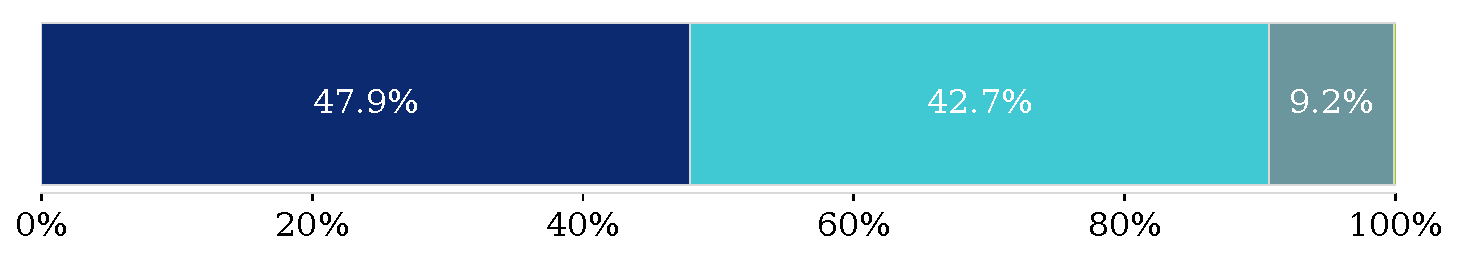
\includegraphics[width=\textwidth]{\ChartsDir/rq2-topup-methods}
	\caption{\rqshorttext{cashflow-top-up-balance} Top-Up Transactions by Payment Method}
	\label{chart:top-up-transactions-by-payment-method}
	\source
\end{chart}

Thanks to the results, it is clear how many funds the system received and by what means.

\begin{keytakeaways}
	\begin{itemize}
		\item The total top-up amount was~\bfmtczk{14520973}.
		\item The most used payment method was the card terminal at the event with~\bfmtnump[1]{47.9}\%~of all top-ups.
		\item Only a little over~\bfmtnum{9}\% of the top-ups were done online.
	\end{itemize}
\end{keytakeaways}

%%% Cashflow / Sales Analysis
%%% --------------------------------------------------------------

\subsection{Sales Analysis}
\label{subsec:analysis-sales}

\makerqbox{cashflow-total-sales}

The sales analysis was crucial for understanding the overall sales behavior and served as a basis for further insights tightly connected to the revenue sources.

To answer the research question, it was necessary to find all sales transactions and their respective sellers and to divide them into two groups: the direct organizer's sales and external vendors' sales.
And for better understanding, the sales were also grouped by the product categories (see~\autoref{tab:product-categories} for the list of categories).

The results show that the total sales of the event were~\bfmtczk{11711807} with the organizer's sales being~\bfmtczk{8240264} and the external vendors' sales being~\bfmtczk{3471543}.

The organizer, most importantly, sold all the beer beverages and most of the non-alcoholic and alcoholic (spirits) beverages.
Whereas the external vendors sold mainly the food, wine, and other uncategorized products.
This can be seen in~\autoref{chart:sales-organizer-vs-vendors} below.

\begin{chart}[h]
	\centering
	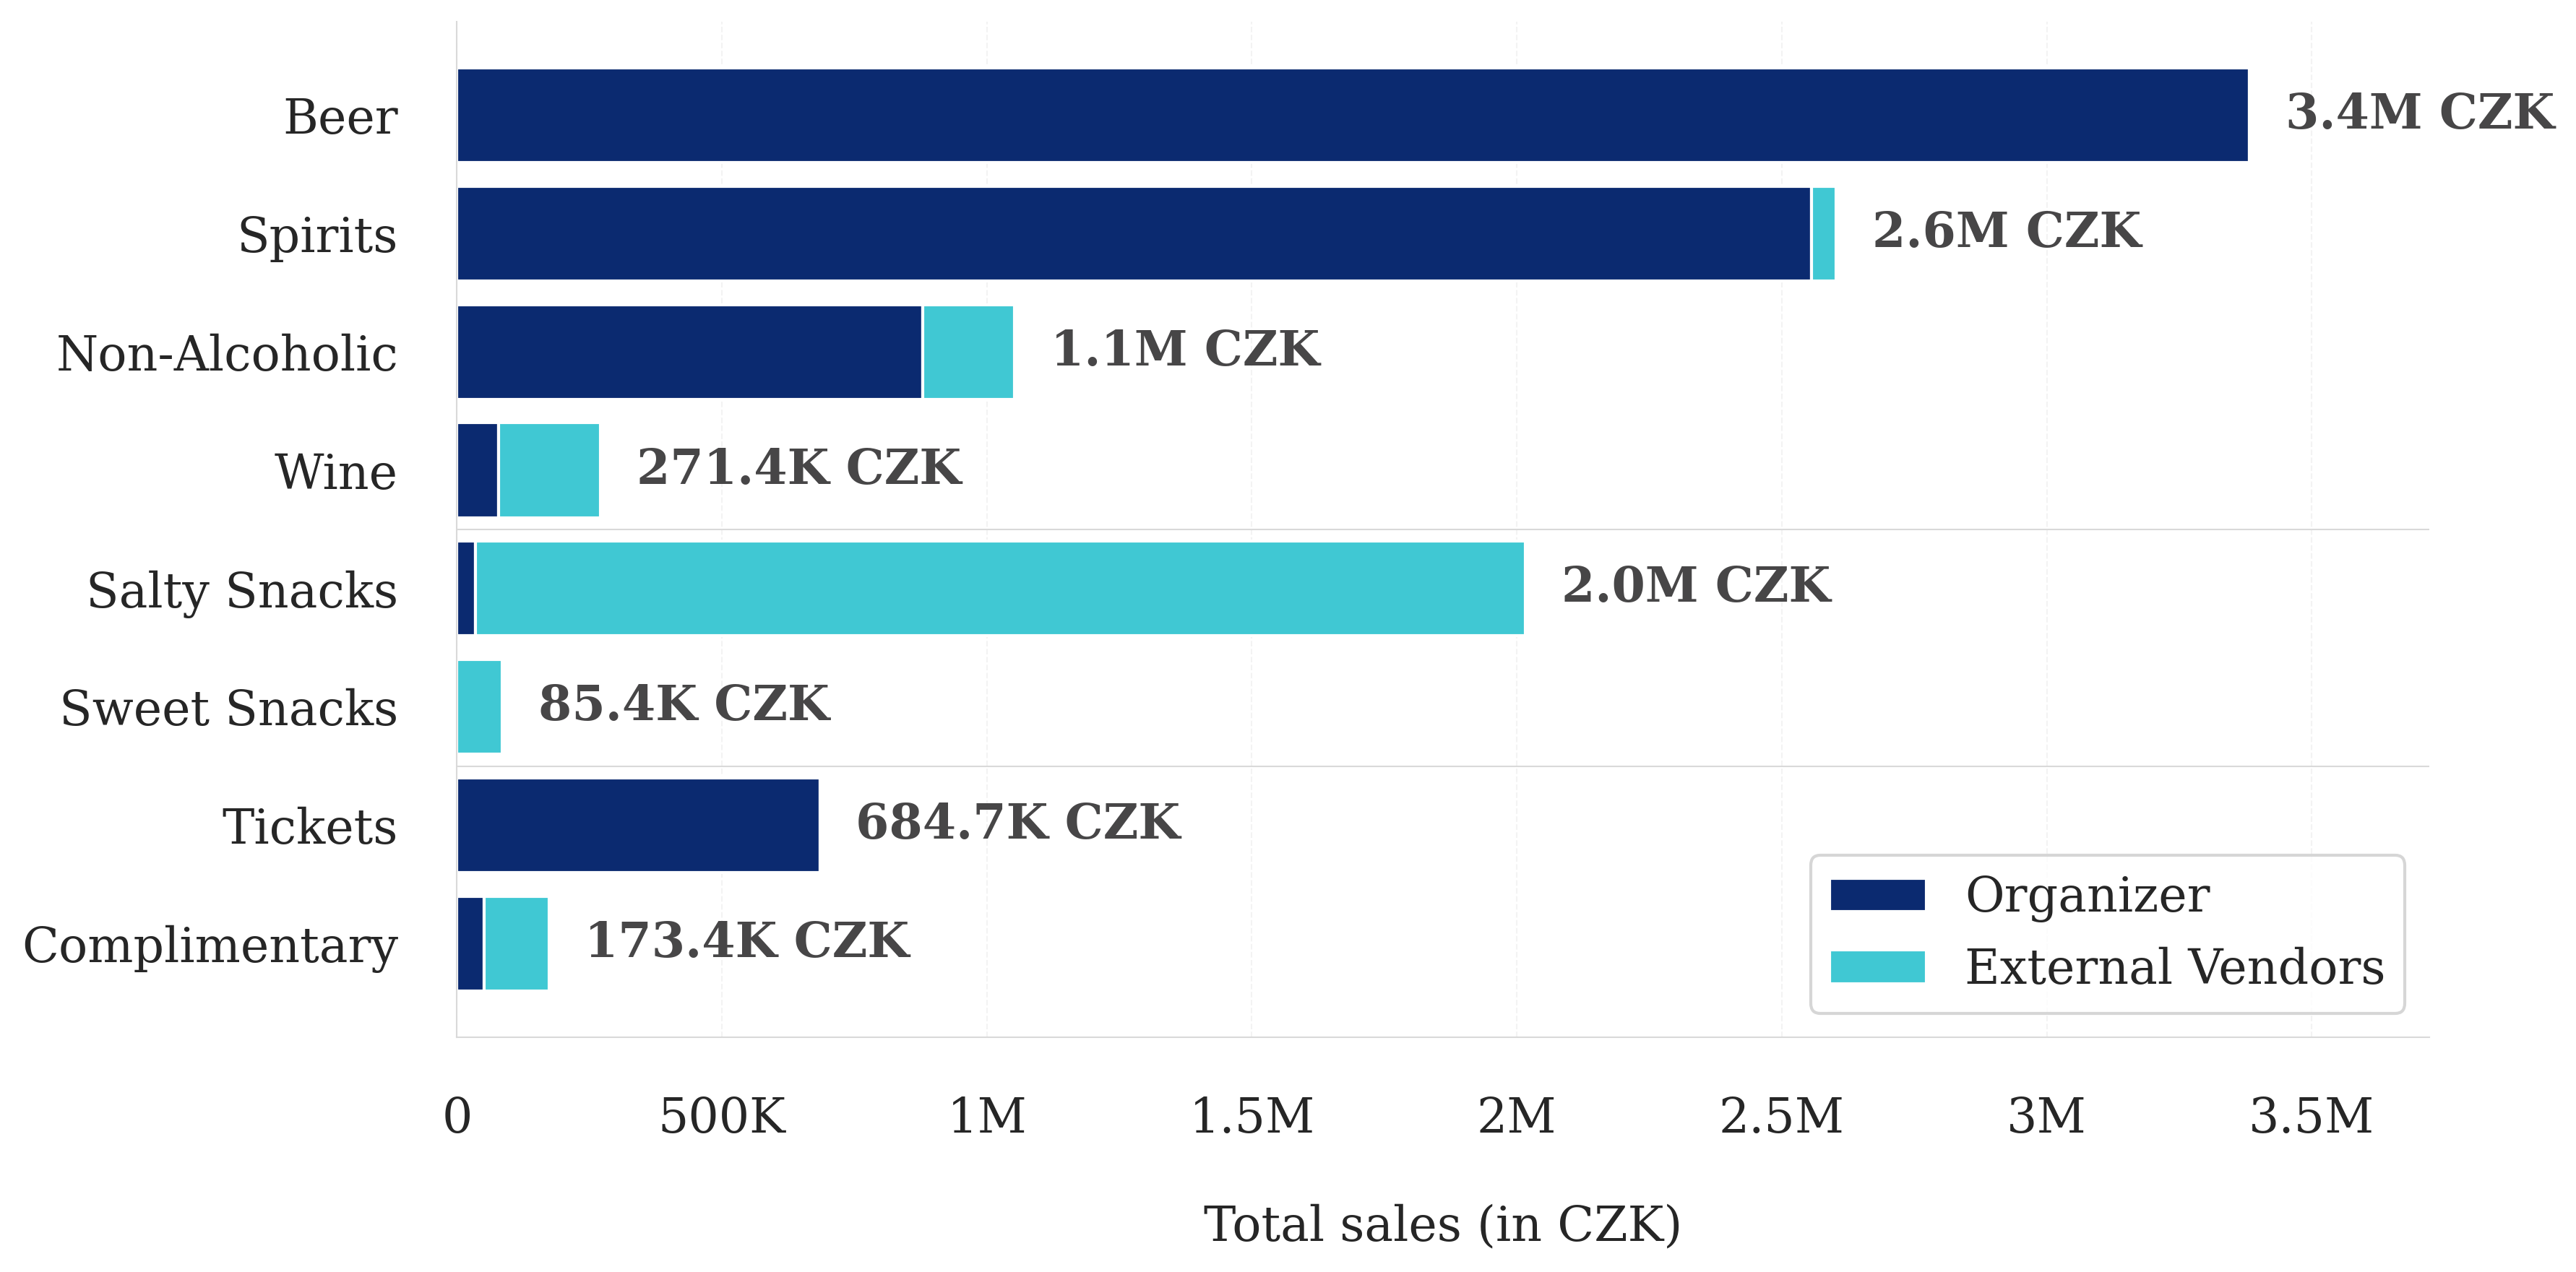
\includegraphics[width=\textwidth]{\ChartsDir/rq4-organizer-vs-vendor-sales}
	\caption{\rqshorttext{cashflow-total-sales} Sales of the Organizer vs. External Vendors}
	\label{chart:sales-organizer-vs-vendors}
	\source
\end{chart}

The organizer also sold not so few of the uncategorized products, which after further investigation turned out to be ticket sales at the event amounting to~\bfmtczk{684700}.

In total, the organizer direct sales were \textbf{70\%} of the total sales, which is a significant portion, and thus the organizer itself has even bigger influence on the event's financial performance.

\begin{keytakeaways}
	\begin{itemize}
		\item Total sales of the event were~\bfmtczk{11711807}, where organizer's sales were~\textbf{70\%} of the total.
		\item The organizer sold all beer beverages and the majority of the non-alcoholic and alcoholic beverages.
		\item The organizer also sold tickets at the event amounting to~\bfmtczk{684700}.
		\item External vendors sold food, wine, and other uncategorized products.
	\end{itemize}
\end{keytakeaways}


%%% Cashflow / Remaining Chip Balances
%%% --------------------------------------------------------------

\subsection{Remaining Chip Balances}
\label{subsec:analysis-remaining-balances}
\makerqbox{cashflow-remaining-balance}

The remaining chip balances are crucial for the event organizer as they represent the potential revenue that can still be claimed.
Any unclaimed balances following a specified refund period, typically up to 14~days post-event, will be deemed taxable revenue for the organizer.

Out of the total top-up amount of~\bfmtczk{14520973}, the total spent credit amounted to~\bfmtczk{10984945}, which left a total of~\bfmtczk{3536028} on the chips before refunds.
After refunds – done both at the event (\bfmtczk{15379}) and later via online bank refund requests (\bfmtczk{3163567}) – the remaining balance was reduced to~\bfmtczk{357082}.

However, this still included the artificially issued VIP credits with leftover balance of~\bfmtczk{12405}.
The system also reported integrity errors in the data, which resulted in a total of~\bfmtczk{10246}~due to fraudulent activities performed by some attendees which were automatically suspended by the system.

This left the total unclaimed balance at~\bfmtczk{334431}, which could have been claimed by the organizer as taxable revenue.

Since these numbers can be quite abstract, the results in a form of sankey diagram in~\autoref{chart:remaining-balances-sankey}~below provide a more accurate representation.

\begin{chart}[h]
	\centering
	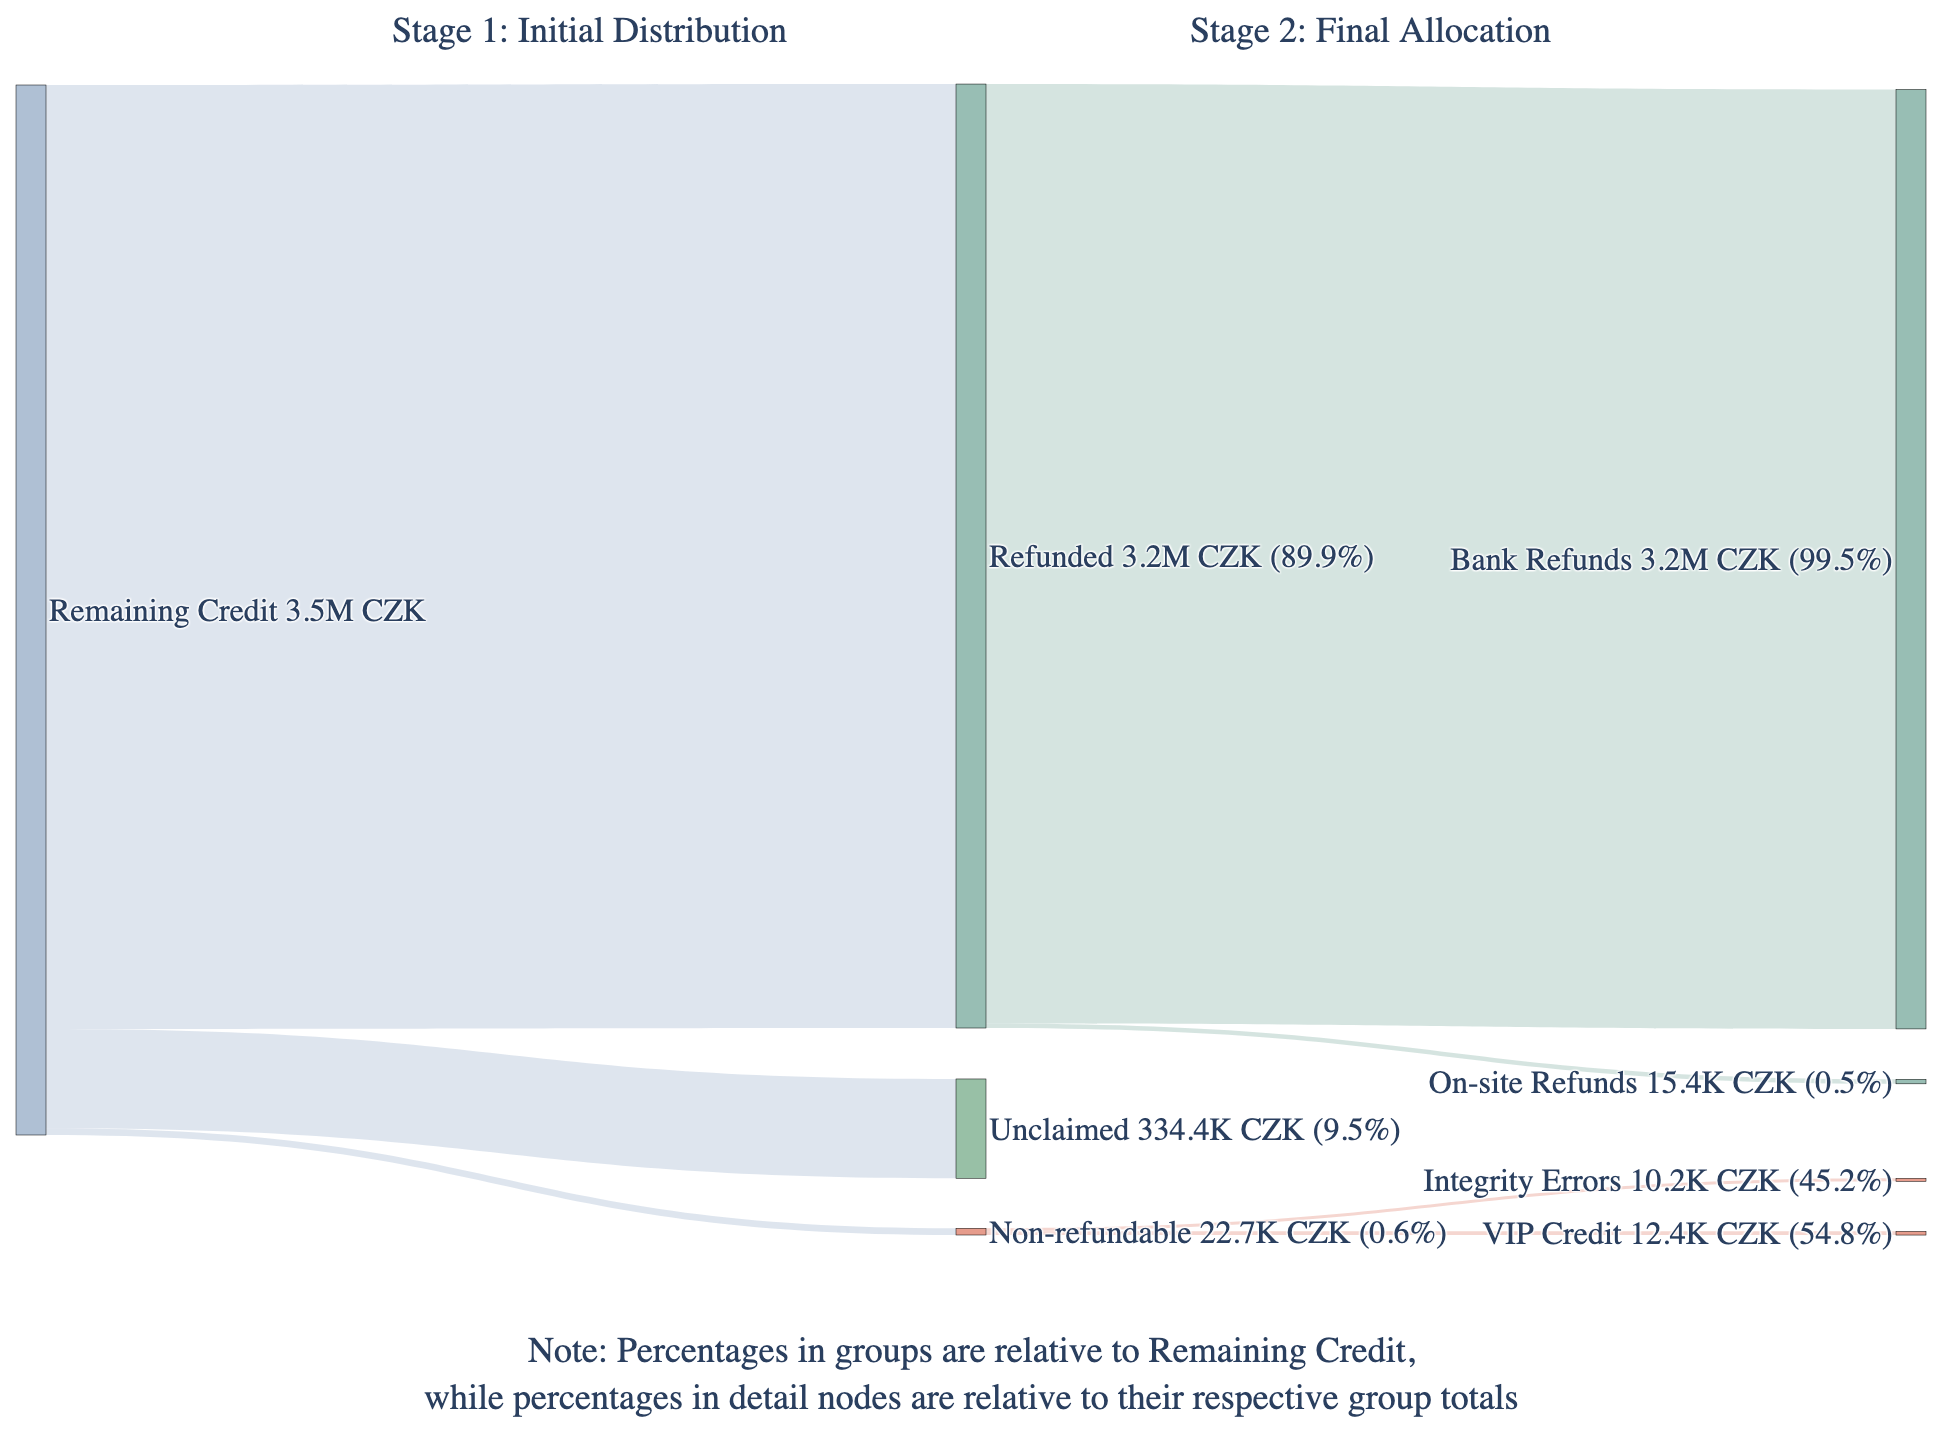
\includegraphics[width=\textwidth]{\ChartsDir/rq3-remaining-balances}
	\caption{\rqshorttext{cashflow-remaining-balance} Remaining Chip Balances Sankey Diagram}
	\label{chart:remaining-balances-sankey}
	\source
\end{chart}

Thanks to this breakdown, it is clear how the remaining balances were reduced and what was the outcome.
These results are important for the last part of this section, which is the total revenue of the organizer.

\begin{keytakeaways}
	\begin{itemize}
		\item Total unused credit was~\bfmtczk{3536028}.
		\item Credit refunded to customers was~\bfmtczk{3178946}.
		\item After VIP issued credits and system integrity error, the unclaimed balance was~\bfmtczk{334431}.
	\end{itemize}
\end{keytakeaways}

%%% Cashflow / Total Revenue of the Organizer
%%% --------------------------------------------------------------

\subsection{Total Revenue of the Organizer}
\label{subsec:analysis-total-revenue}
\makerqbox{cashflow-total-revenue}

The festival's financial model is based on a combination of revenue streams.

The most important stream is the \textbf{commission from the vendor sales}, which is arranged in advance between the organizer and the vendors.
The commission is, in this case, a percentage (ranging from 15\% to 30\% depending on the deal) of the vendor sales amount without VAT\@.

Therefore, this required finding all sales transactions made at the external vendors' stands and calculating the commission based on the agreed percentage.
However, this was not a straightforward task, since a transaction could contain multiple products even from different vendors.

This required a more complex calculation, for which were used the previously mentioned data processing views which were designed for this purpose.
In the end, the total revenue from sales commissions was~\bfmtczkp[2]{820712,79}.

Another source of revenue is the \textbf{unclaimed chip balances}, which, after a credit refund period, are considered as taxable revenue for the organizer.
This, thanks to the previous subsection, was found to be~\bfmtczk{334431}.

Currently totalling~\bfmtczkp[2]{1155143,79} is the direct revenue of the organizer from the event.
However, given the circumstances and setup of this event, there were also additional, but indirect revenue streams that were not included in the total revenue.
These include \textbf{the online ticket sales}, which were sold by the organizer and \textbf{the direct sales of the organizer}.
They were not included in the total direct revenue, as they may misinterpret the results since the analysis lacks expenses of the organizer.

If we were to include these, the total revenue would increase by~\bfmtczk{11179700} from the online ticket sales and by~\bfmtczk{8240264} from the direct sales, which would result in a total revenue of~\bfmtczkp[2]{20575107,79}.

To better understand the revenue streams, the results are visualized in~\autoref{chart:revenue-breakdown-total}~below.

\begin{chart}[h]
	\centering
	% chart
	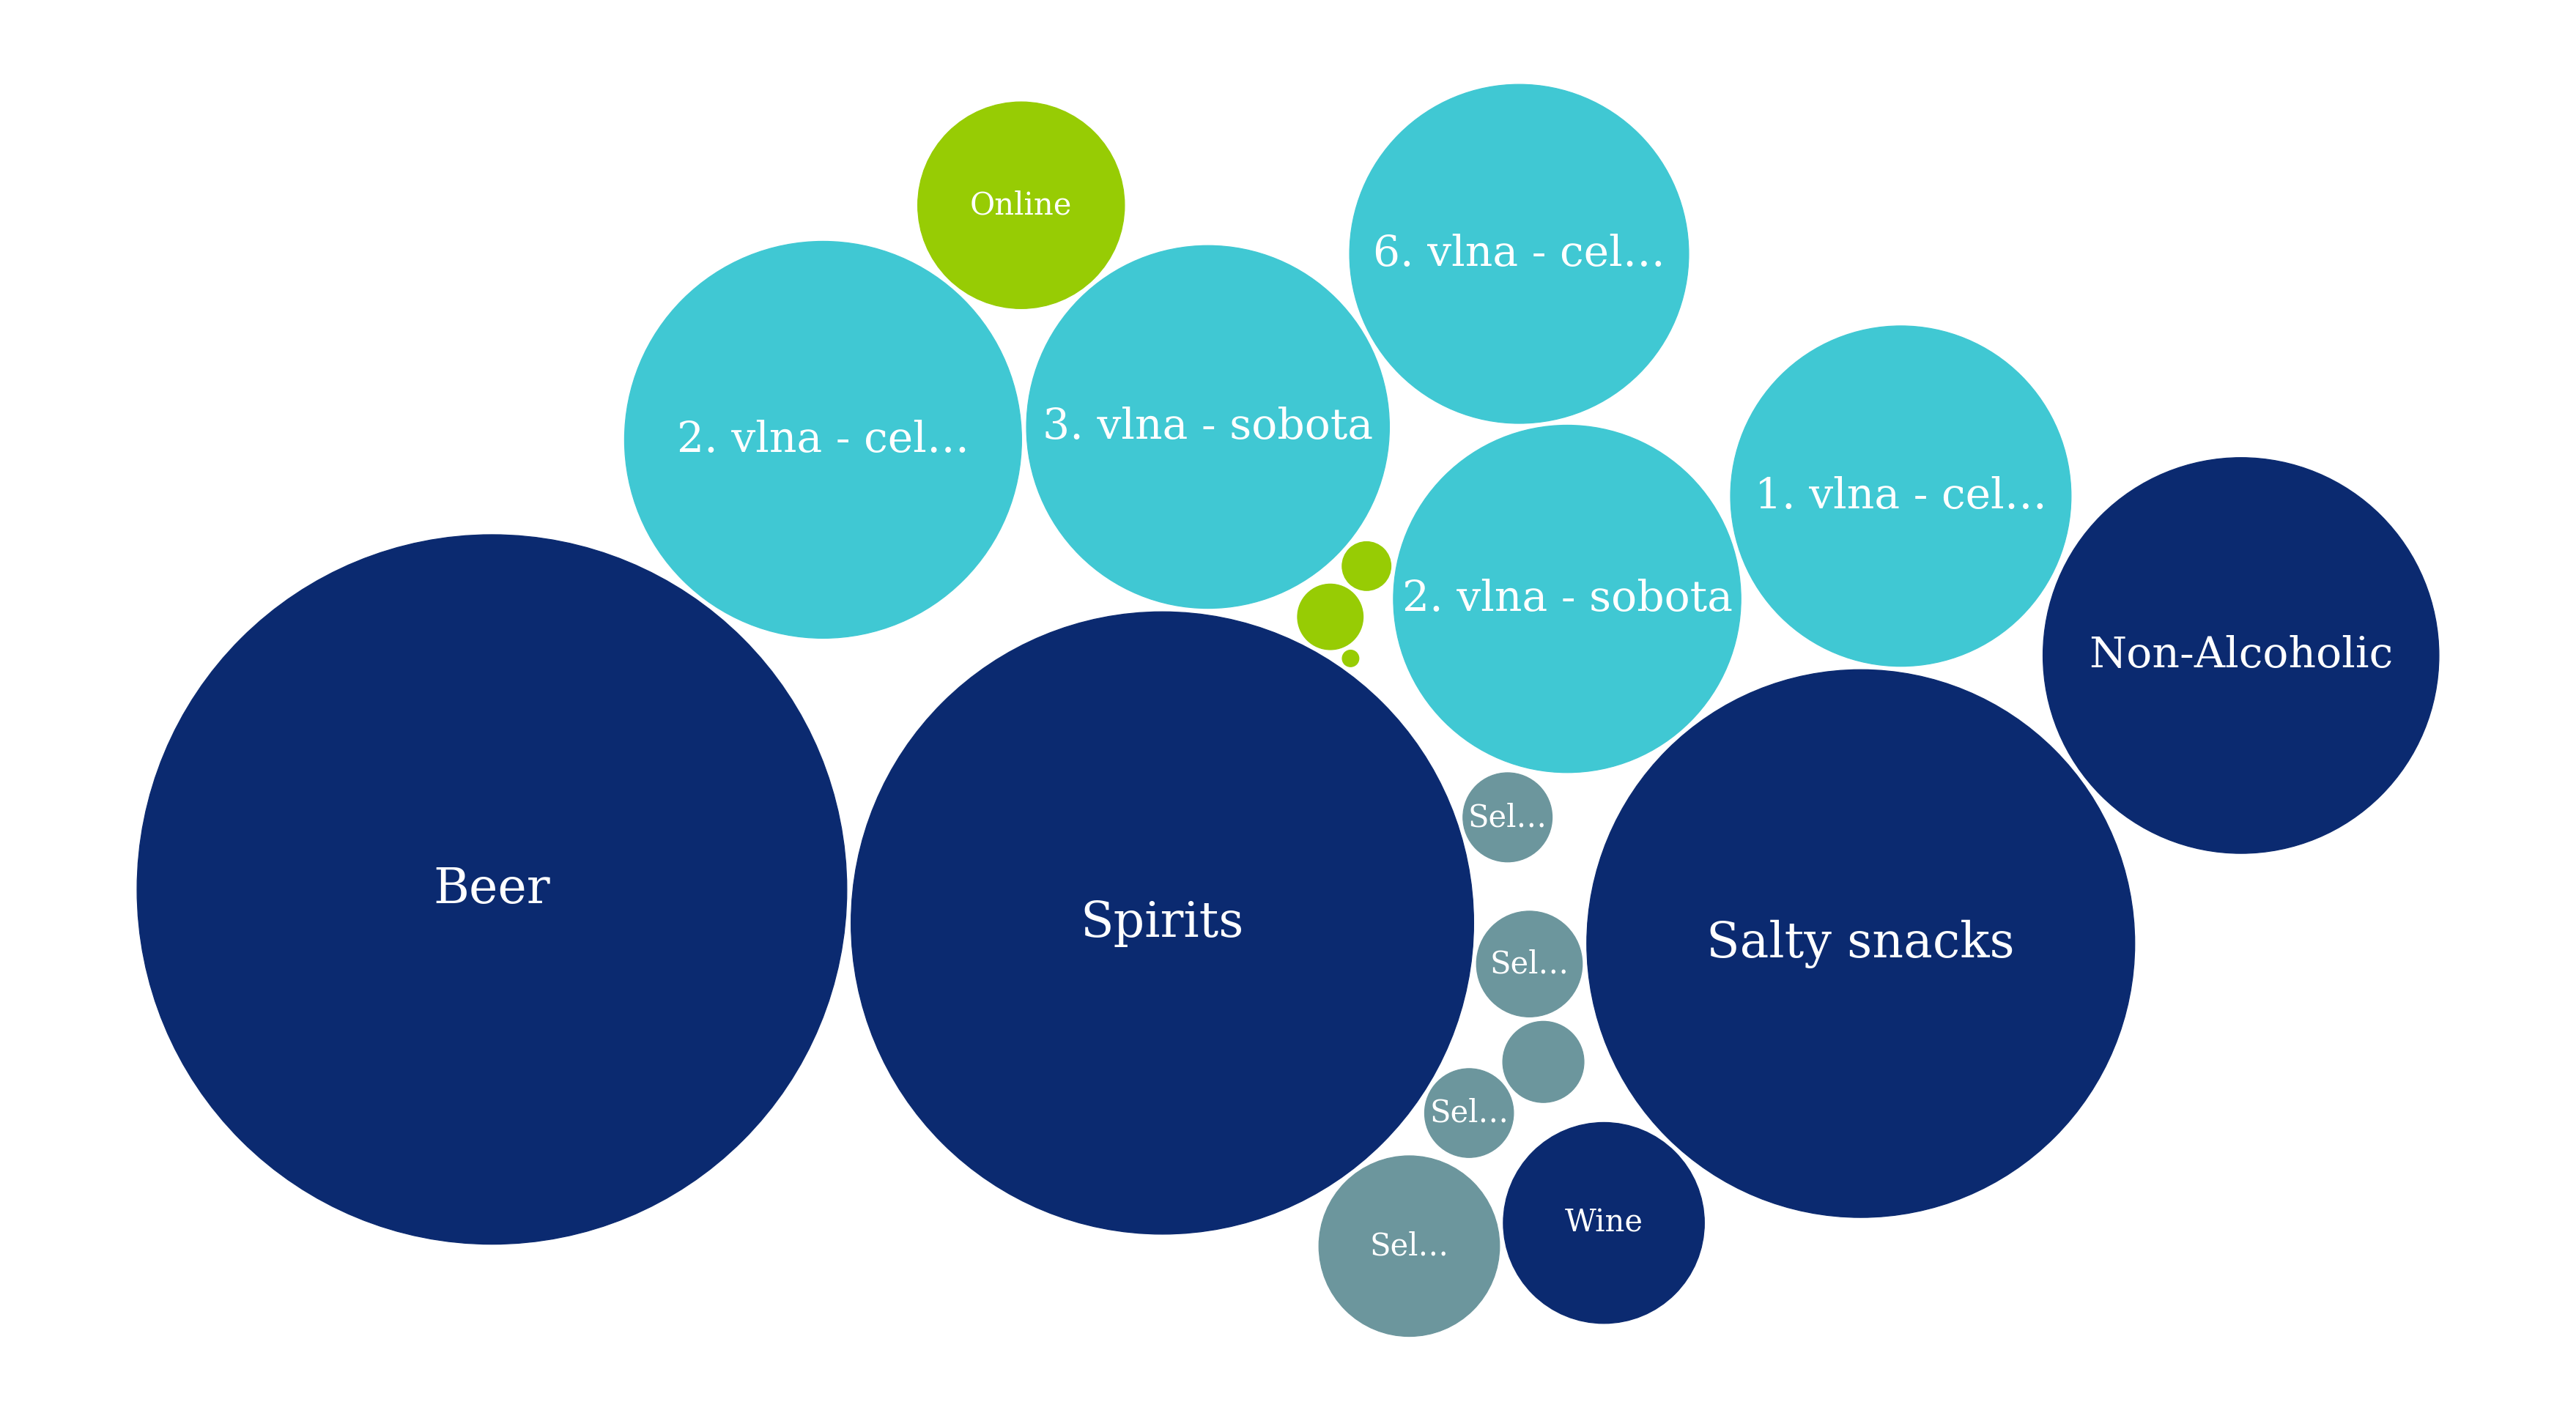
\includegraphics[width=\textwidth]{\ChartsDir/rq1-total-revenue-breakdown}
	% space
	\par\vspace*{0.5em}
	% table
	% @formatter:off
	\begin{tabularx}{\textwidth}{|>{\columncolor{unicorn_blue!5}}X|>{\columncolor{unicorn_blue!5}}r|}
		\hline
		\rowcolor{unicorn_blue}
		\textbf{\color{white}Revenue Stream} & \textbf{\color{white}Amount} \\
		\hline
		\hline
		\colorindicator{3}Vendor Commissions & \fmtczkp[2]{820712.79} \\
		\colorindicator{4}Unclaimed Chip Balances & \fmtczk{334431} \\
		\hline
		\textbf{Total Direct Revenue} & \bfmtczkp[2]{1155143.79} \\
		\hline
		\colorindicator{2}Online Ticket Sales & \fmtczk{11179700} \\
		\colorindicator{1}Organizer Direct Sales & \fmtczk{8240264} \\
		\hline
		\textbf{Total Revenue (All Streams)} & \bfmtczkp[2]{20575107.79} \\
		\hline
	\end{tabularx}
	% @formatter:on
	\caption{\rqshorttext{cashflow-total-revenue} Breakdown of All Revenue Streams}
	\label{chart:revenue-breakdown-total}
	\source
\end{chart}

\begin{keytakeaways}
	\begin{itemize}
		\item Total direct revenue of the organizer was~\bfmtczkp[2]{1155143,79}.
		\item Vendor sale commission contributed to~approximately 71\% of the total direct revenue.
		\item With other indirect revenue streams, the total revenue would be~\bfmtczkp[2]{20575107,79}.
	\end{itemize}
\end{keytakeaways}

\pagebreak[4]

%%% Cashflow / Summary
%%% --------------------------------------------------------------

\subsection{Summary}
\label{subsec:analysis-cashflow-summary}

This section provided a comprehensive view of the festival's financial performance and cash flows.
The results covered the top-up transactions, sales analysis, remaining chip balances, and the total revenue of the organizer and contributed to a better understanding from the financial perspective of the festival.

Nevertheless, results covered in these subsections are only a part of the whole picture and can be interpreted in various ways.

For this particular challenge, a summarized cash flow diagram of event payments was created, however, with online ticket sales excluded from the total indirect revenue.
This diagram can be seen in~\autoref{chart:cash-flow-diagram} below.

\begin{chart}[h]
	\centering
	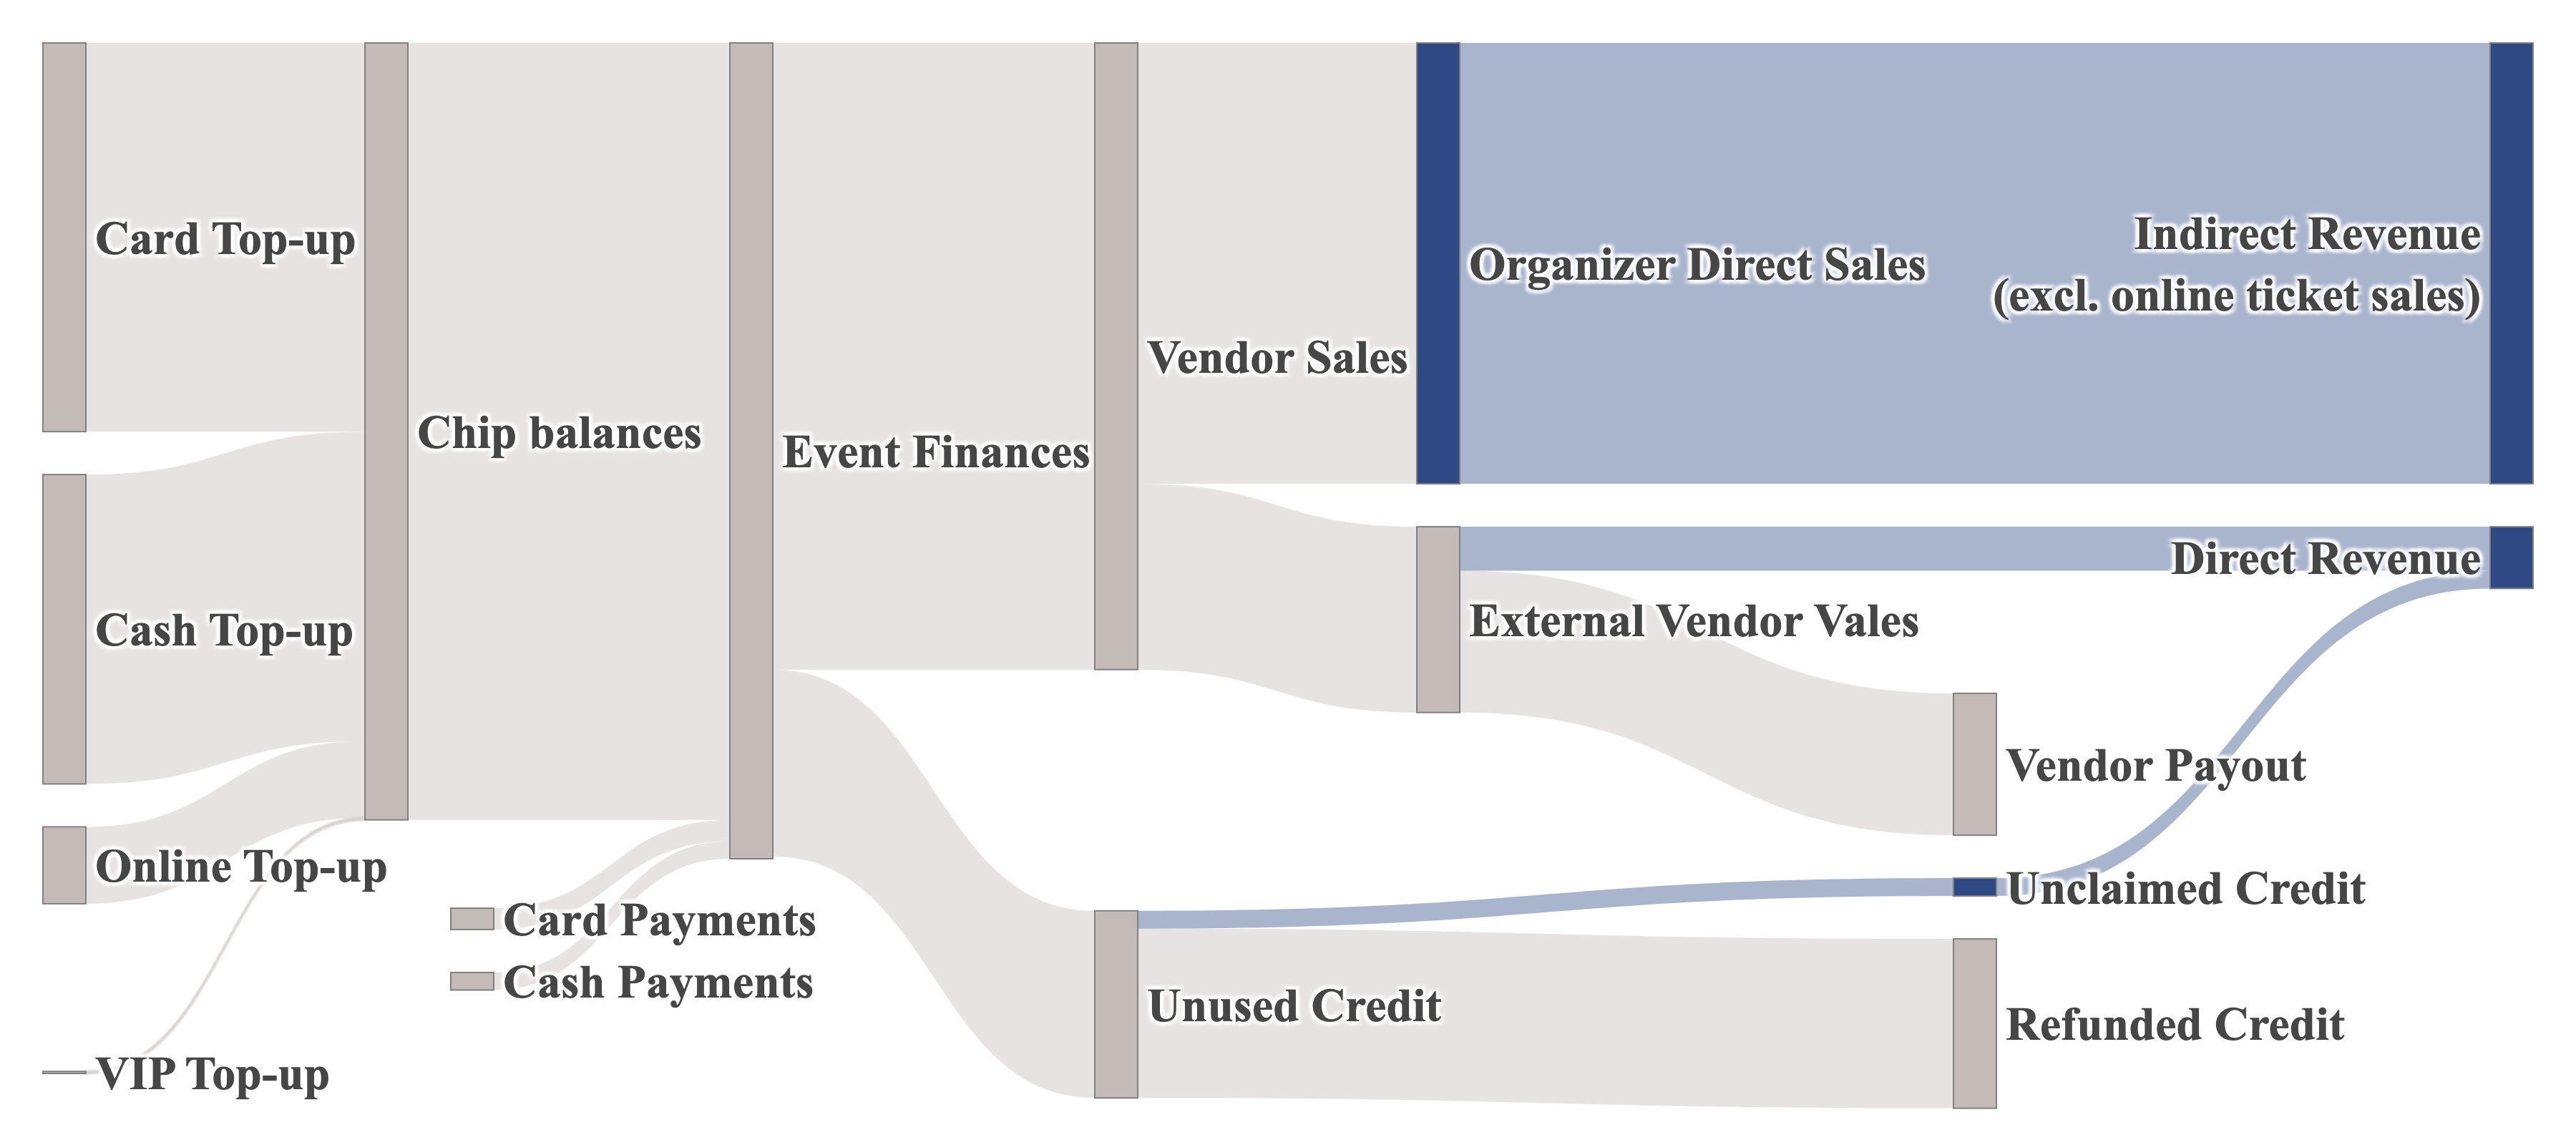
\includegraphics[width=\textwidth]{\ChartsDir/total-revenue-cashflows}
	\caption{Overall Cash Flow Diagram}
	\label{chart:cash-flow-diagram}
	\source
\end{chart}

This diagram provides a clear overview of the financial flows during the festival and nicely summarizes the results of this analysis.

\begin{keytakeaways}
	\begin{itemize}
		\item The total incoming money flow was~\bfmtczk{14520973} from top-ups and~\bfmtczk{726862} from non-chip sales.
		\item Total sales amounted to~\bfmtczk{11711807}.
		\item After refunds, the remaining balance left was~\bfmtczk{334431}.
		\item Commission from external vendor sales was~\bfmtczkp[2]{820712,79}.
		\item The total direct revenue of the organizer was~\bfmtczkp[2]{1155143,79}.
	\end{itemize}
\end{keytakeaways}

%%% Section: Performance Indicators Analysis
%%% --------------------------------------------------------------


\section{Performance Indicators Analysis}
\label{sec:analysis-performance-indicators}

This section emphasizes the event's performance metrics.
The goal is to identify key metrics that can be used to further evaluate the event and its success.
The potential of this analysis is to measure the~\enquote{greatness}~and the size of the event in terms of performance.

This analysis aims to provide answers to previously defined research questions about the event's performance.
For this analysis, they were slightly reordered and grouped into the two subsections listed below:
\begin{enumerate}
	\item \fullref{subsec:analysis-performance-indicators-transactions}
	\item and~\fullref{subsec:analysis-performance-indicators-best}
\end{enumerate}

The results of this analysis should provide insights into the event's performance and help the organizer to understand the key metrics that can be used to evaluate the event's success.

%%% Performance / Transactions Processing Analysis
%%% --------------------------------------------------------------

\subsection{Transactions Processing Analysis}
\label{subsec:analysis-performance-indicators-transactions}

This subsection will focus on the processing of transactions during the event in pursuit of answering the three first research questions of this section.

\makerqbox{performance-transactions}

This question actually consists of two sub-questions, which will be addressed separately.

The first part questions the total number of transactions processed during the event.
This was actually quite simple to answer, as the system was designed to track all transactions and their types.
The resulting total number of transactions was~\bfmtnum{141381} consisting of~\bfmtnum{110854}~sales transactions, \bfmtnum{17726}~top-up transactions and~\bfmtnum{12801}~chip register transactions.

The second part focuses on rather time-related metrics and asks about the processing peak times during the festival.
For this part, it was necessary to spread out the above transactions over time and find the peaks.

The results in~\autoref{chart:transactions-peaks} below show the distribution of the processed transactions over time.
It clearly identifies the peak on the last day of the festival at 18:00, amounting to~\bfmtnum{8986}~transactions.

\begin{chart}[H]
	\centering
	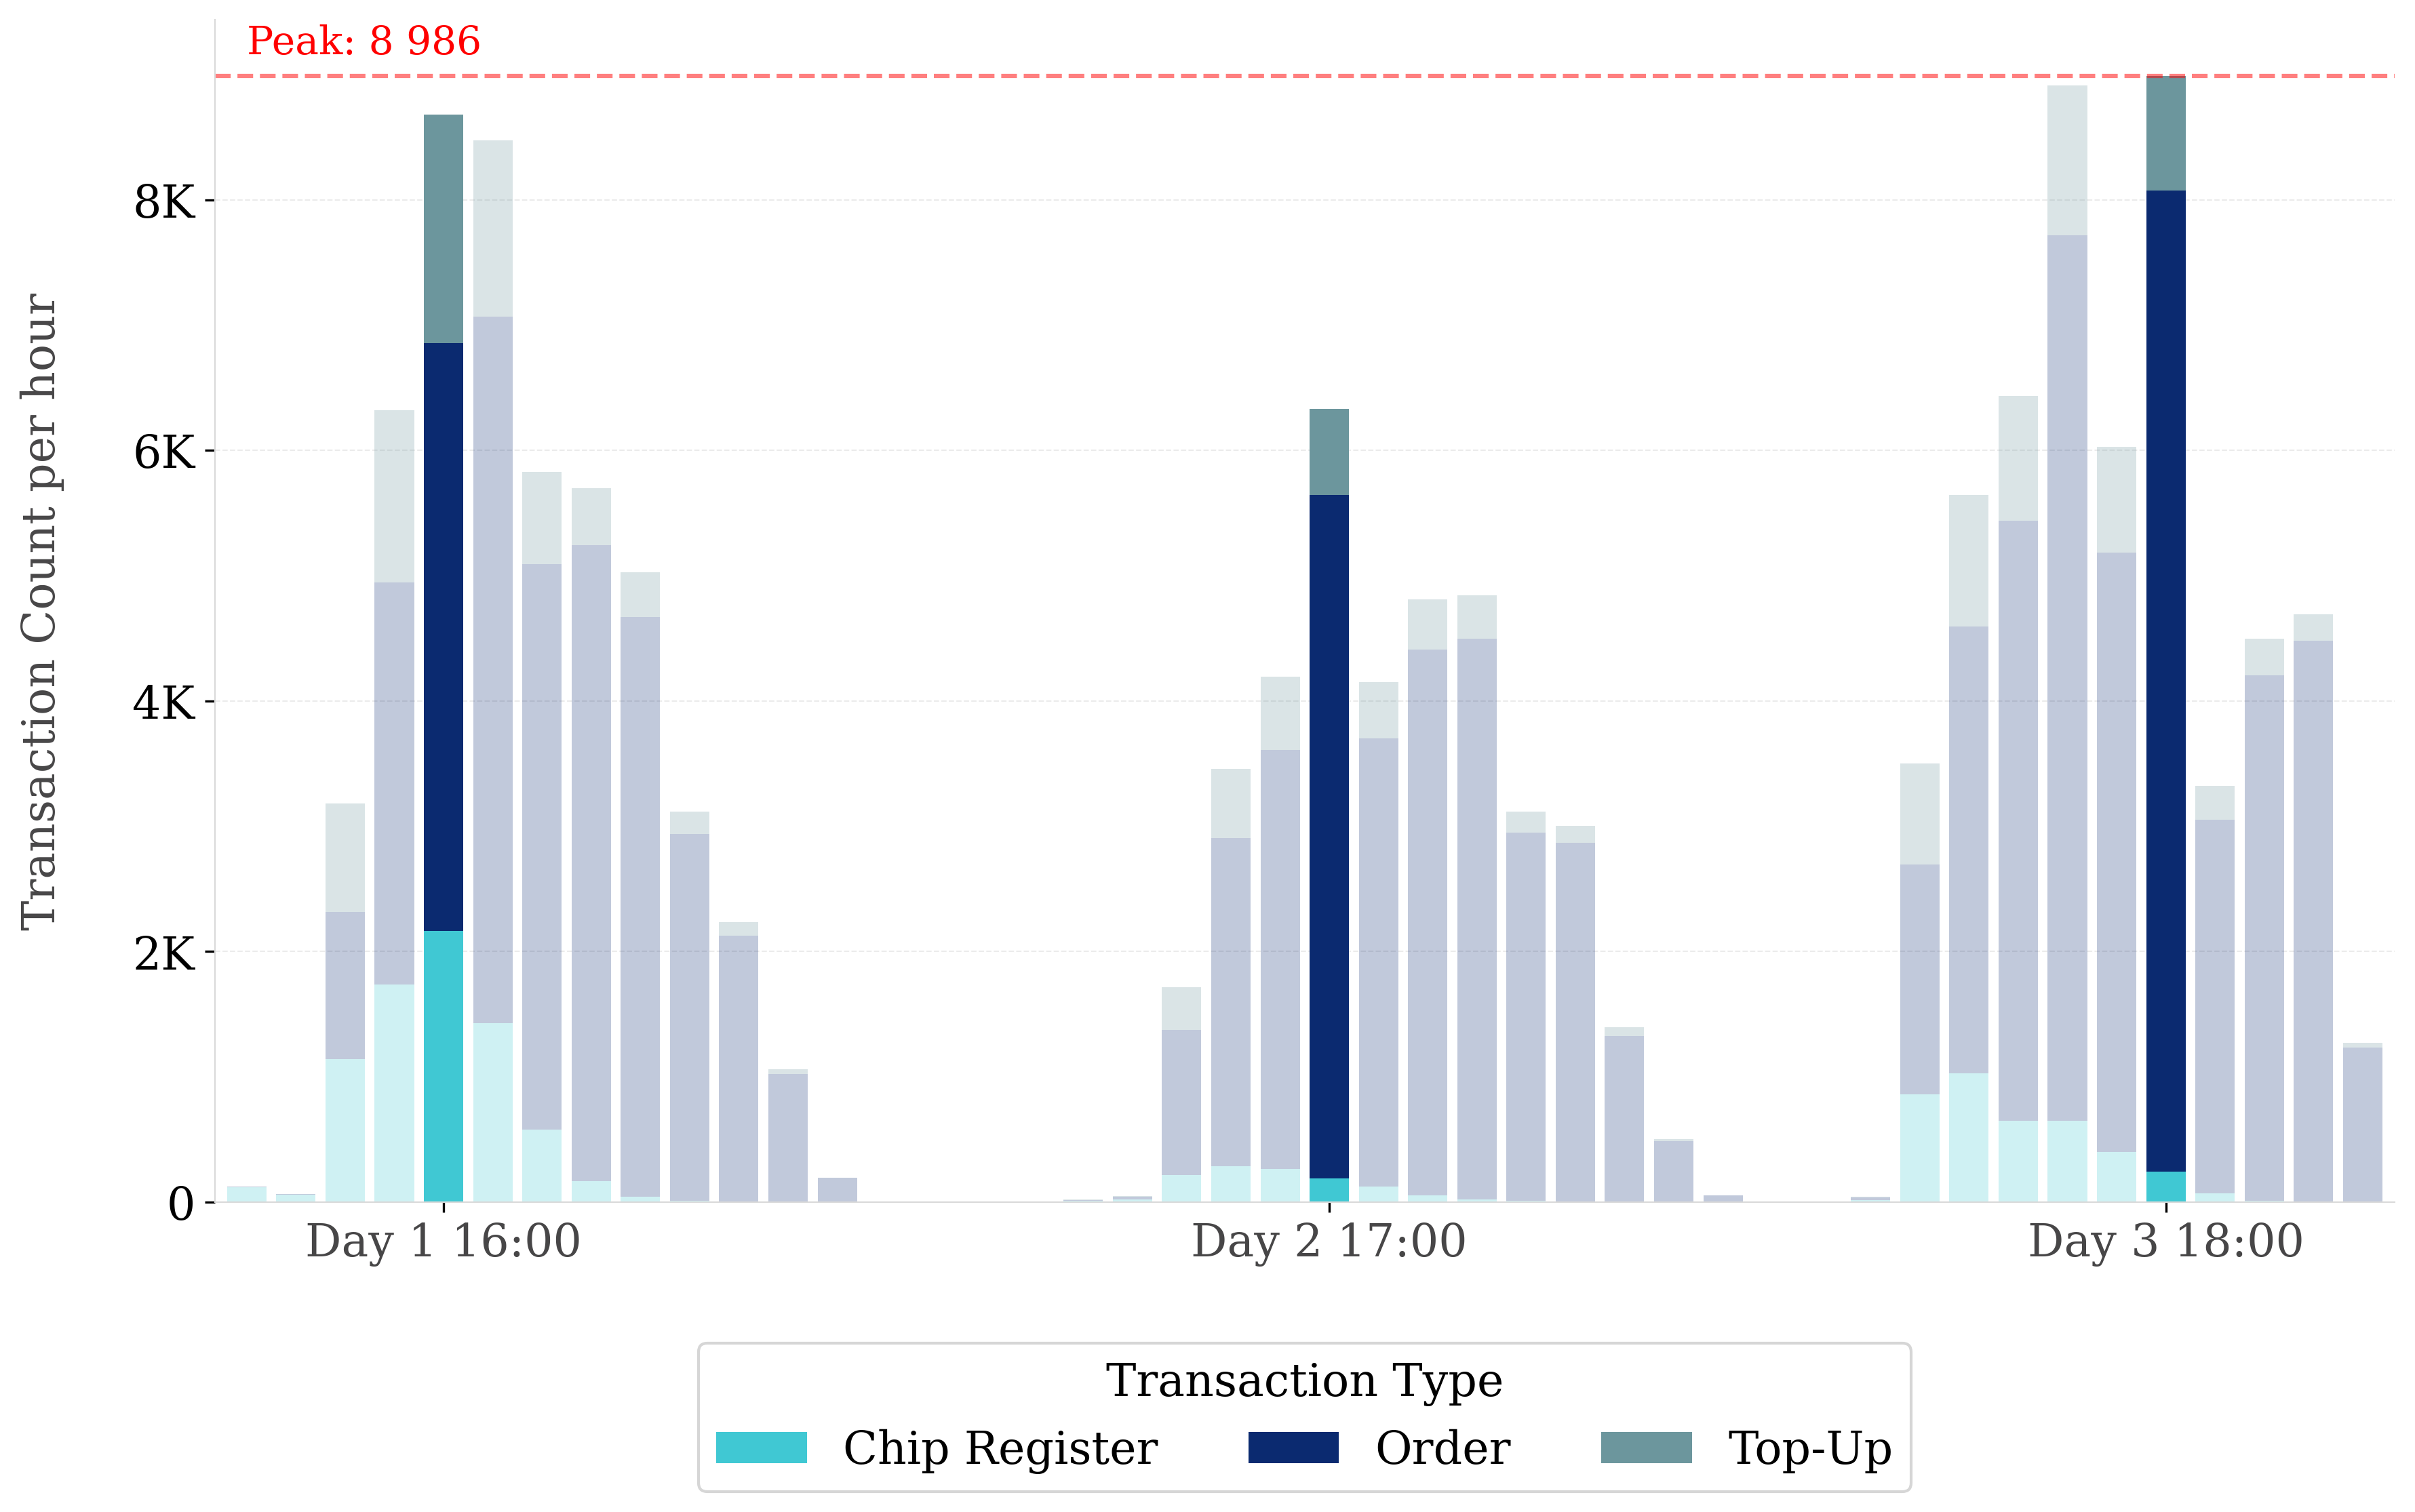
\includegraphics[width=\textwidth]{\ChartsDir/rq5-transaction-peaks}
	\caption{\rqshorttext{performance-transactions} Transactions Peaks}
	\label{chart:transactions-peaks}
	\source
\end{chart}

\begin{keytakeaways}
	\begin{itemize}
		\item Total number of transactions processed was~\bfmtnum{141381} consisting mainly (\bfmtnum{78}\%) of order transactions.
		\item The peak in processed transactions was on the last day of the festival at 18:00 with~\bfmtnum{8986}~transactions processed at that hour.
	\end{itemize}
\end{keytakeaways}

The following two questions (\rqshort{performance-processing-during-peaks}~and~\rqshort{performance-delays-downtimes}) focus on processing times and potential delays during the event.

\makerqbox{performance-processing-during-peaks}

The answer to this question is closely related to the previous one, as it requires the identification of the processing times during the peak times, which were already previously identified.

\pagebreak[4]

It required finding the average processing time, meaning the difference between the transaction creation and its completion times.

\begin{infobox}{What causes the processing time?}
	The time when the transaction is created is the time when the in-place offline-supported system created the transaction, and the processed time is later when the central system receives the transaction and processes it.

	The delays can be caused by various factors, such as network latency, offline mode active, system load, or even the transaction type.
\end{infobox}

The results show that the average processing time during the peak times was approximately~\bfmtnum{25}~seconds.

When slightly changing the displayed data, we also get the answer to the~\rqshort{performance-delays-downtimes} about the potential delays and downtimes during the event.

\makerqbox{performance-delays-downtimes}

Results in~\autoref{chart:rq7-processing-times}~shows the distribution of the processing times over the time and identifies one high processing peak of approximately~\bfmtnum{11}~minutes.
This is highly unusual and indicates a vendor's misuse of their device or an enabled offline mode.

\begin{chart}[h]
	\centering
	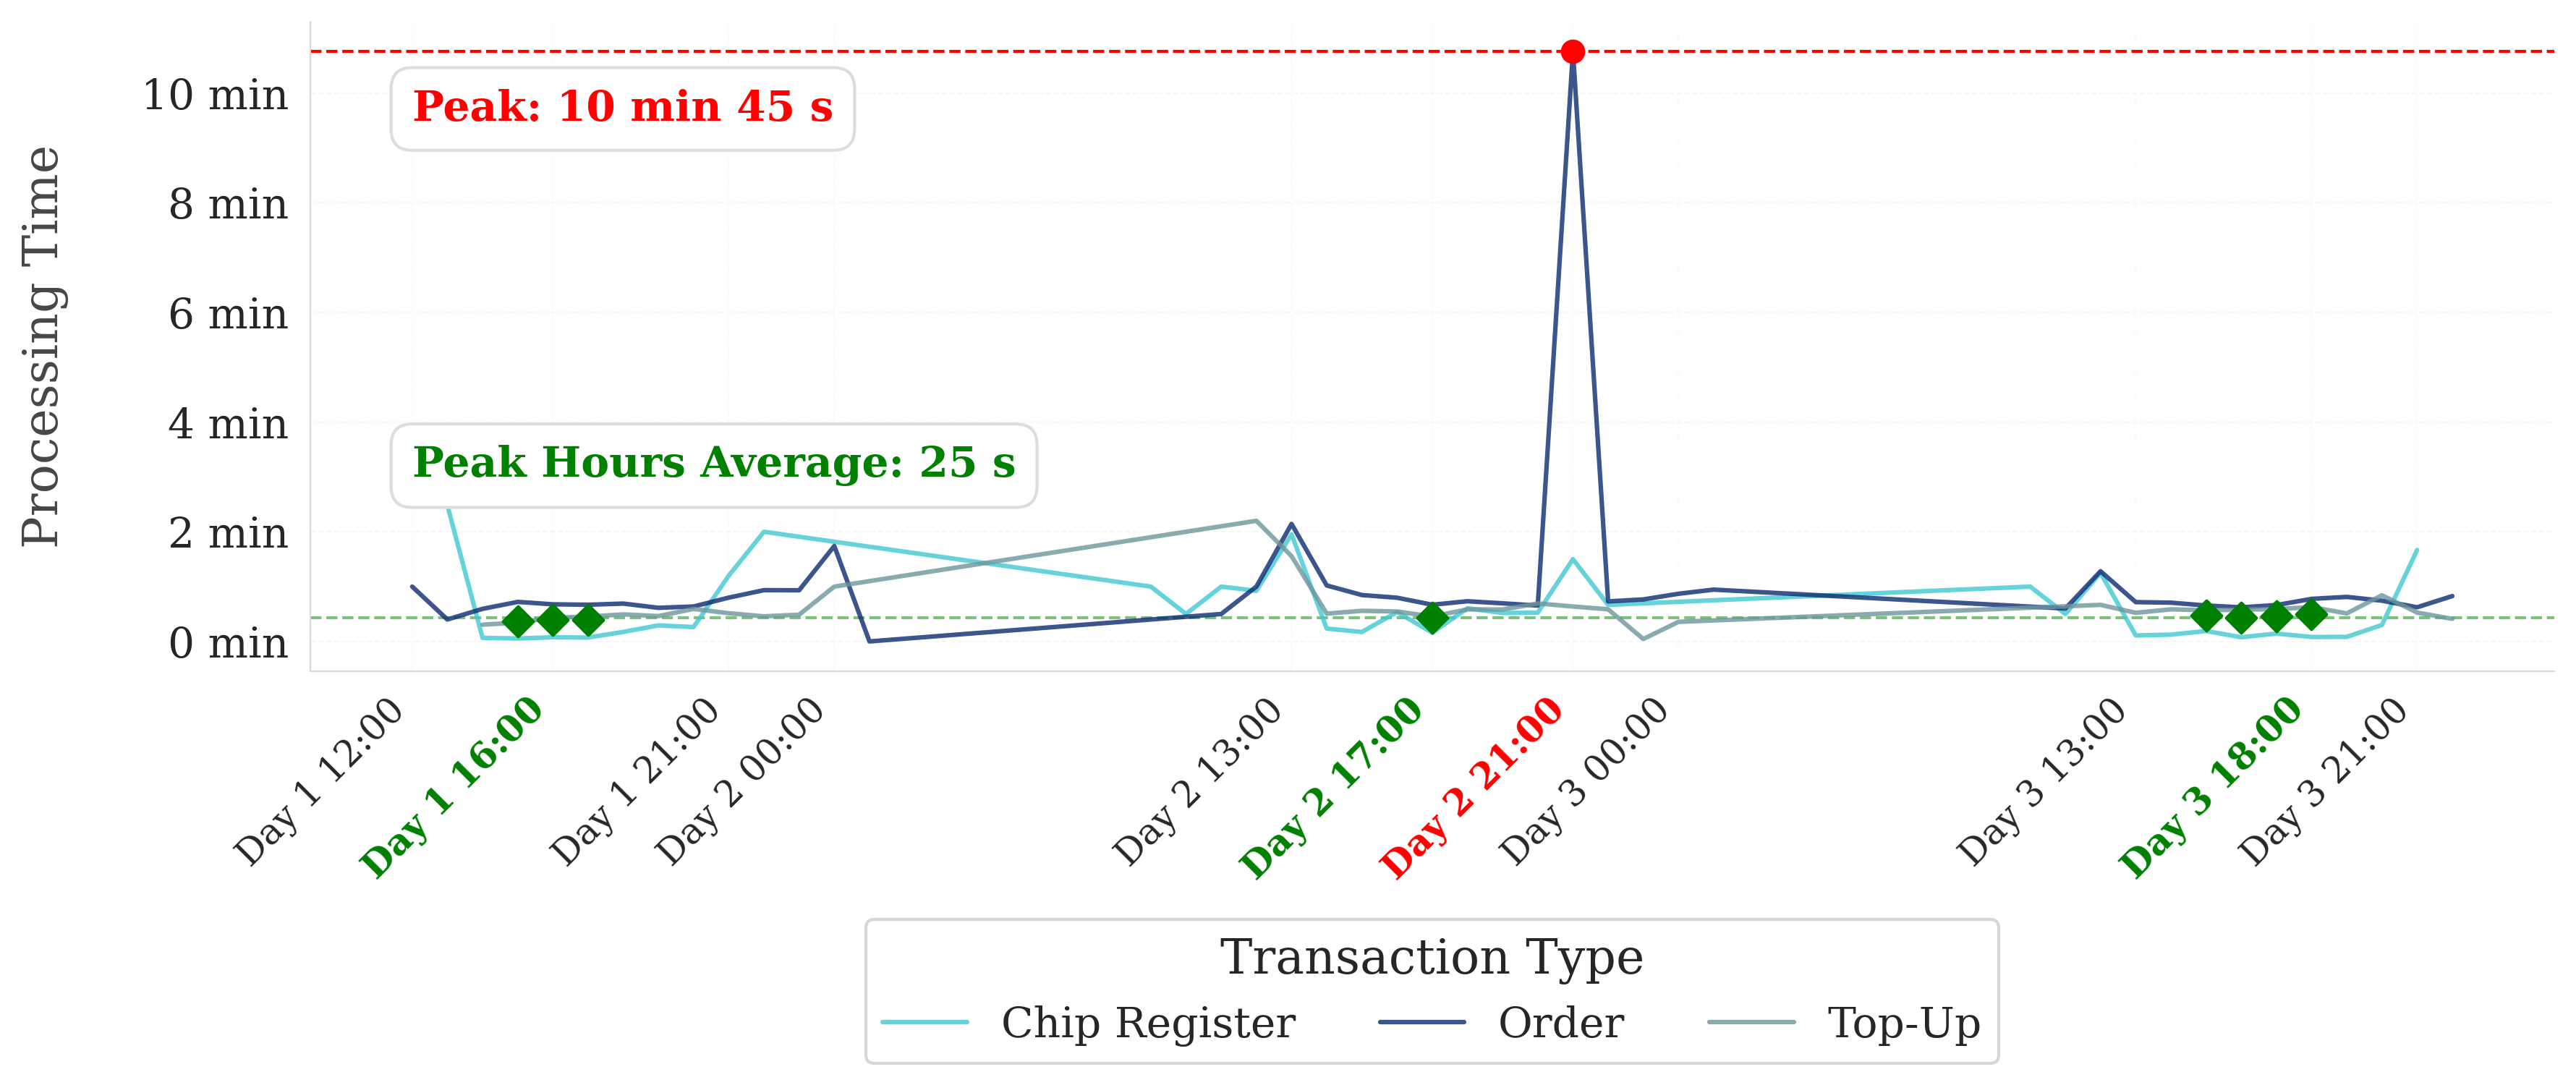
\includegraphics[width=\textwidth]{\ChartsDir/rq7-processing-times}
	\caption{\rqshorttext{performance-delays-downtimes} Transaction Processing Times}
	\label{chart:rq7-processing-times}
	\source
\end{chart}

Other high peaks are visible on the second day in the afternoon with approximately~\bfmtnum{2}~minutes processing time, which was probably caused by the initial load on that day.

\begin{keytakeaways}
	\begin{itemize}
		\item The average processing time during the peak times was~\bfmtnum{25}~seconds.
		\item The highest processing peak was approximately~\bfmtnum{11}~minutes, indicating a potential misuse of the system.
		\item Other high peaks were visible on the second day in the afternoon with approx.~\bfmtnum{2}~minutes processing time.
	\end{itemize}
\end{keytakeaways}

These results provide insights into the system's performance during the event, its reliability, and potential bottlenecks.
It also shows the festival's popularity and the system's ability to handle the load.

%%% Performance / Best Sale Places, Top-Up Points, Vendors, and Products Analysis
%%% --------------------------------------------------------------

\subsection{Best Sale Places, Top-Up Points, Vendors, and Products Analysis}
\label{subsec:analysis-performance-indicators-best}
In this subsection, the main goal will be to address the last four research questions of this section and provide insights into the best: sale places, top-up points, vendors, and products.

The problem with these question statements is that they are quite broad and can be interpreted in various ways.
What does a~\enquote{best} mean in this context?

It can be the most profitable, the best rated, the most visited, etc.
But since we are exploring the performance indicators, the best should be understood as the~\enquote{busiest}.
In terms of the system and this analysis, it should mean \textbf{the most transactions created} and possibly the point's ability to handle the load.

%%% Performance / Best Sale Places, Top-Up Points, Vendors, and Products Analysis / Best Sale Places
%%% --------------------------------------------------------------

\subsubsection{Best Top-Up Points}
\label{subsubsec:analysis-best-top-up-points}

The first focus will be on the best top-up points since unlike the sale places, vendors, and products, the top-up points are not linked to any specific product or vendor.

\makerqbox{performance-best-top-up-points}

To find these results, it required finding all top-up transactions, aggregating them in a bucket-like time frame and finally calculating their total counts, max peaks, and averages over time.

This resulted in the following findings in \autoref{tab:best-topup-points} below.

\begin{table}[htbp]
	\centering
	\small
	% @formatter:off
	\begin{tabularx}{\textwidth}{
		|>{\columncolor{unicorn_blue!5}\centering\arraybackslash}p{1cm}
		|>{\columncolor{unicorn_blue!5}\raggedright\arraybackslash}X
		|>{\columncolor{unicorn_blue!5}\raggedleft\arraybackslash}p{2.5cm}
		|>{\columncolor{unicorn_blue!5}\raggedleft\arraybackslash}p{2.5cm}
		|>{\columncolor{unicorn_blue!5}\raggedleft\arraybackslash}p{2.5cm}|}
		\hline
		\rowcolor{unicorn_blue}
		\textbf{}
		& \textbf{\color{white}Top-Up point}
		& \textbf{\color{white}Customers}
		& \textbf{\color{white}Transactions}
		& \textbf{\color{white}Max trx./h}
		\\\hline\hline
		% first rows
		\csvreader[
		head to column names,
		late after line={\\\hline},
		filter={\thecsvinputline<6}
		]{\DataDir/rq9-best-topup-points.csv}{
			entity=\colentity,
			customer_count=\colcustomers,
			transaction_count=\coltrxcount,
			max_hourly_peak=\colhourlypeak
		}{
			\the\numexpr\thecsvinputline-1
			& \colentity
			& \num[group-separator={,}]{\colcustomers}
			& \num[group-separator={,}]{\coltrxcount}
			& \num[group-separator={,}]{\colhourlypeak}
		}
		% separator
		\noalign{\vspace{1mm}}
		\multicolumn{5}{c}{\footnotesize{\textellipsis}}
		\\
		\noalign{\vspace{1mm}}
		\hline
		% middle rows
		\csvreader[
		head to column names,
		late after line={\\\hline},
		filter={\thecsvinputline>15 \AND \thecsvinputline<20}
		]{\DataDir/rq9-best-topup-points.csv}{
			entity=\colentity,
			customer_count=\colcustomers,
			transaction_count=\coltrxcount,
			max_hourly_peak=\colhourlypeak
		}{
			\the\numexpr\thecsvinputline-1
			& \colentity
			& \num[group-separator={,}]{\colcustomers}
			& \num[group-separator={,}]{\coltrxcount}
			& \num[group-separator={,}]{\colhourlypeak}
		}
		% separator
		\noalign{\vspace{1mm}}
		\multicolumn{5}{c}{\footnotesize{\textellipsis}}
		\\
		\noalign{\vspace{1mm}}
		\hline
		% last rows
		\csvreader[
		head to column names,
		late after line={\\\hline},
		filter={\thecsvinputline>25}
		]{\DataDir/rq9-best-topup-points.csv}{
			entity=\colentity,
			customer_count=\colcustomers,
			transaction_count=\coltrxcount,
			max_hourly_peak=\colhourlypeak
		}{
			\the\numexpr\thecsvinputline-1
			& \colentity
			& \num[group-separator={,}]{\colcustomers}
			& \num[group-separator={,}]{\coltrxcount}
			& \num[group-separator={,}]{\colhourlypeak}
		}
	\end{tabularx}
	% @formatter:on
	\caption{\rqshorttext{performance-best-top-up-points} Best Top-Up Points}
	\label{tab:best-topup-points}
	\source
\end{table}

This indicates that the most busy top-up points were somehow evenly distributed with approximately around \textbf{\bfmtnum{1000}~transactions} processed during the event with average peaks of around \textbf{\bfmtnum{100}~transactions/hour}.
The least busy top-up points were the specific ones, such as the Support tent, VIP, and Accreditation points, which were used rather sporadically.

The overall distribution, shown in~\autoref{chart:best-topup-points}, also shows that Top-up points (Pokladna X) were more busy than Check-in points (Odbavení X).
That makes sense because the top-ups were done more frequently than the initial check-ins, but the check-ins were done in a more concentrated time frame.

\begin{chart}[H]
	\centering
	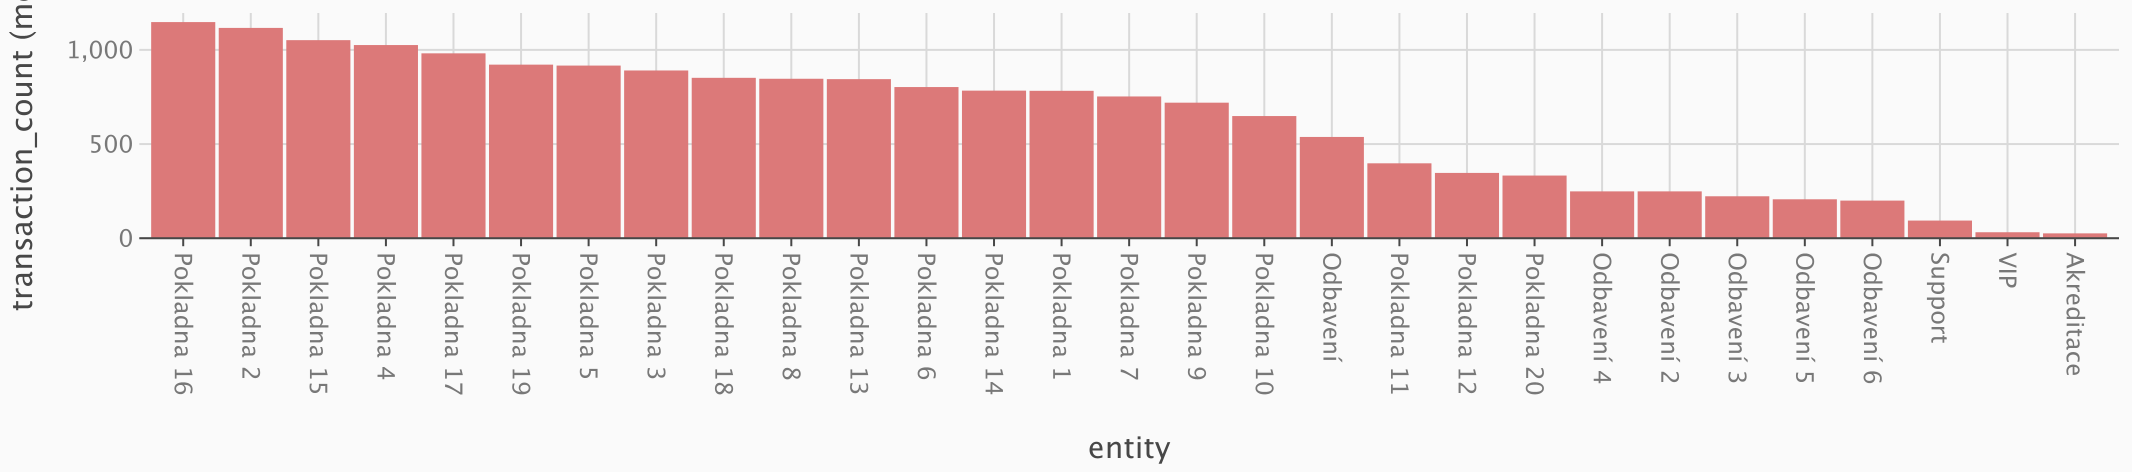
\includegraphics[width=\textwidth]{\ChartsDir/rq9-best-topup-points}
	\caption{\rqshorttext{performance-best-top-up-points} Best Top-Up Points}
	\label{chart:best-topup-points}
	\source
\end{chart}

Especially the \textbf{Odbavení} point processed only~\bfmtnum{529}~transactions but peaked at~\bfmtnum{125}~transactions per hour, which was much higher than the other check-in points and even higher than the best top-up points.

\begin{keytakeaways}
	\begin{itemize}
		\item The most busy top-up points are processed around~\bfmtnum{1000}~transactions during the event.
		\item The average peak of the top-up points was around~\bfmtnum{100}~transactions per hour.
		\item The least busy top-up points were the specific ones, such as the Support tent, VIP, and Accreditation points.
		\item Check-in points were less busy than the top-up points, but the \textbf{Odbavení} point peaked at~\bfmtnum{125}~transactions per hour.
	\end{itemize}
\end{keytakeaways}

\pagebreak[4]
%%% Performance / Best Sale Places, Top-Up Points, Vendors, and Products Analysis / Best Sale Places
%%% --------------------------------------------------------------

\subsubsection{Best Sale Places}
\label{subsubsec:analysis-best-sale-points}

The next focus will be on the best sale places, which are determined by the most orders created.

\makerqbox{performance-best-sale-points}

The process of finding the best sale places was similar to the previous one, but this time it required finding all sales transactions and their respective places.

Out of the total of~\bfmtnum{145}~sale places, the best place was undeniable the \textbf{L20 PIVNÍ STAN 1} with a total of~\bfmtnum{10114}~orders processed and the maximum peak of~\bfmtnum{840}~orders per hour.

Another interesting fact is the number of unique users processed at the places.
The \textbf{L20 PIVNÍ STAN 1} processed~\bfmtnum{9159}~unique customers, accounting for a significant portion (\bfmtnump[2]{91.50}{}\%) of the total\footnote{The total number of unique customers was found to be~\bfmtnum{10009}, which is more described in later sections}.

\begin{table}[htbp]
	\centering
	\small
	% @formatter:off
	\begin{tabularx}{\textwidth}{
		|>{\columncolor{unicorn_blue!5}\centering\arraybackslash}p{1cm}
		|>{\columncolor{unicorn_blue!5}\raggedright\arraybackslash}X
		|>{\columncolor{unicorn_blue!5}\raggedleft\arraybackslash}p{2.5cm}
		|>{\columncolor{unicorn_blue!5}\raggedleft\arraybackslash}p{2.5cm}
		|>{\columncolor{unicorn_blue!5}\raggedleft\arraybackslash}p{2.5cm}|}
		\hline
		\rowcolor{unicorn_blue}
		\textbf{}
		& \textbf{\color{white}Sale Point}
		& \textbf{\color{white}Customers}
		& \textbf{\color{white}Orders}
		& \textbf{\color{white}Max orders./h}
		\\\hline\hline
		% first rows
		\csvreader[
		head to column names,
		late after line={\\\hline},
		filter={\thecsvinputline<9}
		]{\DataDir/rq8-best-sale-points.csv}{
			entity=\colentity,
			customer_count=\colcustomers,
			transaction_count=\coltrxcount,
			max_hourly_peak=\colhourlypeak
		}{
			\the\numexpr\thecsvinputline-1
			& \colentity
			& \num[group-separator={,}]{\colcustomers}
			& \num[group-separator={,}]{\coltrxcount}
			& \num[group-separator={,}]{\colhourlypeak}
		}
		% separator
		\noalign{\vspace{1mm}}
		\multicolumn{5}{c}{\footnotesize{\textellipsis}}
		\\
		\noalign{\vspace{1mm}}
		\hline
		% last rows
		\csvreader[
		head to column names,
		late after line={\\\hline},
		filter={\thecsvinputline>132}
		]{\DataDir/rq8-best-sale-points.csv}{
			entity=\colentity,
			customer_count=\colcustomers,
			transaction_count=\coltrxcount,
			max_hourly_peak=\colhourlypeak
		}{
			\the\numexpr\thecsvinputline-1
			& \colentity
			& \num[group-separator={,}]{\colcustomers}
			& \num[group-separator={,}]{\coltrxcount}
			& \num[group-separator={,}]{\colhourlypeak}
		}
	\end{tabularx}
	% @formatter:on
	\caption{\rqshorttext{performance-best-sale-points} Best Sale Places}
	\label{tab:best-sale-points}
	\source
\end{table}

Based on this particular finding, we can assume that in the following analysis - the best vendors and products - the product preferences will be highly in favor of the beer beverages.
And thus the best vendor will probably be the organizer, as they sold all the beer beverages at the festival.

\begin{keytakeaways}
	\begin{itemize}
		\item The best sale place was the \textbf{L20 PIVNÍ STAN 1} with total~\bfmtnum{10114}~orders processed (\bfmtnump[2]{9.12}\%~of the total orders created).
		\item This place peaked at~\bfmtnum{840}~orders processed per hour.
		\item This place also processed~\bfmtnum{9159}~unique customers, which was~\bfmtnump[2]{91.50}\% of all active customers.
	\end{itemize}
\end{keytakeaways}

In conclusion to these two questions, the results show clearly the busiest points of the festival and their ability to handle the load.
However, the results can be visualized in a more interactive way, which would provide a better understanding of the data.

One especially interesting visualization of the best sale places and top-up points would be a heatmap of the festival area with the places and their respective transaction counts.
As this was initially intended to be part of the analysis, it was unfortunately not possible to create it due to the lack of the necessary data.

%%% Performance / Best Sale Places, Top-Up Points, Vendors, and Products Analysis / Best Vendors
%%% --------------------------------------------------------------

\subsubsection{Best Vendors}
\label{subsubsec:analysis-best-vendors}

To analyze the best vendors, in terms of performance, the same approach as with the sale places is used.

\makerqbox{performance-best-vendors}

The results in~\autoref{tab:best-vendors} below show the distribution of the processed orders over the vendors.

\begin{table}[htbp]
	\centering
	\small
	% @formatter:off
	\begin{tabularx}{\textwidth}{
		|>{\columncolor{unicorn_blue!5}\centering\arraybackslash}p{1cm}
		|>{\columncolor{unicorn_blue!5}\raggedright\arraybackslash}X
		|>{\columncolor{unicorn_blue!5}\raggedleft\arraybackslash}p{2.5cm}
		|>{\columncolor{unicorn_blue!5}\raggedleft\arraybackslash}p{2.5cm}|}
		\hline
		\rowcolor{unicorn_blue}
		\textbf{}
		& \textbf{\color{white}Vendor}
		& \textbf{\color{white}Customers}
		& \textbf{\color{white}Orders}
		\\\hline\hline
		% first rows
		\csvreader[
		head to column names,
		late after line={\\\hline},
		filter={\thecsvinputline<9}
		]{\DataDir/rq10-best-vendors.csv}{
			legal_name=\colentity,
			customer_count=\colcustomers,
			transaction_count=\coltrxcount,
		}{
			\the\numexpr\thecsvinputline-1
			& \colentity
			& \num[group-separator={,}]{\colcustomers}
			& \num[group-separator={,}]{\coltrxcount}
		}
		% separator
		\noalign{\vspace{1mm}}
		\multicolumn{5}{c}{\footnotesize{\textellipsis}}
		\\
		\noalign{\vspace{1mm}}
		\hline
		% last rows
		\csvreader[
		head to column names,
		late after line={\\\hline},
		filter={\thecsvinputline>25}
		]{\DataDir/rq10-best-vendors.csv}{
			legal_name=\colentity,
			customer_count=\colcustomers,
			transaction_count=\coltrxcount,
		}{
			\the\numexpr\thecsvinputline-1
			& \colentity
			& \num[group-separator={,}]{\colcustomers}
			& \num[group-separator={,}]{\coltrxcount}
		}
	\end{tabularx}
	% @formatter:on
	\caption{\rqshorttext{performance-best-vendors} Best Vendors}
	\label{tab:best-vendors}
	\source
\end{table}

As predicted in the previous section, the best vendor was the organizer, which processed the most orders and customers.
The total of~\bfmtnum{89217}~orders was processed by the organizer, which was~\bfmtnump[2]{80.04}\% of the total orders created and served~\bfmtnum{9831}~unique customers, which was~\bfmtnump[2]{98.22}\% of all active customers.

The second-best vendor, out of~\bfmtnum{27}~total, was some \textbf{Seller 05} with a huge difference of about~\bfmtnum{84104} orders less than the Organizer.

In these results, we did not go after the hourly maximums, as in the previous questions, as the vendors were not time-bound and could have been at multiple places simultaneously.
The results would not be so relevant and would not provide any additional insights.

\begin{keytakeaways}
	\begin{itemize}
		\item The best vendor was Organizer, who processed~\bfmtnum{89217}~orders (\bfmtnump[2]{80.04}\%~of the total orders).
		\item They~\bfmtnum{9831}~unique customers (\bfmtnump[2]{98.22}\%~of all active customers).
		\item The second-best vendor was behind around~\bfmtnum{84104}~orders less than the Organizer.
	\end{itemize}
\end{keytakeaways}

%%% Performance / Best Sale Places, Top-Up Points, Vendors, and Products Analysis / Best Products
%%% --------------------------------------------------------------

\subsubsection{Best Products}
\label{subsubsec:analysis-best-products}

The last focus will be on the best products, which are the products that were sold the most during the event.
However, unlike in the previous questions, this analysis should focus on product count sold, not the transaction count, since one order could have contained multiple products.

\makerqbox{performance-best-products}

Previously, the best products were predicted to be the beer beverages, as the organizer sold all the beer beverages at the festival.

The results in~\autoref{tab:best-products} below somehow confirm this prediction as the very best product was a returnable cup – \textbf{Kelímek – záloha} and the next several best products were beer beverages:

\begin{table}[htbp]
	\centering
	\small
	% @formatter:off
	\begin{tabularx}{\textwidth}{
		|>{\columncolor{unicorn_blue!5}\centering\arraybackslash}p{1cm}
		|>{\columncolor{unicorn_blue!5}\raggedright\arraybackslash}X
		|>{\columncolor{unicorn_blue!5}\raggedleft\arraybackslash}p{2.5cm}
		|>{\columncolor{unicorn_blue!5}\raggedleft\arraybackslash}p{2.5cm}
		|>{\columncolor{unicorn_blue!5}\raggedleft\arraybackslash}p{2.5cm}|}
		\hline
		\rowcolor{unicorn_blue}
		\textbf{}
		& \textbf{\color{white}Product}
		& \textbf{\color{white}Sales}
		& \textbf{\color{white}Refunds}
		& \textbf{\color{white}Customers}
		\\\hline\hline
		% first rows
		\csvreader[
		head to column names,
		late after line={\\\hline},
		filter={\thecsvinputline<9}
		]{\DataDir/rq11-best-products.csv}{
			product_name=\colproduct,
			customer_count=\colcustomers,
			sales_count=\colsalescount,
			refund_count=\colrefundcount
		}{
			\the\numexpr\thecsvinputline-1
			& \colproduct
			& \num[group-separator={,}]{\colsalescount}
			& \num[group-separator={,}]{\colrefundcount}
			& \num[group-separator={,}]{\colcustomers}
		}
		% separator
		\noalign{\vspace{1mm}}
		\multicolumn{5}{c}{\footnotesize{\textellipsis}}
		\\
		\noalign{\vspace{1mm}}
		\hline
		% last rows
		\csvreader[
		head to column names,
		late after line={\\\hline},
		filter={\thecsvinputline>326}
		]{\DataDir/rq11-best-products.csv}{
			product_name=\colproduct,
			customer_count=\colcustomers,
			sales_count=\colsalescount,
			refund_count=\colrefundcount
		}{
			\the\numexpr\thecsvinputline-1
			& \colproduct
			& \num[group-separator={,}]{\colsalescount}
			& \num[group-separator={,}]{\colrefundcount}
			& \num[group-separator={,}]{\colcustomers}
		}
	\end{tabularx}
	% @formatter:on
	\caption{\rqshorttext{performance-best-products} Best Products}
	\label{tab:best-products}
	\source
\end{table}

As there were more than \bfmtnum{300}~unique products sold during the event, a better visualization of the results would be a bar chart showing the best product categories instead of individual products.
This can be seen in~\autoref{chart:best-product-category} below.

\begin{chart}[h]
	\centering
	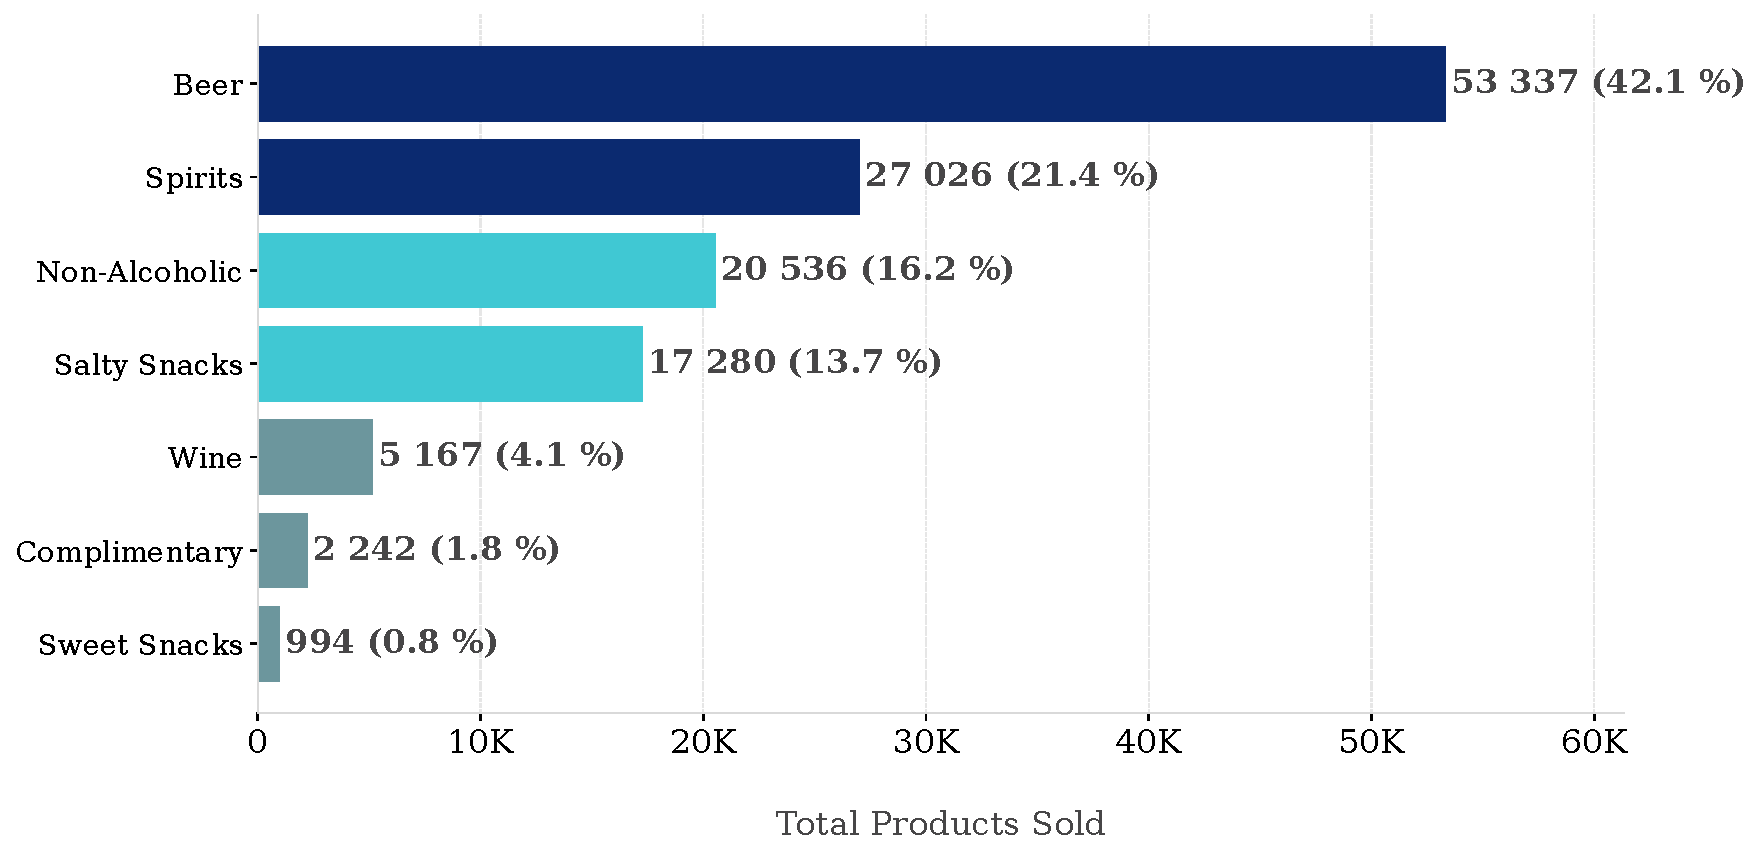
\includegraphics[width=\textwidth]{\ChartsDir/rq11-best-product-category}
	\caption{\rqshorttext{performance-best-products} Best Products by Category}
	\label{chart:best-product-category}
	\source
\end{chart}

This chart now confirms the prediction about the beer beverages, as the \textbf{Beer} category was the most sold during the event with a little more than~\bfmtnum{53000}~sold products.

\begin{keytakeaways}
	\begin{itemize}
		\item The best product was a returnable cup followed by several beer beverages.
		\item Prediction about the beer beverages was confirmed, as the \textbf{Beer} category was the most sold during the event.
	\end{itemize}
\end{keytakeaways}

This last analysis provided insights into the best products, which confirmed the previous predictions and will now serve as a basis for the next section, where the beverage consumption will be analyzed.

%%% Performance / Summary
%%% --------------------------------------------------------------

\subsection{Summary}
\label{subsec:analysis-performance-indicators-summary}

Thanks to this section, the performance indicators of the event were analyzed, and the key metrics were identified.
The results analyzed the transactional processing performance, identified several peak points during the event, and provided insights into the best sale places, top-up points, vendors, and products.
Providing a better understanding of the event's performance and giving more context for the next analysis dealing with the beverage consumption.


\pagebreak[4]

%%% Section: Beverage Consumption Analysis
%%% --------------------------------------------------------------


\section{Beverage Consumption Analysis}
\label{sec:analysis-beverage-consumption}

This section provides a detailed analysis of beverage consumption, which was previously determined to be the most important aspect of the event.

It should provide insights into overall consumption, as well as detailed information on returnable cups, the most popular beverages, and the leading beverage brands, while also answering the previously stated questions.

This section will address the next six research questions, after a minor logical reorganization into three groups:
\begin{enumerate}
	\item \fullref{subsec:analysis-beverage-returnable-cups}
	\item \fullref{subsec:analysis-beverage-total-consumption}
	\item and~\fullref{subsec:analysis-beverage-popular-brands}.
\end{enumerate}

%%% Beverage / Returnable Cups Analysis
%%% --------------------------------------------------------------

\subsection{Returnable Cups Analysis}
\label{subsec:analysis-beverage-returnable-cups}

Due to the little alteration of the local database and the previously referenced data in~\autoref{subsec:data-methodology-local-database-modifications}, it became possible to monitor the returnable cups and their associated transactions.

This capability, previously absent, should enhance comprehension of product sales and the utilization of returnable cups.

\makerqbox{beverage-returnable-cups}

To chart out the results, it was essential to analyze the actual contents of the transactions rather than merely identifying transactions including returnable cups,
as a single transaction may encompass many products and hence multiple returnable cups\footnote{The cups were sold for a price of~\fmtczk{70} with a~\fmtnum{21}\% VAT}.

Upon calculating the total number of issued and returned cups, the results depicted in~\autoref{chart:returnable-cups}~below illustrate the distribution of returnable cups throughout the event.

\begin{chart}[h]
	\centering
	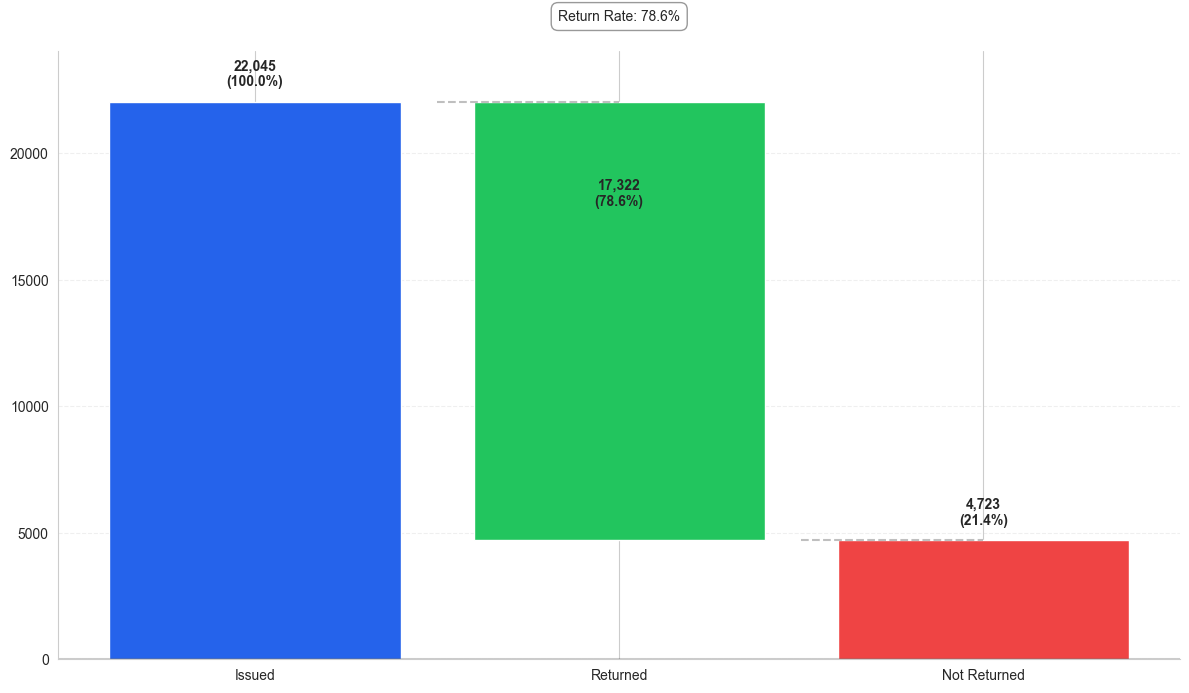
\includegraphics[width=\textwidth]{\ChartsDir/rq13-returnable-cups}
	\caption{\rqshorttext{beverage-returnable-cups} Returnable Cups}
	\label{chart:returnable-cups}
	\source
\end{chart}

The data indicate that a total of~\bfmtnum{20045}~cups was distributed during the event, with only~\bfmtnum{17322}~cups returned, yielding a return rate of~\bfmtnump[2]{78.60}\%.

This, however, does not imply that the remaining~\bfmtnum{4723}~cups were lost or regarded as a loss, as the cups were paid for and could have been retained as souvenirs by the customers.

\begin{keytakeaways}
	\begin{itemize}
		\item The total of~\bfmtnum{20045}~cups were issued during the festival.
		\item Only~\bfmtnum{17322}~cups returned resulted in a~\bfmtnump[2]{78.60}\%~return rate.
	\end{itemize}
\end{keytakeaways}

%%% Beverage / Total Consumption Analysis
%%% --------------------------------------------------------------

\subsection{Total Consumption Analysis}
\label{subsec:analysis-beverage-total-consumption}

This part focuses on the overall beverage consumption during the event.
Again, thanks to local database modifications, it was possible to track the beverage consumption easily, as each product now had a volume attribute in milliliters.

\makerqbox{beverage-total-consumption}

To find the results was quite straightforward, as it only required summing up the volumes of all sold products.

However, to present the results, it was convenient to group the products into categories and show the total consumption of each category and thus answering also the next question~\rqshort{beverage-popular-category}.

\makerqbox{beverage-popular-category}

These results are shown in~\autoref{tab:beverage-total-consumption} below and show a total of~\bfmtnum{37430}~liters of beverages consumed during the event, with the beer category being the most consumed.

\begin{table}[htbp]
	\centering
	% @formatter:off
	\begin{tabularx}{\textwidth}{|>{\columncolor{unicorn_blue!5}}X|>{\columncolor{unicorn_blue!5}}r|>{\columncolor{unicorn_blue!5}}r|}
		\hline
		\rowcolor{unicorn_blue}
		\textbf{\color{white}Beverage Category}
		& \textbf{\color{white}Volume}
		& \textbf{\color{white}Ratio}
		\\
		\hline
		\hline
		\colorindicator{1}Beer & \fmtnump[2]{25883.3}~l & \fmtnump[2]{69.15}~\% \\
		\colorindicator{2}Non-alcoholic & \fmtnump[2]{7832.47}~l & \fmtnump[2]{20.92}~\% \\
		\colorindicator{3}Spirits / other alcohol & \fmtnump[2]{2842.14}~l & \fmtnump[2]{7.59}~\% \\
		\colorindicator{4}Wine & \fmtnum{872.58}~l & \fmtnump[2]{2.34}~\% \\
		\hline
		\textbf{Total volume} & \bfmtnump[2]{37430.49}~l & \fmtnum{100}~\% \\
		\hline
	\end{tabularx}
	% @formatter:on
	\caption{\rqshorttext{beverage-total-consumption} Total Beverage Consumption}
	\label{tab:beverage-total-consumption}
	\source
\end{table}

These results serve as a basis for the next questions, which focuses on the most consumed beverage brands rather than product categories.

\begin{keytakeaways}
	\begin{itemize}
		\item A total of~\bfmtnum{37430}~liters of beverages were consumed during the event.
		\item The beer category was the most consumed with~\bfmtnum{25883}~liters consumed.
	\end{itemize}
\end{keytakeaways}

%%% Beverage / Popular Brands Analysis
%%% --------------------------------------------------------------

\subsection{Popular Brands Analysis}
\label{subsec:analysis-beverage-popular-brands}

This section explores beverage preferences, concentrating on the most popular brands within the leading categories: \fullref{subsubsec:analysis-beverage-popular-beer}, \fullref{subsubsec:analysis-beverage-popular-non-alcoholic}, \fullref{subsubsec:analysis-beverage-popular-alcoholic}.

Answering these questions required the identification and categorization of all beverage products, followed by the computation of their overall consumption.
However, this was not entirely easy, as the products were not uniformly labeled.
This indicated that beers labeled as~\enquote{Radegast 10} and~\enquote{Radegast 12} were not categorized together, resulting in biased outcomes.

To address this issue, the products ought to be categorized by their brand rather than by their name.
This methodology seemed logical; nevertheless, the data lacked brand information, containing simply the product name.

A systematic approach would be to extend the database with brands and back-fill the products with a link to the brand.
This would require a significant amount of work and time, which was not available at the time of this analysis.

A more straightforward and manual method was used, wherein the product's~\enquote{brand} was identified by extracting the essential parts of the product name, eliminating redundant elements such as volume, beer grade, or other details.
This helped produce better results, however, still lack complete accuracy.

%%% Beverage / Popular Brands Analysis / Beer Brands Analysis
%%% --------------------------------------------------------------

\subsubsection{Beer Brands Analysis}
\label{subsubsec:analysis-beverage-popular-beer}
Starting with the most consumed and most popular category – beer.

\makerqbox{beverage-top-beer}

The results in~\autoref{chart:beverage-top-beer} below illustrate the distribution of the most consumed beer brands during the event.

\begin{chart}[H]
	\centering
	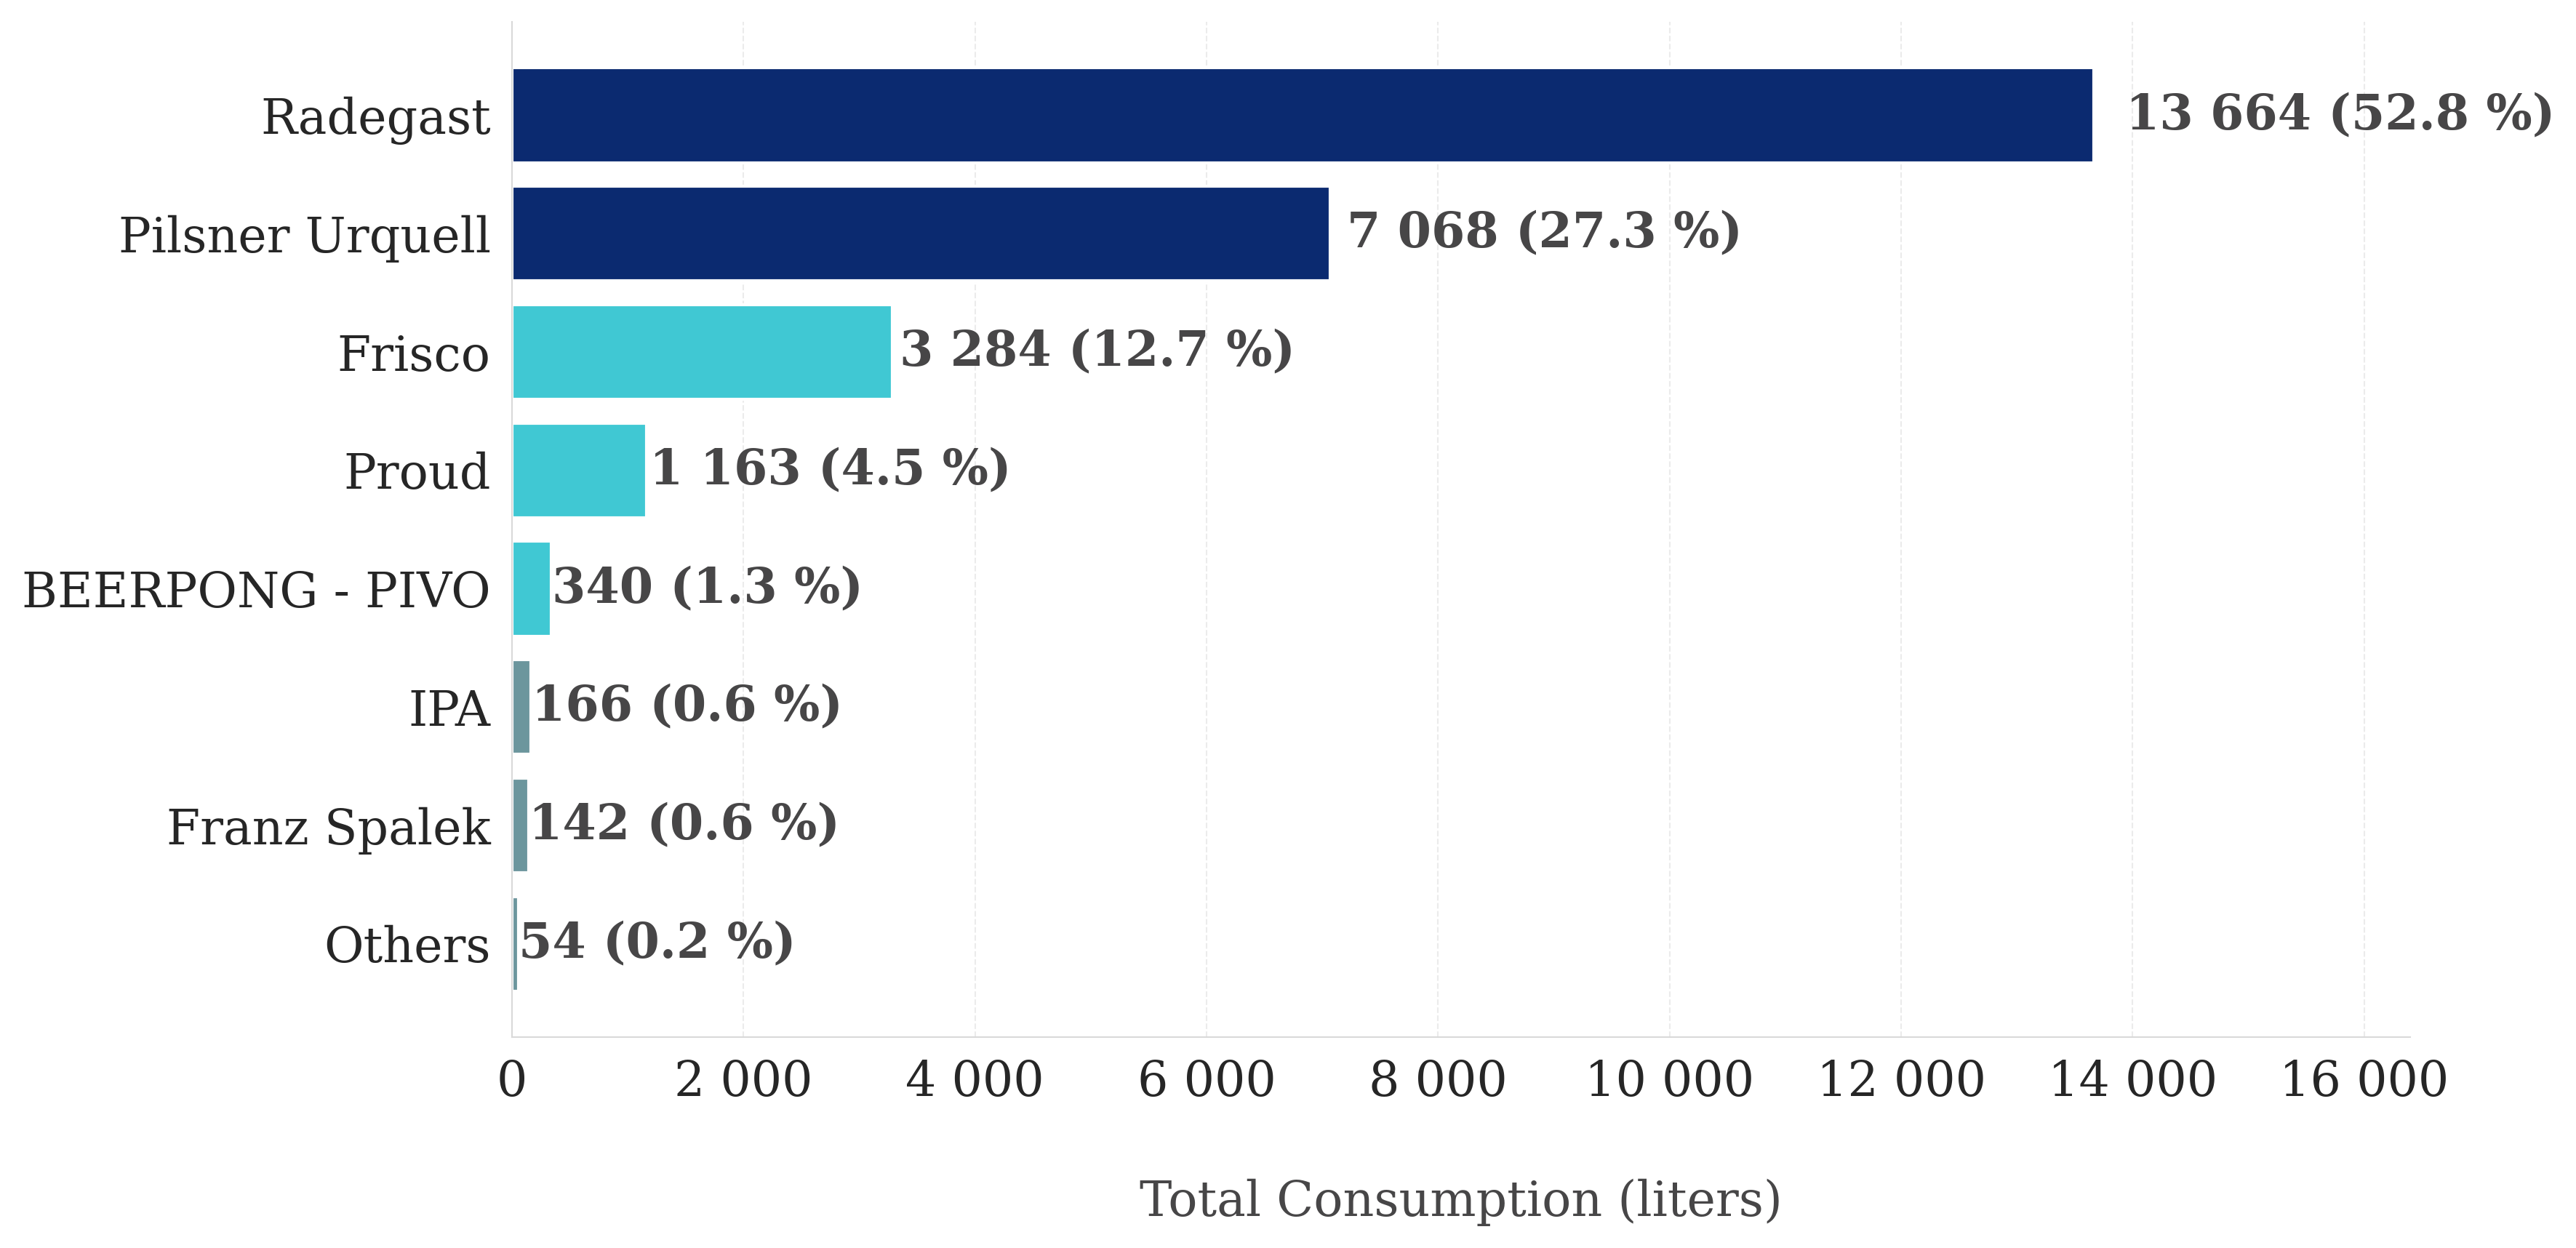
\includegraphics[width=\textwidth]{\ChartsDir/rq15-top-beer-brands}
	\caption{\rqshorttext{beverage-top-beer} Most Consumed Beer Brands}
	\label{chart:beverage-top-beer}
	\source
\end{chart}

This distribution indicates that the most consumed beer brand was \textbf{Radegast}, with a total consumption of~\bfmtnum{13665}~liters and~\bfmtnum{27329} units sold.

The second was \textbf{Pilsner Urquell}, which had half the consumption of \textbf{Radegast}, followed by the \textbf{Frisco} and \textbf{Proud} brands.
A complete list of all ten brands from the festival is shown in~\autoref{tab:beverage-top-beer}~below.

\begin{table}[H]
	\centering
	\small
	% @formatter:off
	\begin{tabularx}{\textwidth}{
		|>{\columncolor{unicorn_blue!5}\centering\arraybackslash}p{1cm}
		|>{\columncolor{unicorn_blue!5}\raggedright\arraybackslash}X
		|>{\columncolor{unicorn_blue!5}\raggedleft\arraybackslash}p{4cm}
		|>{\columncolor{unicorn_blue!5}\raggedleft\arraybackslash}p{2.5cm}|}
		\hline
		\rowcolor{unicorn_blue}
		\textbf{}
		& \textbf{\color{white}Beer brand}
		& \textbf{\color{white}Total consumption}
		& \textbf{\color{white}Units sold}
		\\\hline\hline
% rows
		\csvreader[
			head to column names,
			late after line={\\\hline},
		]{\DataDir/rq15-top-beer-brands.csv}{
			subcategory=\colbrand,
			total_consumption_liters=\colconsumption,
			transaction_count=\coltrxcount,
			total_sold=\colunits
		}{
			\the\numexpr\thecsvinputline-1
			& \colbrand
			& \num[group-separator={,}]{\colconsumption}~l
			& \num[group-separator={,}]{\colunits}
		}
		\hline
		\noalign{\vspace{1mm}}
		\hline
		\rowcolor{unicorn_blue!20}
		\textbf{}
		& \textbf{Total}
		& {\bfmtnum{19793}}~l
		& {\bfmtnum{53990}}
		\\\hline
	\end{tabularx}
	% @formatter:on
	\caption{\rqshorttext{beverage-top-beer} Most Consumed Beer Brands}
	\label{tab:beverage-top-beer}
	\source
\end{table}

The data demonstrate a strong preference for Radegast beer among festival attendees.
The price may have influenced this, as the Radegast was generally slightly less expensive than, for instance, the Pilsner Urquell\footnote{The price of Radegast ranged from~\fmtczk{60} to~\fmtczk{66} and Pilsner Urquell was priced at~\fmtczk{60} to~\fmtczk{75}, depending on the beer size and its grade}.

\begin{keytakeaways}
	\begin{itemize}
		\item The most consumed beer brand was \textbf{Radegast} with a total of~\bfmtnum{13665}~liters consumed.
		\item The second most consumed beer brand was the \textbf{Pilsner Urquell} with half the consumption of the Radegast.
	\end{itemize}
\end{keytakeaways}

\vspace*{\fill} % fill rest due to the foonote placement
\pagebreak[4]

%%% Beverage / Popular Brands Analysis / Non-alcoholic Brands Analysis
%%% --------------------------------------------------------------

\subsubsection{Non-alcoholic Brands Analysis}
\label{subsubsec:analysis-beverage-popular-non-alcoholic}

\makerqbox{beverage-top-non-alcoholic}

Aggregated similarly as in the previous analysis, the results in~\autoref{chart:beverage-top-non-alcoholic}~below show the distribution of the most consumed non-alcoholic brands during the event.

\begin{chart}[H]
	\centering
	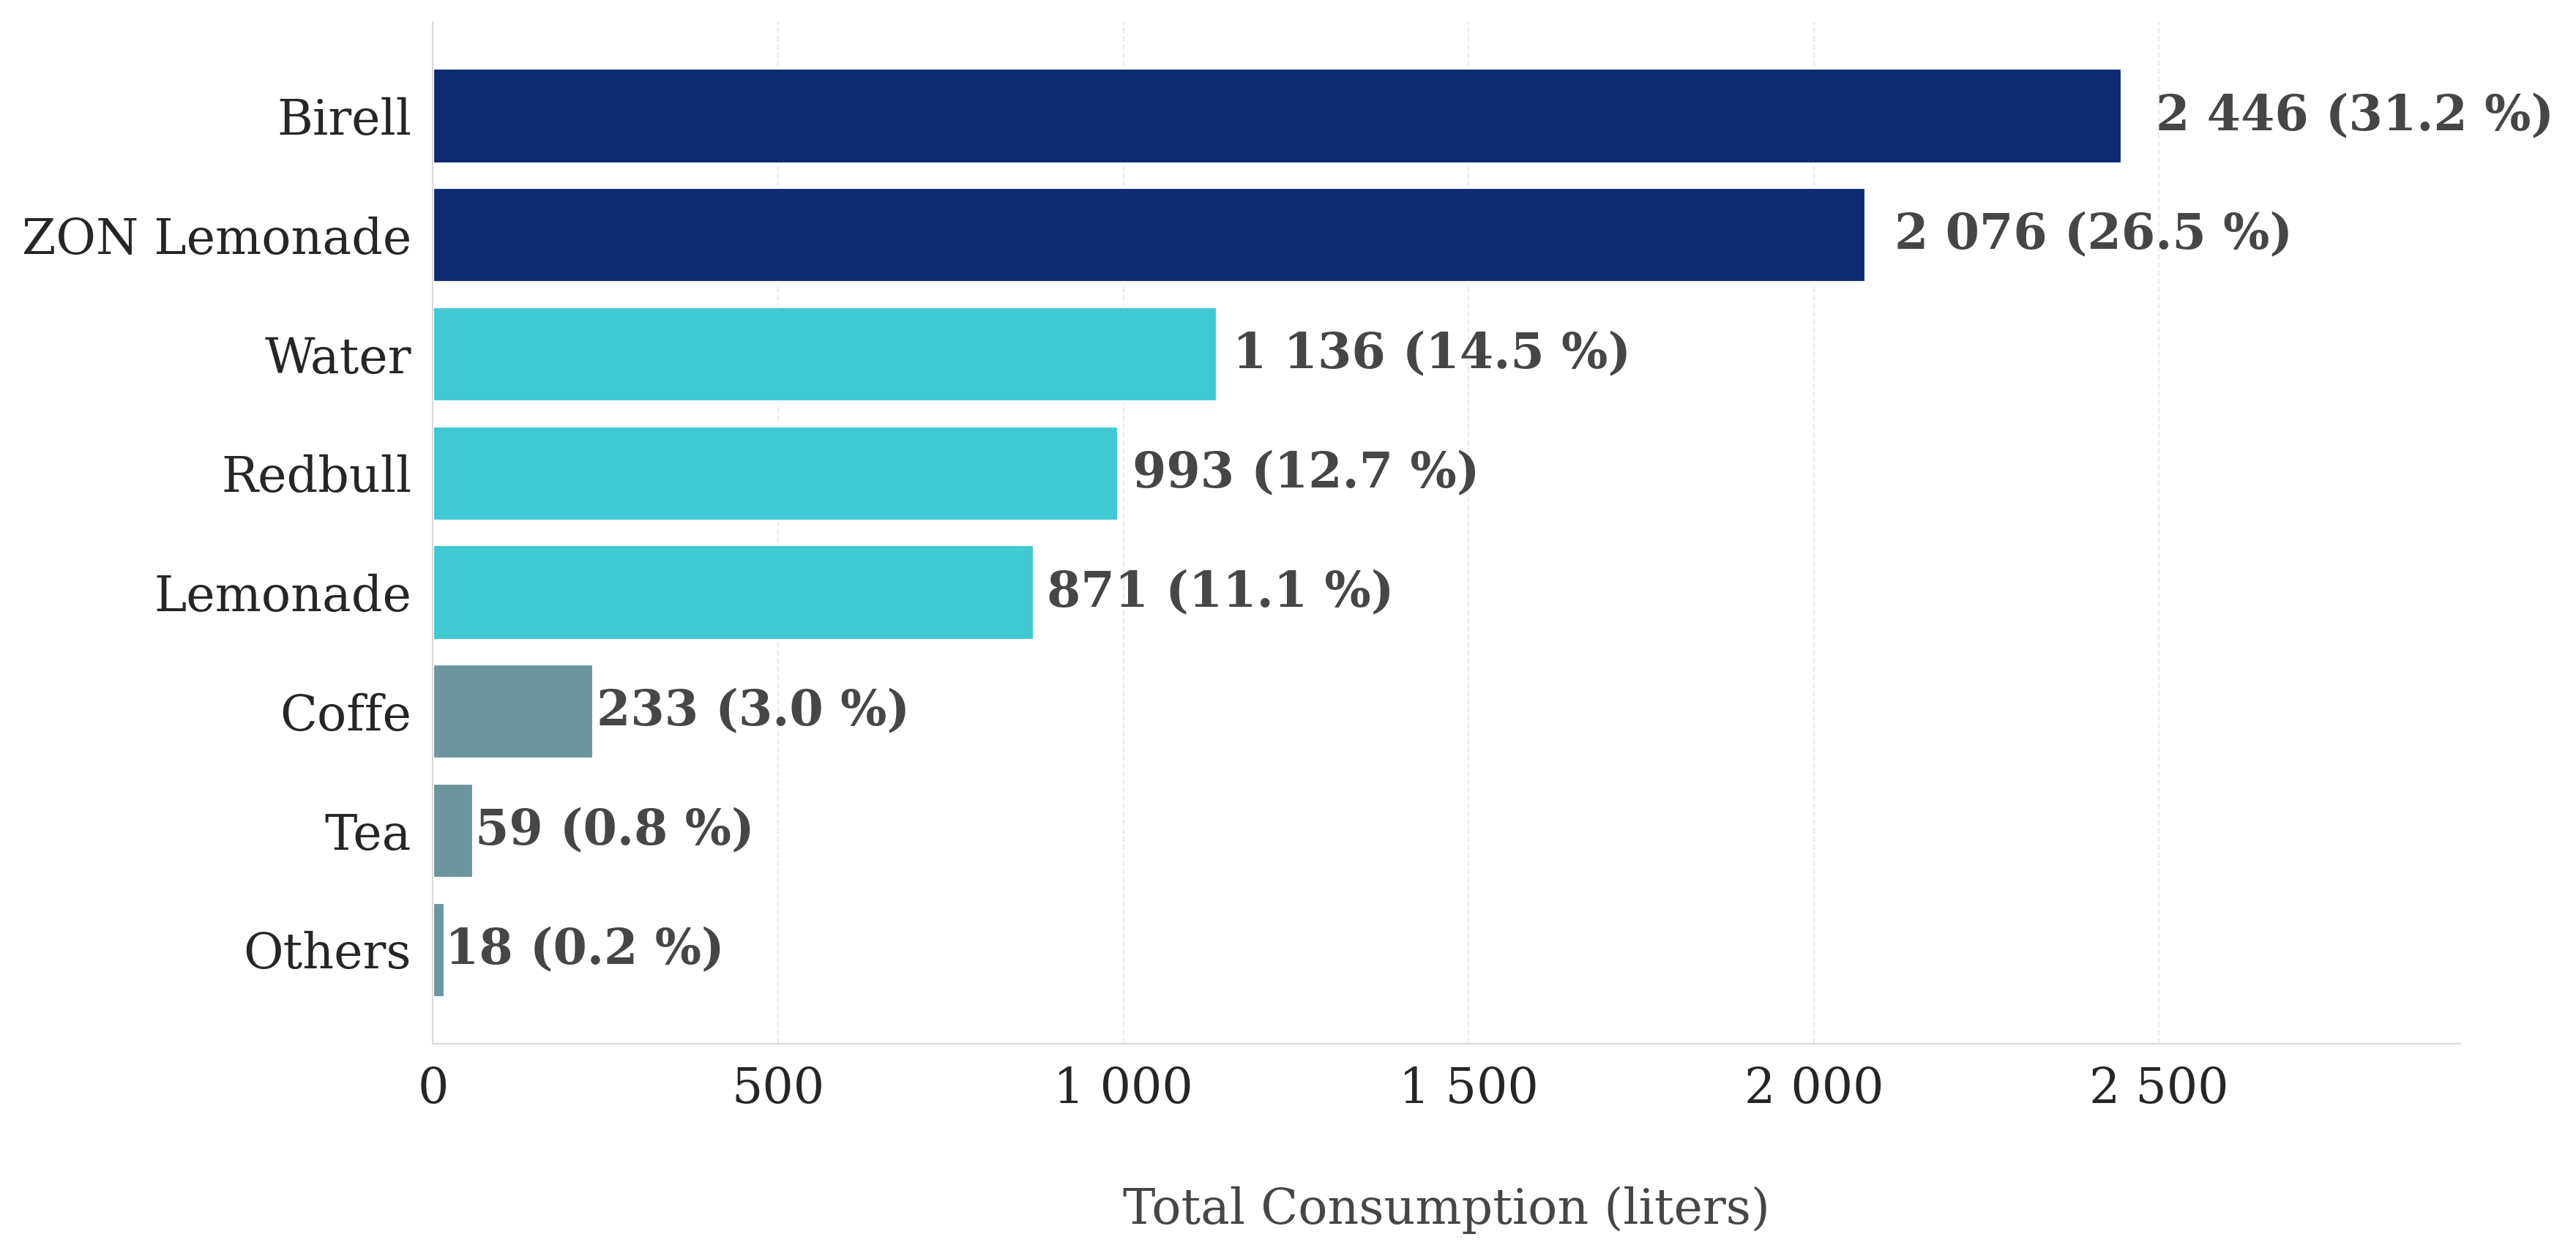
\includegraphics[width=\textwidth]{\ChartsDir/rq17-top-non-alco-brands}
	\caption{\rqshorttext{beverage-top-beer} Most Consumed Non-Alcoholic Brands}
	\label{chart:beverage-top-non-alcoholic}
	\source
\end{chart}

The results indicate a close rivalry between the \textbf{Birell} and \textbf{ZON Lemonade} brands, with Birell emerging as the most consumed non-alcoholic beverage at the event.
A total of~\bfmtnum{2446}~liters drank and~\bfmtnum{4893}~units sold established it as the most popular non-alcoholic beverage, taking over~\bfmtnum{31}\% of the total non-alcoholic consumption.

\begin{keytakeaways}
	\begin{itemize}
		\item The most consumed non-alcoholic brand was \textbf{Birell} with a total of~\bfmtnum{2446}~liters consumed.
		\item The second most consumed non-alcoholic brand was the \textbf{ZON Lemonade}.
	\end{itemize}
\end{keytakeaways}

%%% Beverage / Popular Brands Analysis / Alcoholic Brands Analysis
%%% --------------------------------------------------------------

\subsubsection{Alcoholic Brands Analysis}
\label{subsubsec:analysis-beverage-popular-alcoholic}

The last part of this section focuses on other alcoholic beverages, such as spirits, shots, cocktails, and other alcoholic beverages.

\makerqbox{beverage-top-alcoholic}

This analysis consisted of a total of 23 different brands consisting mostly of spirits and shots.
The results presented in this section may be more biased than the previous ones, as the brand determination was more challenging due to the lack of consistent labeling.
Moreover, previously it was necessary to classify the products with the volume information, which is not so straightforward for shots and spirits.

The results in~\autoref{chart:beverage-top-alcoholic}~indicate that the most consumed alcoholic brand was the \textbf{Absolut Vodka}.
With a total of~\bfmtnum{239}~liters consumed and~\bfmtnum{9177}~units sold, it was the most popular alcoholic beverage in terms of consumption.
The second most consumed brand was \textbf{Beefeater} with \bfmtnum{170}~liters consumed and a total count of~\bfmtnum{4628}~units sold.

\begin{chart}[H]
	\centering
	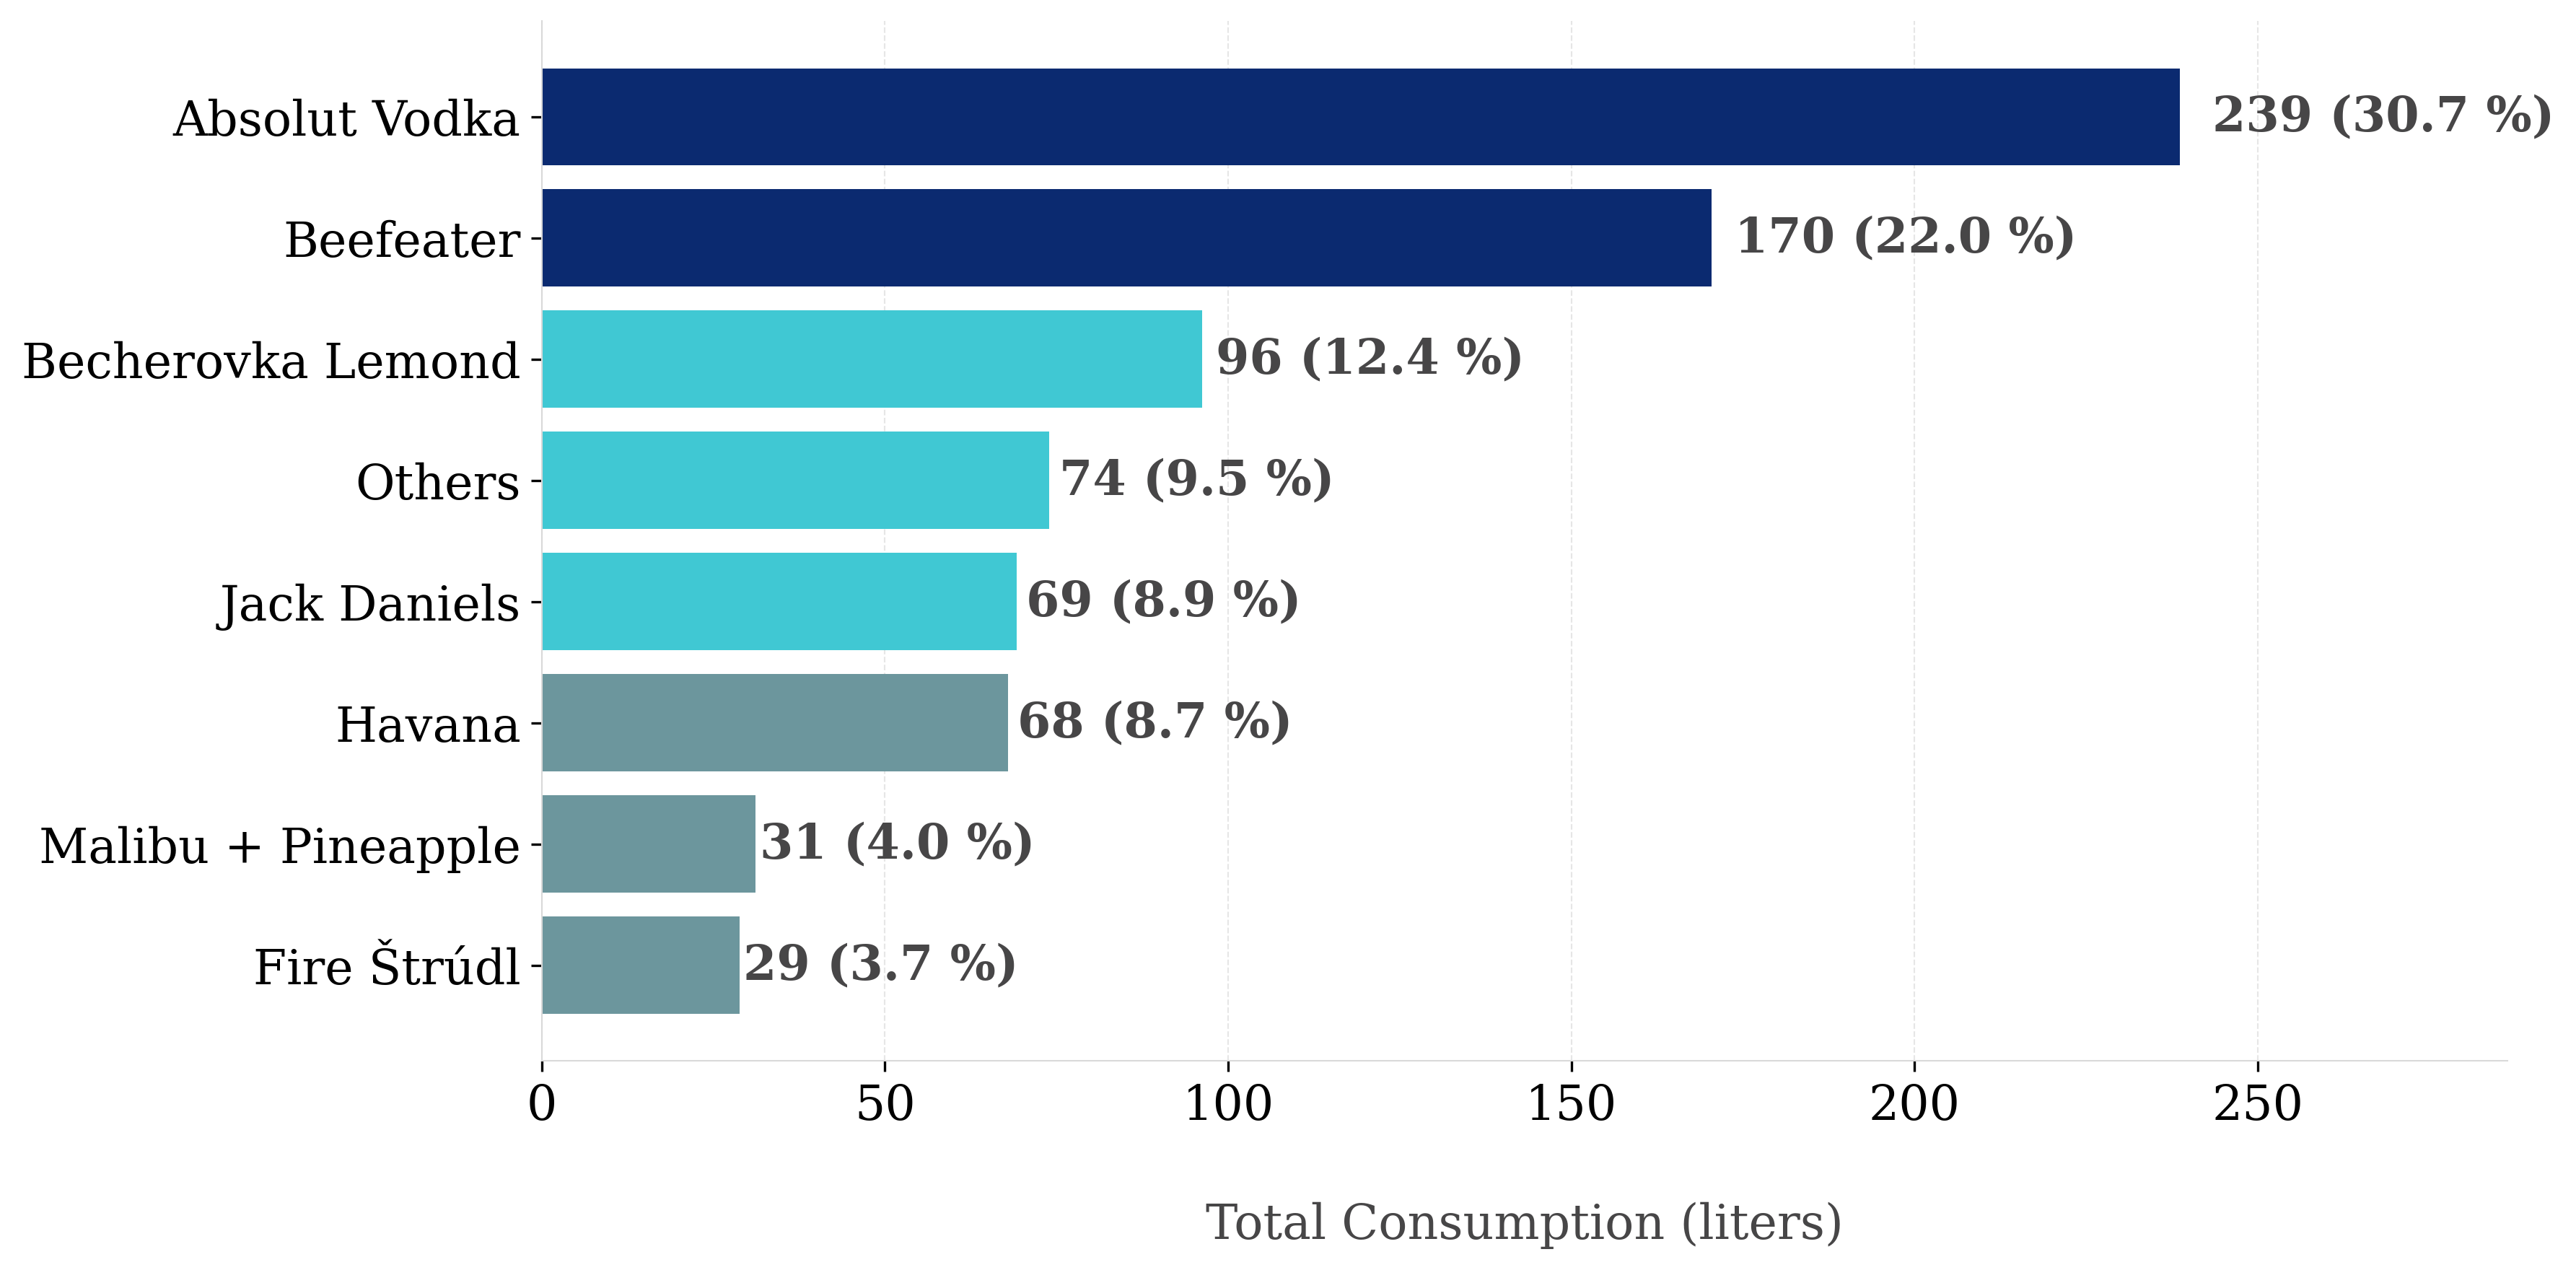
\includegraphics[width=\textwidth]{\ChartsDir/rq16-top-alco-brands}
	\caption{\rqshorttext{beverage-top-beer} Most Consumed Non-Alcoholic Brands}
	\label{chart:beverage-top-alcoholic}
	\source
\end{chart}

However, the results should be taken with caution, as the data may not be entirely accurate due to the previously mentioned issues.
The accuracy of back-filling the volume information for shots and spirits was not as high as for beer and non-alcoholic beverages.
Since shots and spirits are usually sold in various sizes, in combination with other beverages, the volume information was not always available or reliable.

\begin{keytakeaways}
	\begin{itemize}
		\item The most consumed alcoholic brand was \textbf{Absolut Vodka} with a total of~\bfmtnum{239}~liters consumed.
		\item The second most consumed alcoholic brand was the \textbf{Beefeater}.
		\item The results should still be taken with caution due to the uncertainty of the volume information in certain cases.
	\end{itemize}
\end{keytakeaways}


%%% Beverage / Summary
%%% --------------------------------------------------------------

\subsection{Summary}
\label{subsec:analysis-beverage-consumption-summary}

Insights into beverage consumption, covered in this section, should provide a better understanding of the overall preferences and total consumptions during the festival.
As this data was not previously available, it was a valuable addition to the analysis and will play a significant role when presenting the results to the festival organizers.

The results showed the total consumption of all beverages, the insightful view on returnable cups usage, and the most consumed beverage brands in the most popular categories.

With the data available, there are still many more questions that could be answered, particularly in combination with customer data.
However, clear bounds were set for this analysis to answer the most important questions asked by the festival organizers.


\pagebreak[4]
%%% Section: Customer Analysis
%%% --------------------------------------------------------------


\section{Customer Analysis}
\label{sec:analysis-customers}

This section will focus on customer analysis, which should provide interesting insights into festival attendees' behavior and segmentation.

Because the organizers lacked deeper insights into festival attendees, this analysis should contribute significantly to a better understanding of the event.

The analysis addresses the remaining research questions, which have been reorganized into four logical groups to improve the narrative flow:\\
\begin{enumerate}
	\item \fullref{subsec:analysis-customer-event-attendance-timeline}
	\item \fullref{subsec:analysis-customer-segmentation},
	\item \fullref{subsec:analysis-customer-payment-behavior}
	\item and~\fullref{subsec:analysis-customer-purchase-pattern}.
\end{enumerate}

%%% Customer / Event Attendance and Timeline Analysis
%%% --------------------------------------------------------------

\subsection{Event Attendance and Timeline Analysis}
\label{subsec:analysis-customer-event-attendance-timeline}

This section should provide information about attendees' initial behavior, total attendance throughout the festival, and later top-up behavior.

Before delving into the analysis, it was necessary to define the term \enquote{active customer} in this context.

\begin{infobox}{Definition of an Active Customer}
	An active customer is a customer identified by a chip wristband issued at the festival.
\end{infobox}

This definition was crucial for the analysis, as it allowed for the identification of unique customers and their behavior throughout the festival.
Although it cannot be guaranteed that the wristbands were not shared among attendees, or misused in any other way, the assumption was that the wristbands were used as intended.

\pagebreak[4]

%%% Customer / Event Attendance and Timeline Analysis / Total Attendance and Daily Activity
%%% --------------------------------------------------------------

\subsubsection{Total Attendance and Daily Activity}
\label{subsubsec:analysis-total-attendance}

\makerqbox{customers-total-attendance}

The analysis shows that the festival drew total~\bfmtnum{10009}~unique customers over the three-day period.
However, the daily attendance figures show interesting patterns in how these customers were distributed throughout the festival days.

Looking at the daily active customers:
\begin{itemize}
	\item Day 1 (Thursday):~\bfmtnum{6214}~active customers
	\item Day 2 (Friday):~\bfmtnum{5832}~active customers
	\item Day 3 (Saturday):~\bfmtnum{8066}~active customers
\end{itemize}

These numbers indicate that many customers attended multiple days of the festival, as the sum of daily attendees (\bfmtnum{20112}) is significantly higher than the unique customer count.
This was expected, as the festival was designed to attract visitors for multiple days.

The attendance peaked on the final day of the festival, with Day 2 showing slightly lower attendance than the opening day.
The significant increase in attendance on Day 3 suggests that the festival successfully attracted weekend visitors.

\begin{keytakeaways}
	\begin{itemize}
		\item Total of~\bfmtnum{10009}~unique customers over the three days.
		\item The highest attendance was on Day 3 (Saturday) with~\bfmtnum{8066}~active customers.
		\item Consistent attendance on weekdays (Days 1–2) with a slight decrease on Day 2.
		\item Significant increase in attendance (38\% higher than Day 2) for the weekend (Day 3).
	\end{itemize}
\end{keytakeaways}

%%% Customer / Event Attendance and Timeline Analysis / Visitor Arrival Patterns
%%% --------------------------------------------------------------

\subsubsection{Visitor Arrival Patterns}
\label{subsubsec:analysis-visitor-patterns}

\makerqbox{customers-new-visitors}

Before analyzing the visitor arrival patterns, it was necessary to define what a new visitor registration meant in this context.

\begin{infobox}{Definition of a New Visitor}
	A customer registration in this context means a new unique wristband issuance, which also, other than for payments, serves as an access pass to the festival in means of access control.
\end{infobox}

The analysis of visitor arrival patterns, shown in~\autoref{chart:visitor-arrival-patterns}, reveals distinct peak periods across the three festival days, with significant variations in the rate of new visitor registrations throughout each day.

\begin{chart}[h]
	\centering
	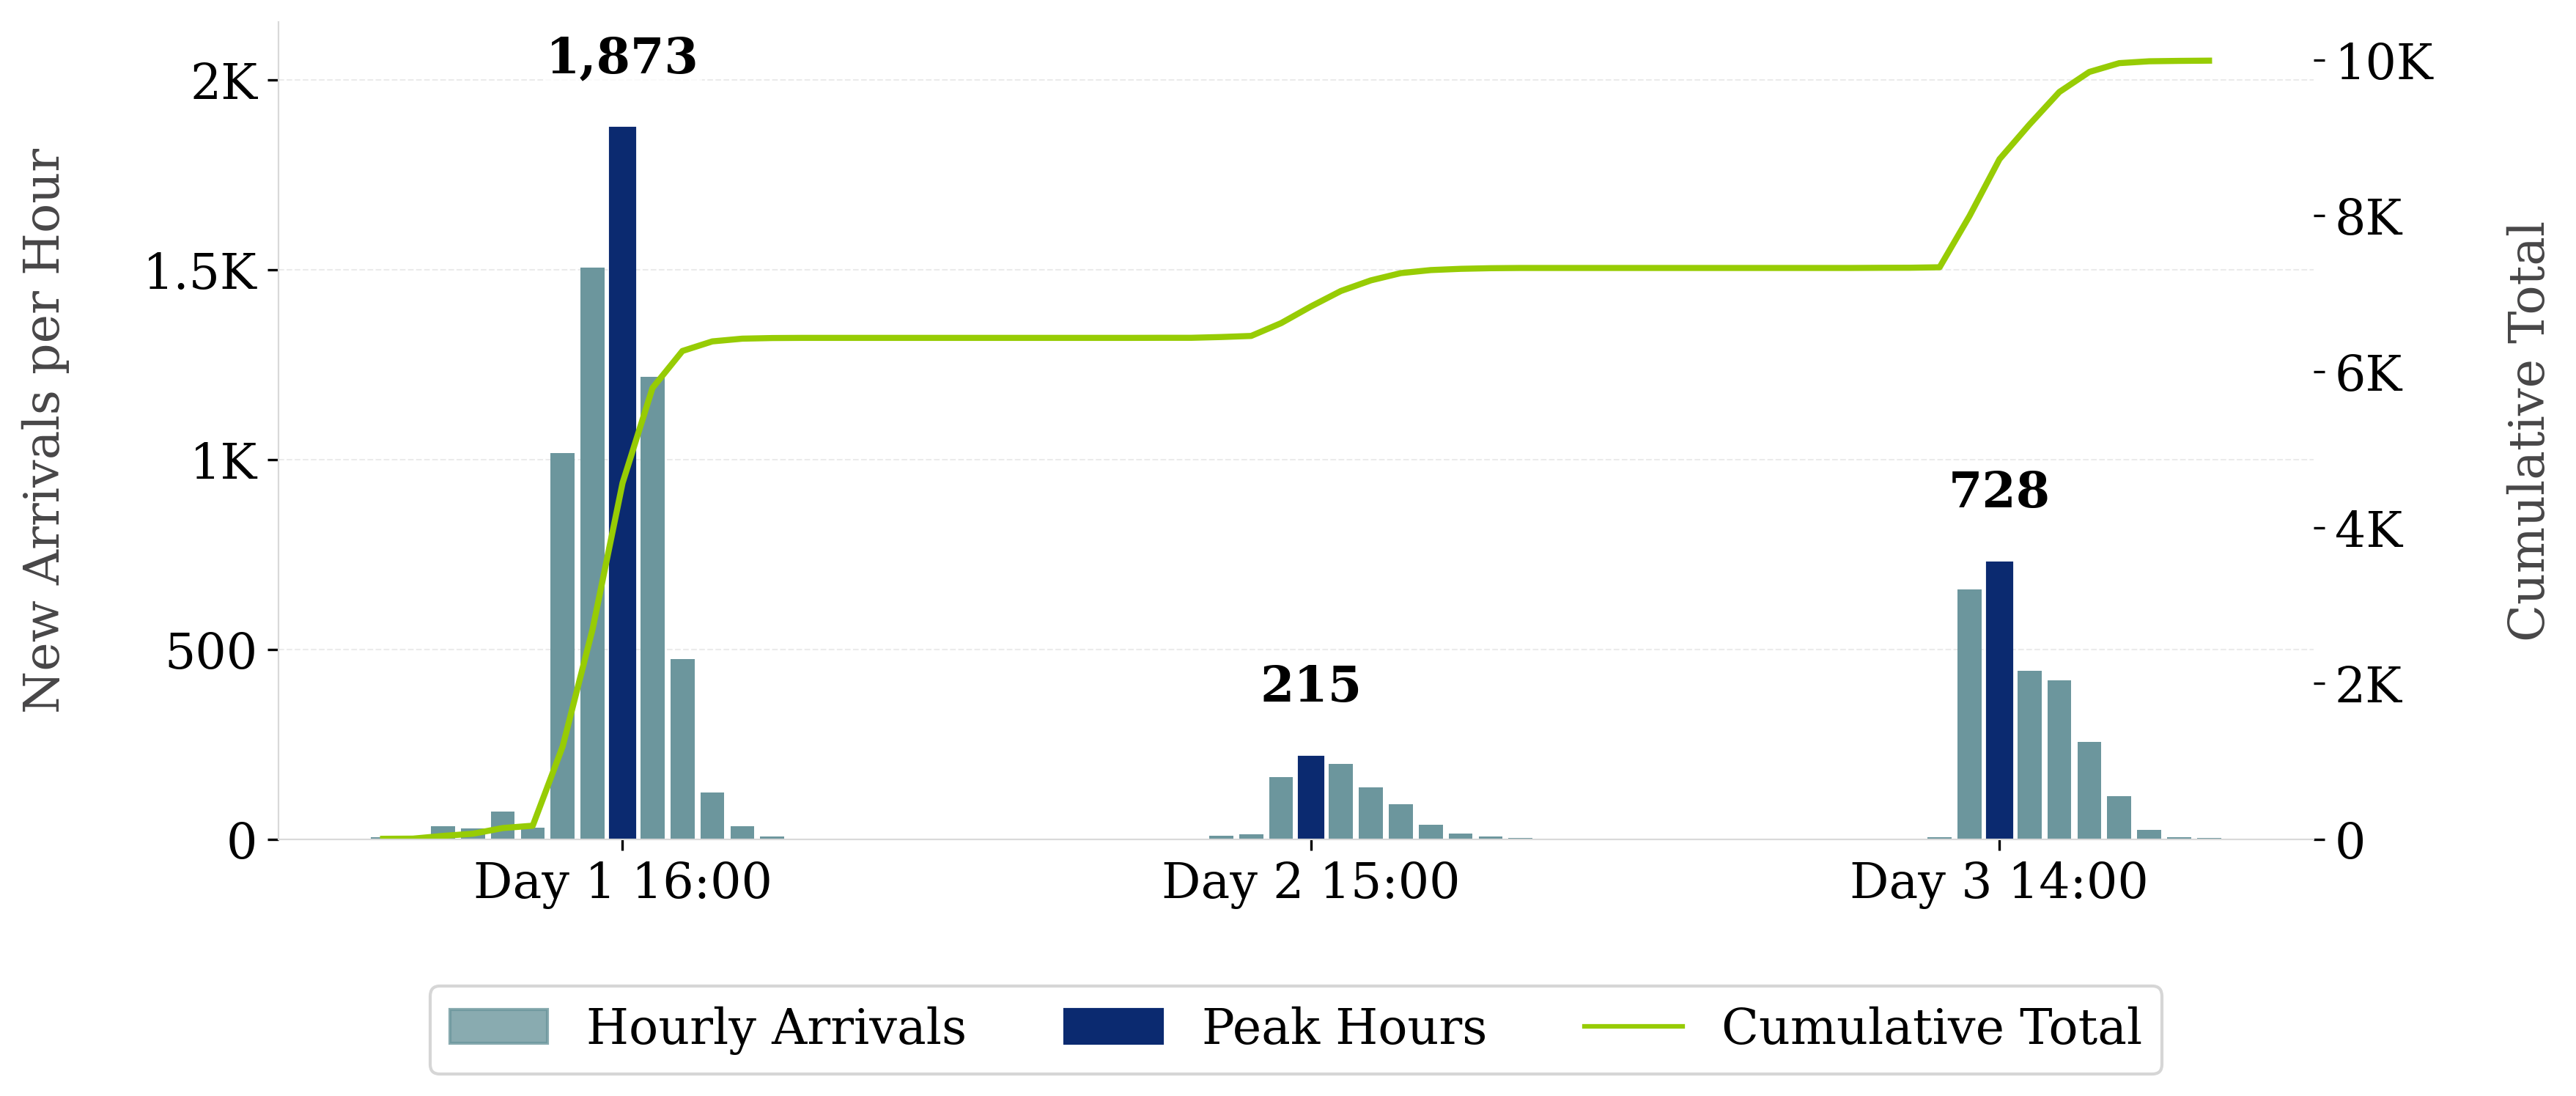
\includegraphics[width=\textwidth]{\ChartsDir/rq24-arrival-patterns}
	\caption{\rqshorttext{customers-new-visitors} Visitor Arrival Patterns}
	\label{chart:visitor-arrival-patterns}
	\source
\end{chart}

The data reveals three distinct patterns across the festival days:

\begin{itemize}
	\item \textbf{Day 1 (Thursday)}: A rapid peak of approximately~\bfmtnum{1873}~new visitors was observed during the 16:00 hour, which was the time of the highest arrival activity.
	The day showed a clear pattern of increasing arrivals from 14:00 to 16:00, followed by a gradual decline resulting in~\bfmtnum{6433}~new visitors.
	\item \textbf{Day 2 (Friday)}: A modest peak of~\bfmtnum{215}~visitors at 15:00, but significantly lower new arrivals than on Day 1.
	This decrease in the number of new arrivals was expected, as a significant number of visitors had already completed the registration process on Day 1.
	\item \textbf{Day 3 (Saturday)}: The surge of fresh arrivals, which peaked at~\bfmtnum{728} new visitors at 14:00, clearly reflected the weekend visitors.
\end{itemize}

The data indicates that the majority of visitor arrivals occurred during the afternoon hours (14:00–17:00) on all days.
Minimal new arrivals were consistently observed during the early morning hours (before 10:00) and late evening hours (after 20:00).

\begin{keytakeaways}
	\begin{itemize}
		\item Highest single-hour registration peak:~\bfmtnum{1873}~visitors (Day 1, 16:00).
		\item The registration window that was most effective was from 14:00 to 17:00 on all days.
		\item Day 1 accounted for approximately~\bfmtnump[2]{64.39}\%~of total arrivals.
		\item Weekend (Day 3) saw renewed registration activity with the peak of~\bfmtnum{728}~new visitors.
	\end{itemize}
\end{keytakeaways}

%%% Customer / Event Attendance and Timeline Analysis / Top-Up Peaks
%%% --------------------------------------------------------------

\subsubsection{Time to First Transaction}
\label{subsubsec:analysis-first-transaction}

\makerqbox{customers-visitor-time}

The analysis reveals significant variations in how quickly different types of visitors made their first transaction after arrival.
Overall, the average time to the first transaction was~\bfmtnum{79.55}~minutes.
However, this number alone is misleading, as evidenced by the much lower median of~\bfmtnum{7}~minutes and mode of~\bfmtnum{3}~minutes.

\begin{table}[htbp]
	\centering
	\small
	% @formatter:off
	\begin{tabularx}{\textwidth}{
		|>{\columncolor{unicorn_blue!5}\centering\arraybackslash}l
		|>{\columncolor{unicorn_blue!5}\raggedleft\arraybackslash}X
		|>{\columncolor{unicorn_blue!5}\raggedleft\arraybackslash}X
		|>{\columncolor{unicorn_blue!5}\raggedleft\arraybackslash}X
		|>{\columncolor{unicorn_blue!5}\raggedleft\arraybackslash}X|
	}
		\hline
		\rowcolor{unicorn_blue}
		\textbf{\color{white}Visitor Type}
		& \textbf{\color{white}Average}
		& \textbf{\color{white}Mode}
		& \textbf{\color{white}Median}
		& \textbf{\color{white}Max}
		\\
		\hline
		\colorindicator{1}Guest
		& \textbf{2}~h~\textbf{21}~min
		& \bfmtnum{0}~min
		& \bfmtnum{10}~min
		& \textbf{52}~h~\textbf{56}~min
		\\
		\colorindicator{2}Regular
		& \bfmtnum{44.68}~min
		& \bfmtnum{0}~min
		& \bfmtnum{6}~min
		& \textbf{47}~h~\textbf{32}~min
		\\
		\colorindicator{3}Online
		& \bfmtnum{66.85}~min
		& \bfmtnum{3}~min
		& \bfmtnum{7}~min
		& \textbf{44}~h~\textbf{51}~min
		\\
		\colorindicator{4}Staff
		& \textbf{9}~h~\textbf{44}~min
		& \bfmtnum{7}~min
		& \textbf{3}~h~\textbf{54}~min
		& \textbf{58}~h~\textbf{12}~min
		\\
		\hline
		\rowcolor{unicorn_blue!20}
		\textbf{Overall}
		& \bfmtnum{79.55}~min
		& \bfmtnum{3}~min
		& \bfmtnum{7}~min
		& \textbf{58}~h~\textbf{12}~min
		\\
		\hline
	\end{tabularx}
	% @formatter:on
	\caption{\rqshorttext{customers-visitor-time} Time to First Transaction}
	\label{tab:time-to-first-transaction}
	\source
\end{table}

Breaking down the analysis by visitor type\footnote{Visitor or rather, chip types are described in the~\fullref{tab:chip-types} table.}, reveals distinct patterns:
\begin{itemize}
	\item \textbf{Regular}: Quickest to transact, with an average of~\bfmtnum{44.68}~minutes and a median of only~\bfmtnum{6}~minutes.
	\item \textbf{Online}: Similar efficiency with an average of~\bfmtnum{66.85}~minutes and a median of~\bfmtnum{7}~minutes.
	\item \textbf{Guests}: Took longer, averaging~\bfmtnum{140.59}~minutes with a median of~\bfmtnum{10}~minutes.
	\item \textbf{Staff}: Showed significantly different behavior, with an average of~\bfmtnum{583.92}~minutes and a median of~\bfmtnum{234}~minutes.
\end{itemize}

The significant difference between average and median times across all categories suggests a right-skewed distribution, implying that while most visitors completed their first transaction quickly, others took much longer.
This was especially true for regular attendees, who would sometimes arrive early to check in and then return later to make their first purchase.

Staff members who were not there primarily to consume, on the other hand, exhibited a different behavior pattern, with their first transaction occurring later.
This was most likely due to their responsibilities at the event, which may have prevented them from making purchases during working hours.

\begin{keytakeaways}
	\begin{itemize}
		\item Most visitors (as indicated by the median) made their first transaction within~\bfmtnum{7}~minutes of arrival.
		\item Regular visitors were the most efficient, typically transacting within~\bfmtnum{6}~minutes.
		\item Staff members showed distinctly different behavior, likely due to their different roles at the event.
		\item The large gap between mean and median times suggests some visitors waited significantly longer than others before their first transaction.
	\end{itemize}
\end{keytakeaways}

%%% Customer / Event Attendance and Timeline Analysis / Credit Top-up Patterns
%%% --------------------------------------------------------------

\subsubsection{Credit Top-up Patterns}
\label{subsubsec:analysis-credit-topup}

\makerqbox{customers-top-up-peaks}

Examining credit top-up trends exposes different daily patterns and peak times over the event.
The system processed~\bfmtnum{17233}~top–up transactions, with activity varying significantly throughout the day.

\begin{chart}[h]
	\centering
	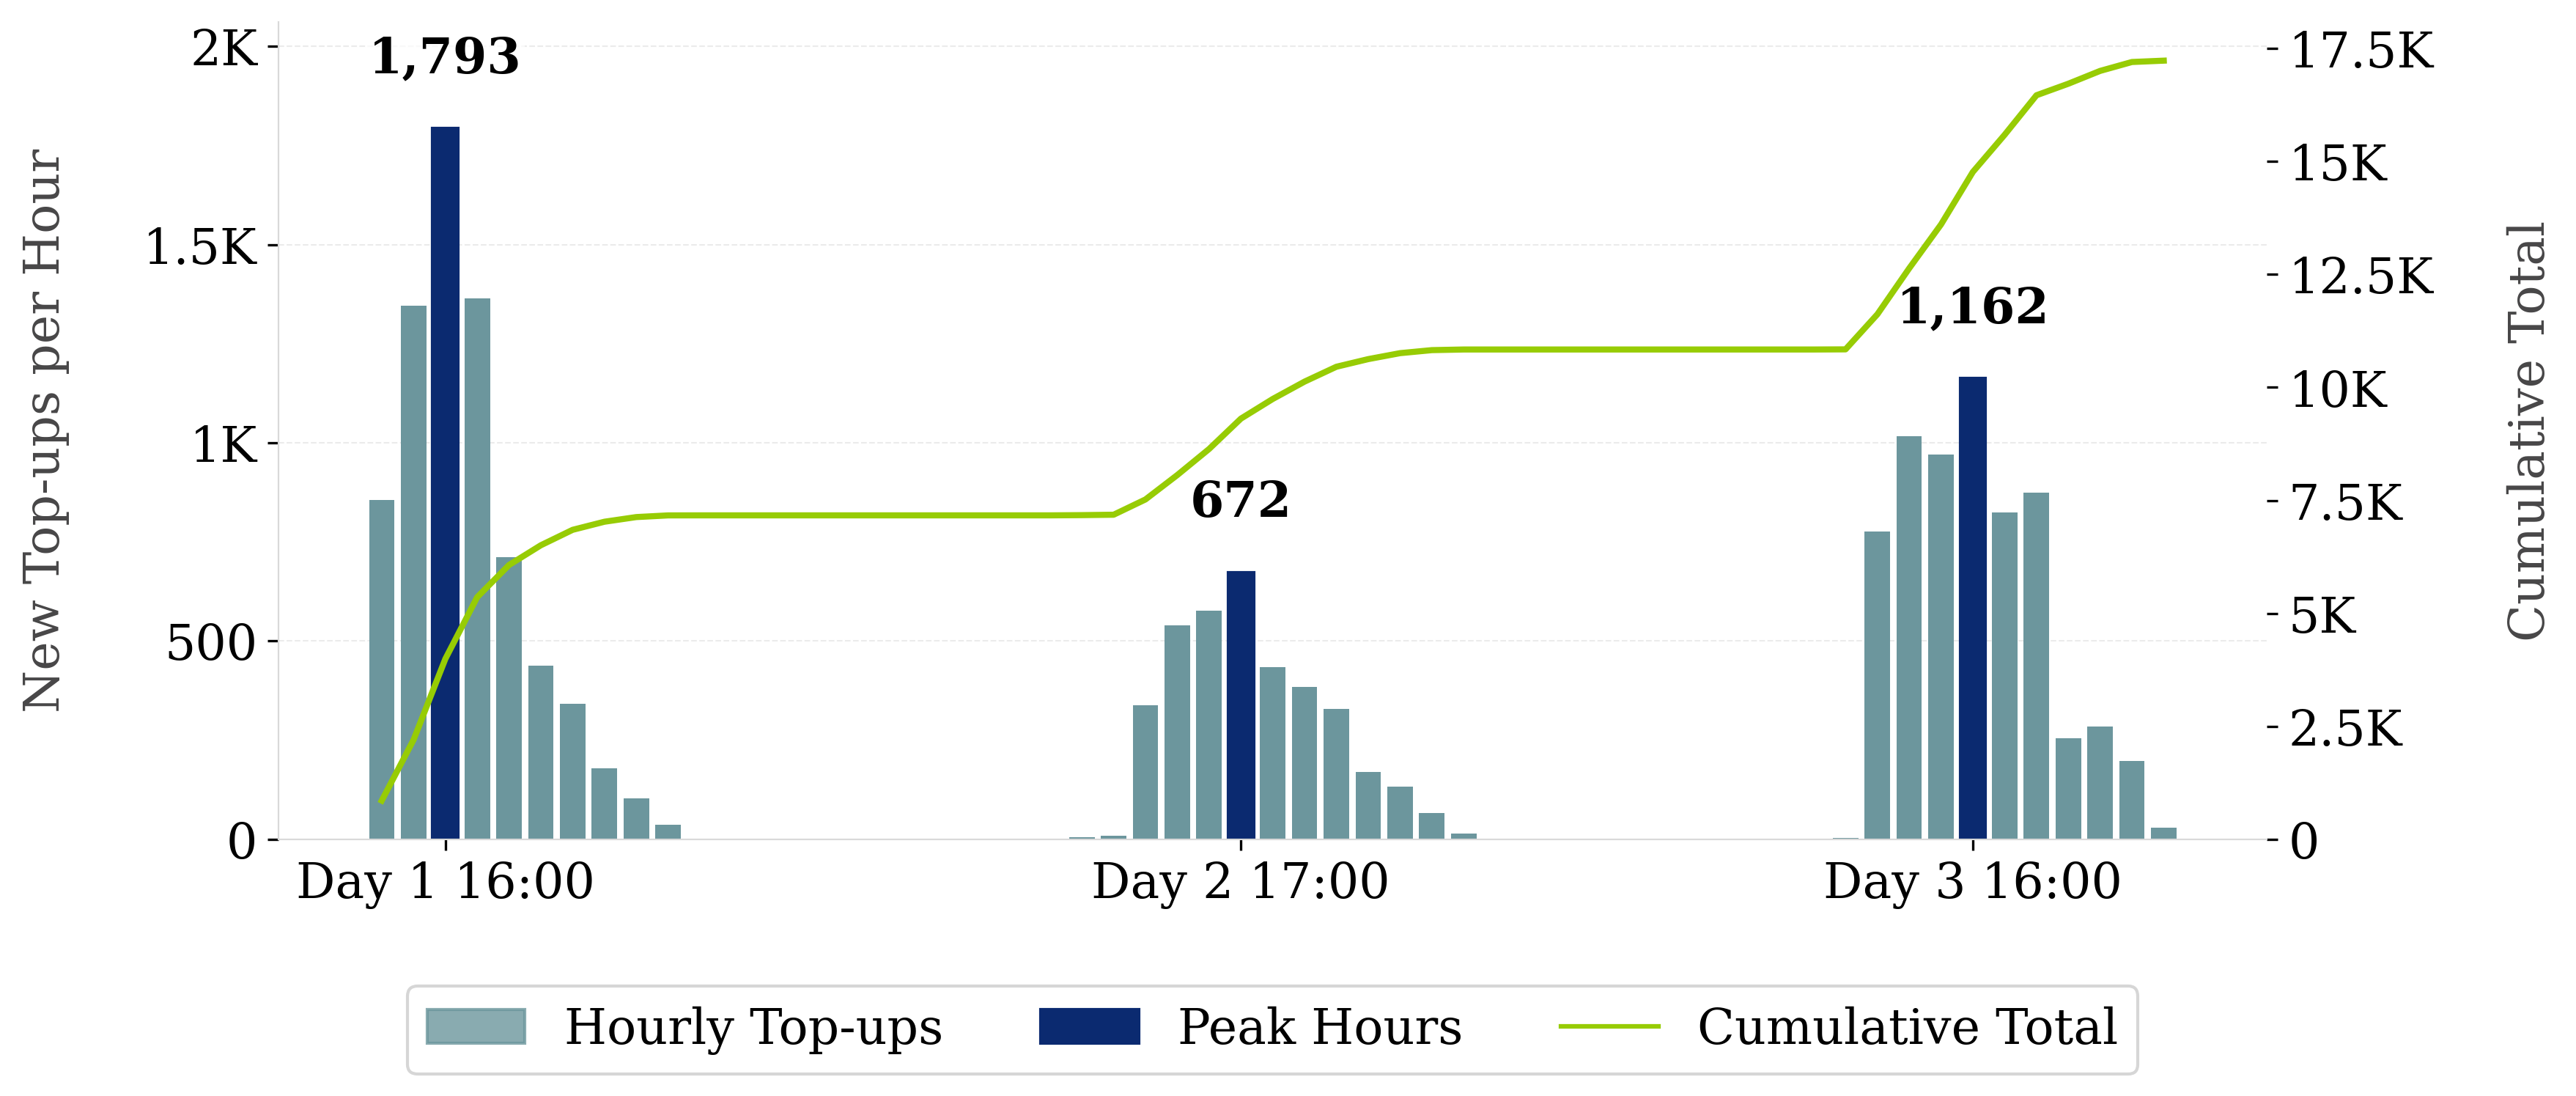
\includegraphics[width=\textwidth]{\ChartsDir/rq26-topup-patterns}
	\caption{\rqshorttext{customers-top-up-peaks} Credit Top-up Patterns During Event}
	\label{chart:topup-patterns}
	\source
\end{chart}

Each day had a similar pattern, with activity increasing in the early afternoon, peaking in the late afternoon (between 16:00 and 18:00), and gradually decreasing into the evening.
Given the festival was closed over the overnight hours (00:00--12:00), there was minimal top-up activity as expected.

\begin{keytakeaways}
	\begin{itemize}
		\item Peak top-up activity consistently occurred during late afternoon hours.
		\item Day 1 saw the highest single-hour volume with~\bfmtnum{1793}~top-ups.
		\item Day 3 showed sustained high activity with multiple hours exceeding~\bfmtnum{800}~top-ups.
		\item A consistent daily pattern of afternoon peaks and overnight declines was observed.
	\end{itemize}
\end{keytakeaways}

%%% Customer / Segmentation Analysis
%%% --------------------------------------------------------------

\subsection{Customer Segmentation}
\label{subsec:analysis-customer-segmentation}

This section analyzes the distribution of customer types and their digital service adoption patterns, providing insights into how different groups of attendees interacted with the system.

\makerqbox{customers-top-up-online}

Out of~\bfmtnum{8974}~customers who got their chips through online ticket purchases, only \bfmtnum{1630}~(\bfmtnump[1]{18.2}\%) took advantage of the advance credit top-up option.
This indicates that while many customers purchased tickets online, most preferred to top up their credit on-site.

\makerqbox{customers-distribution-types}

The festival attracted a total of~\bfmtnum{10009} attendees across different categories.
This distribution is shown in~\autoref{chart:customer-distribution} below.

\begin{chart}[H]
	\centering
	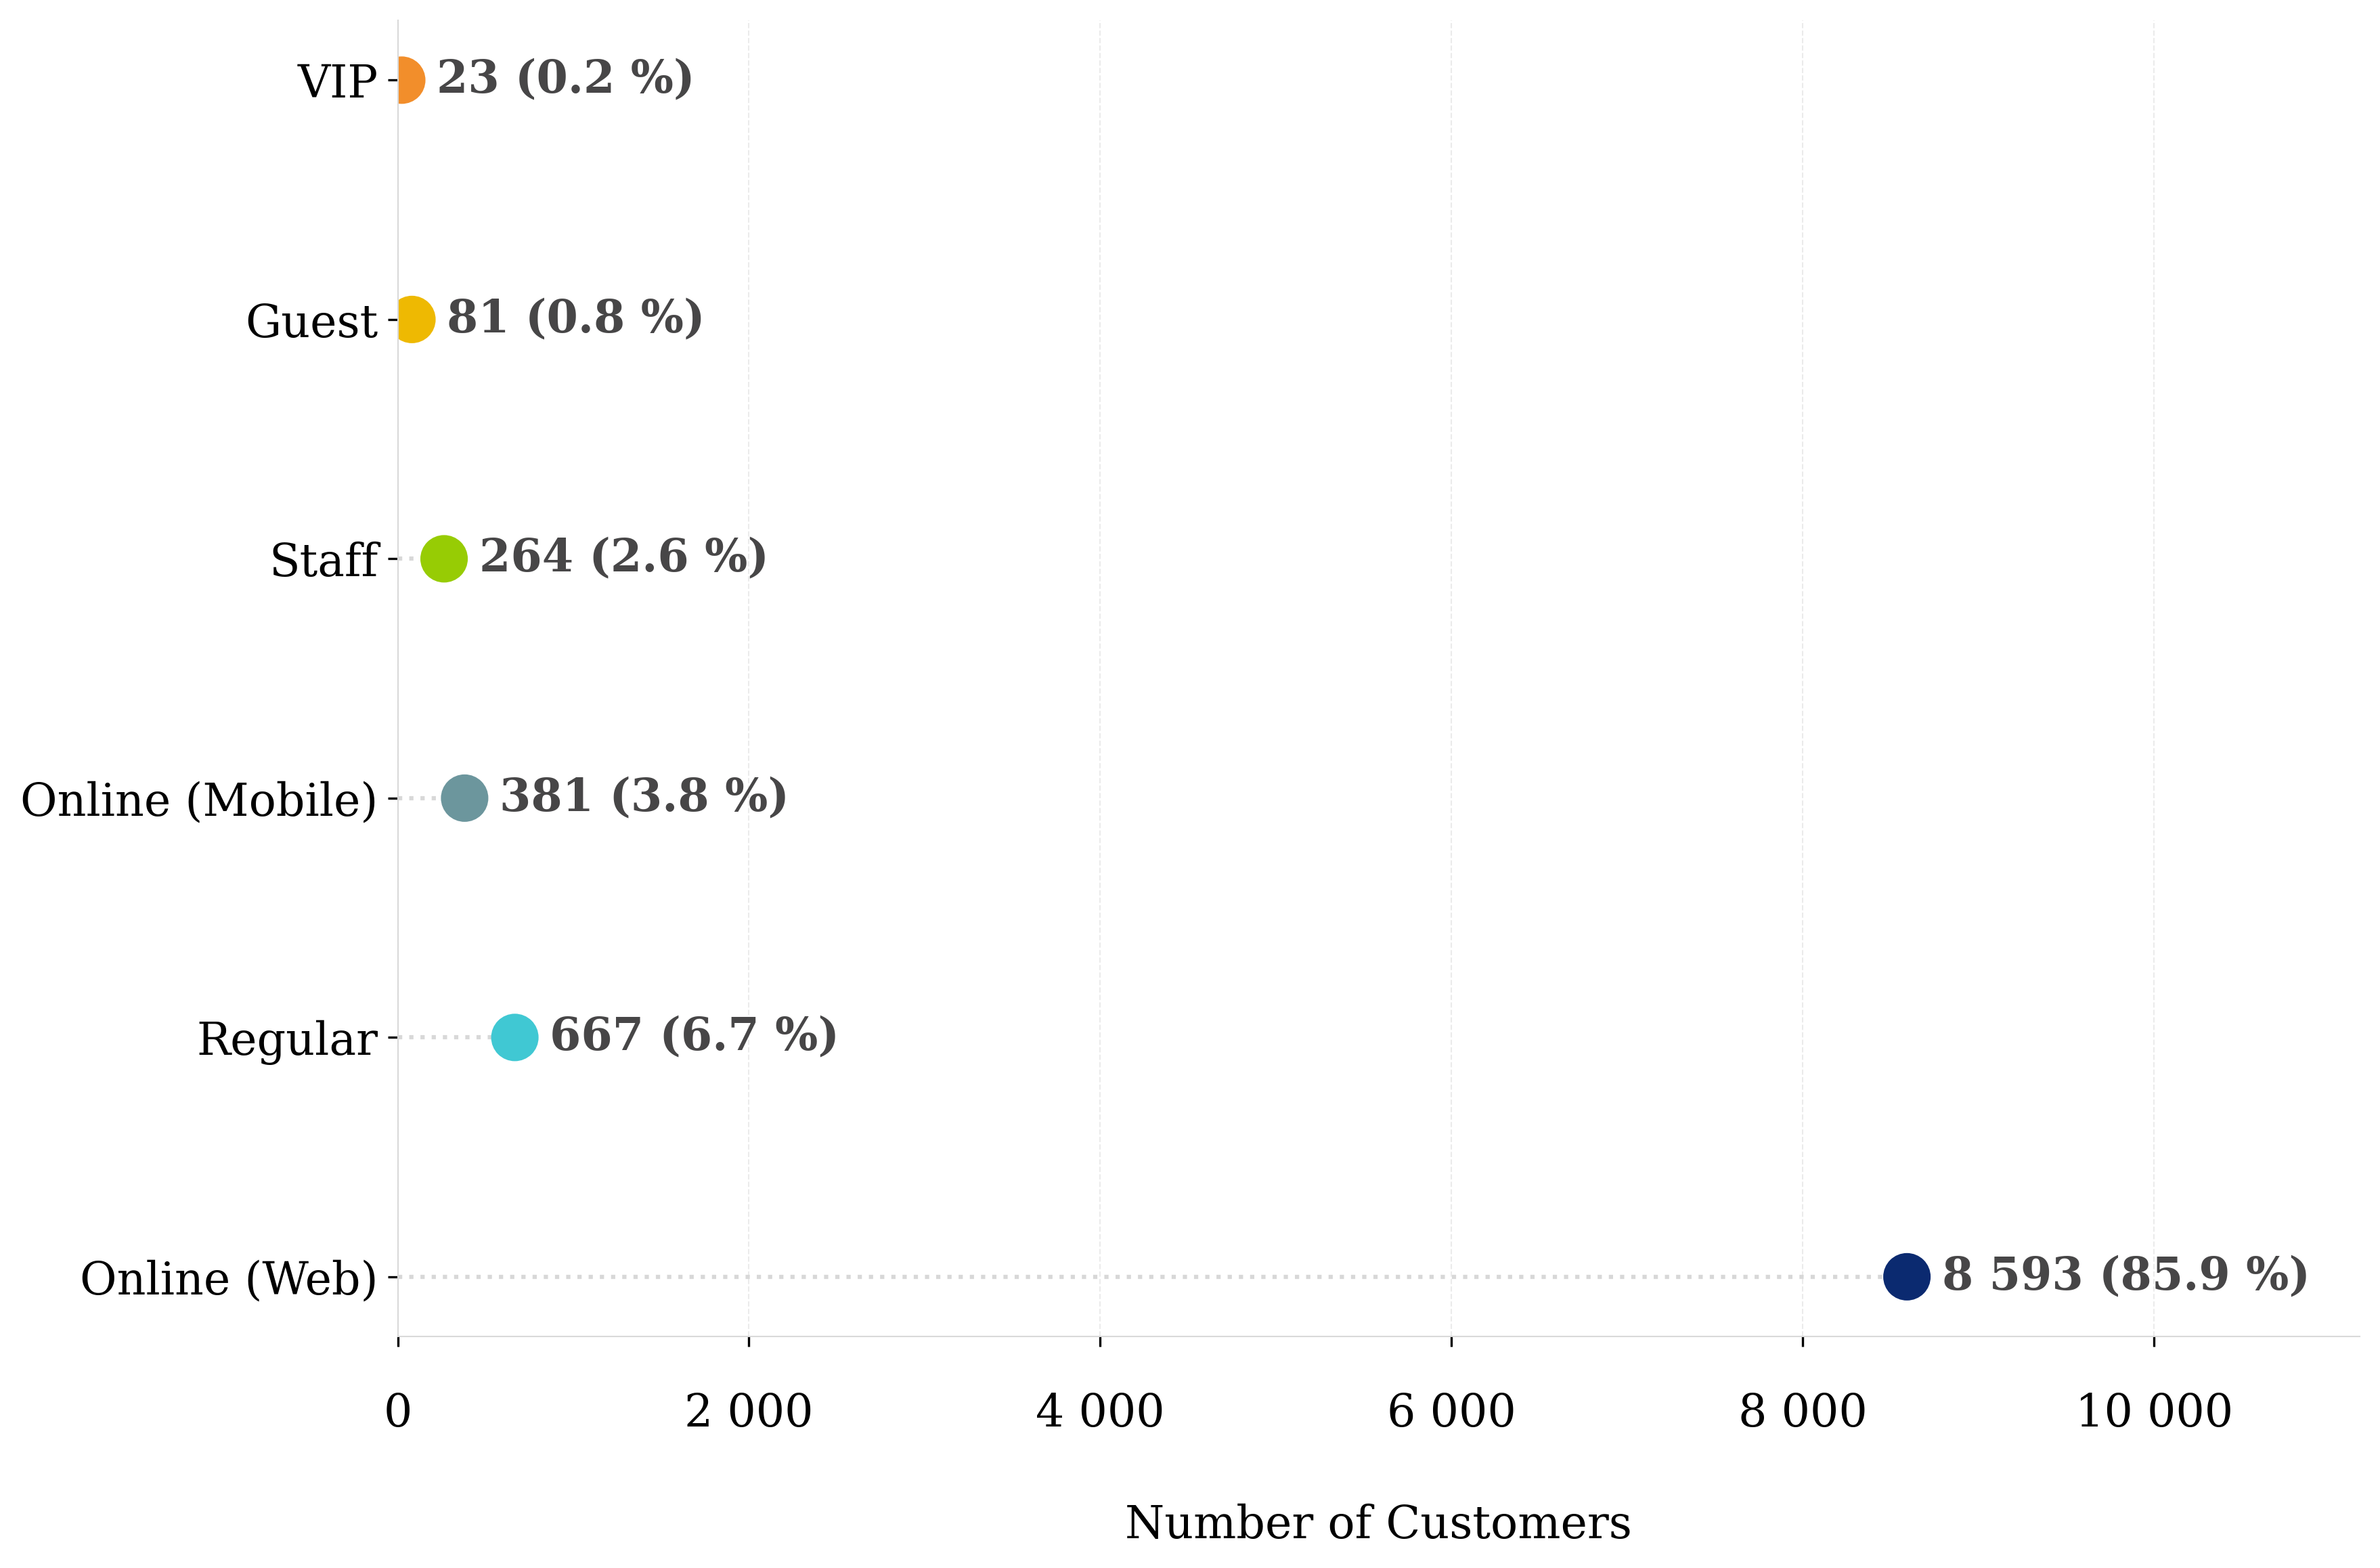
\includegraphics[width=\textwidth]{\ChartsDir/rq20-customer-distribution}
	\caption{\rqshorttext{customers-distribution-types} Customer Distribution by Type}
	\label{chart:customer-distribution}
	\source
\end{chart}

The data shows that the vast majority of attendees (\bfmtnump[1]{89.7}\%) came through online ticket purchases.
Regular customers made up~\bfmtnump[1]{6.7}\%~of attendees, while staff, guests, and VIPs collectively accounted for less than~\bfmtnum{4}\%~of the total attendance.

\makerqbox{customers-mobile-app}

The system provides several ways for customers to interact with the festival, including mobile apps and web platform.
These can be used for ticket purchases, credit top-ups, credit refunds, and other services.
This breakdown is shown in~\autoref{chart:customer-app-usage} below.

\begin{chart}[h]
	\centering
	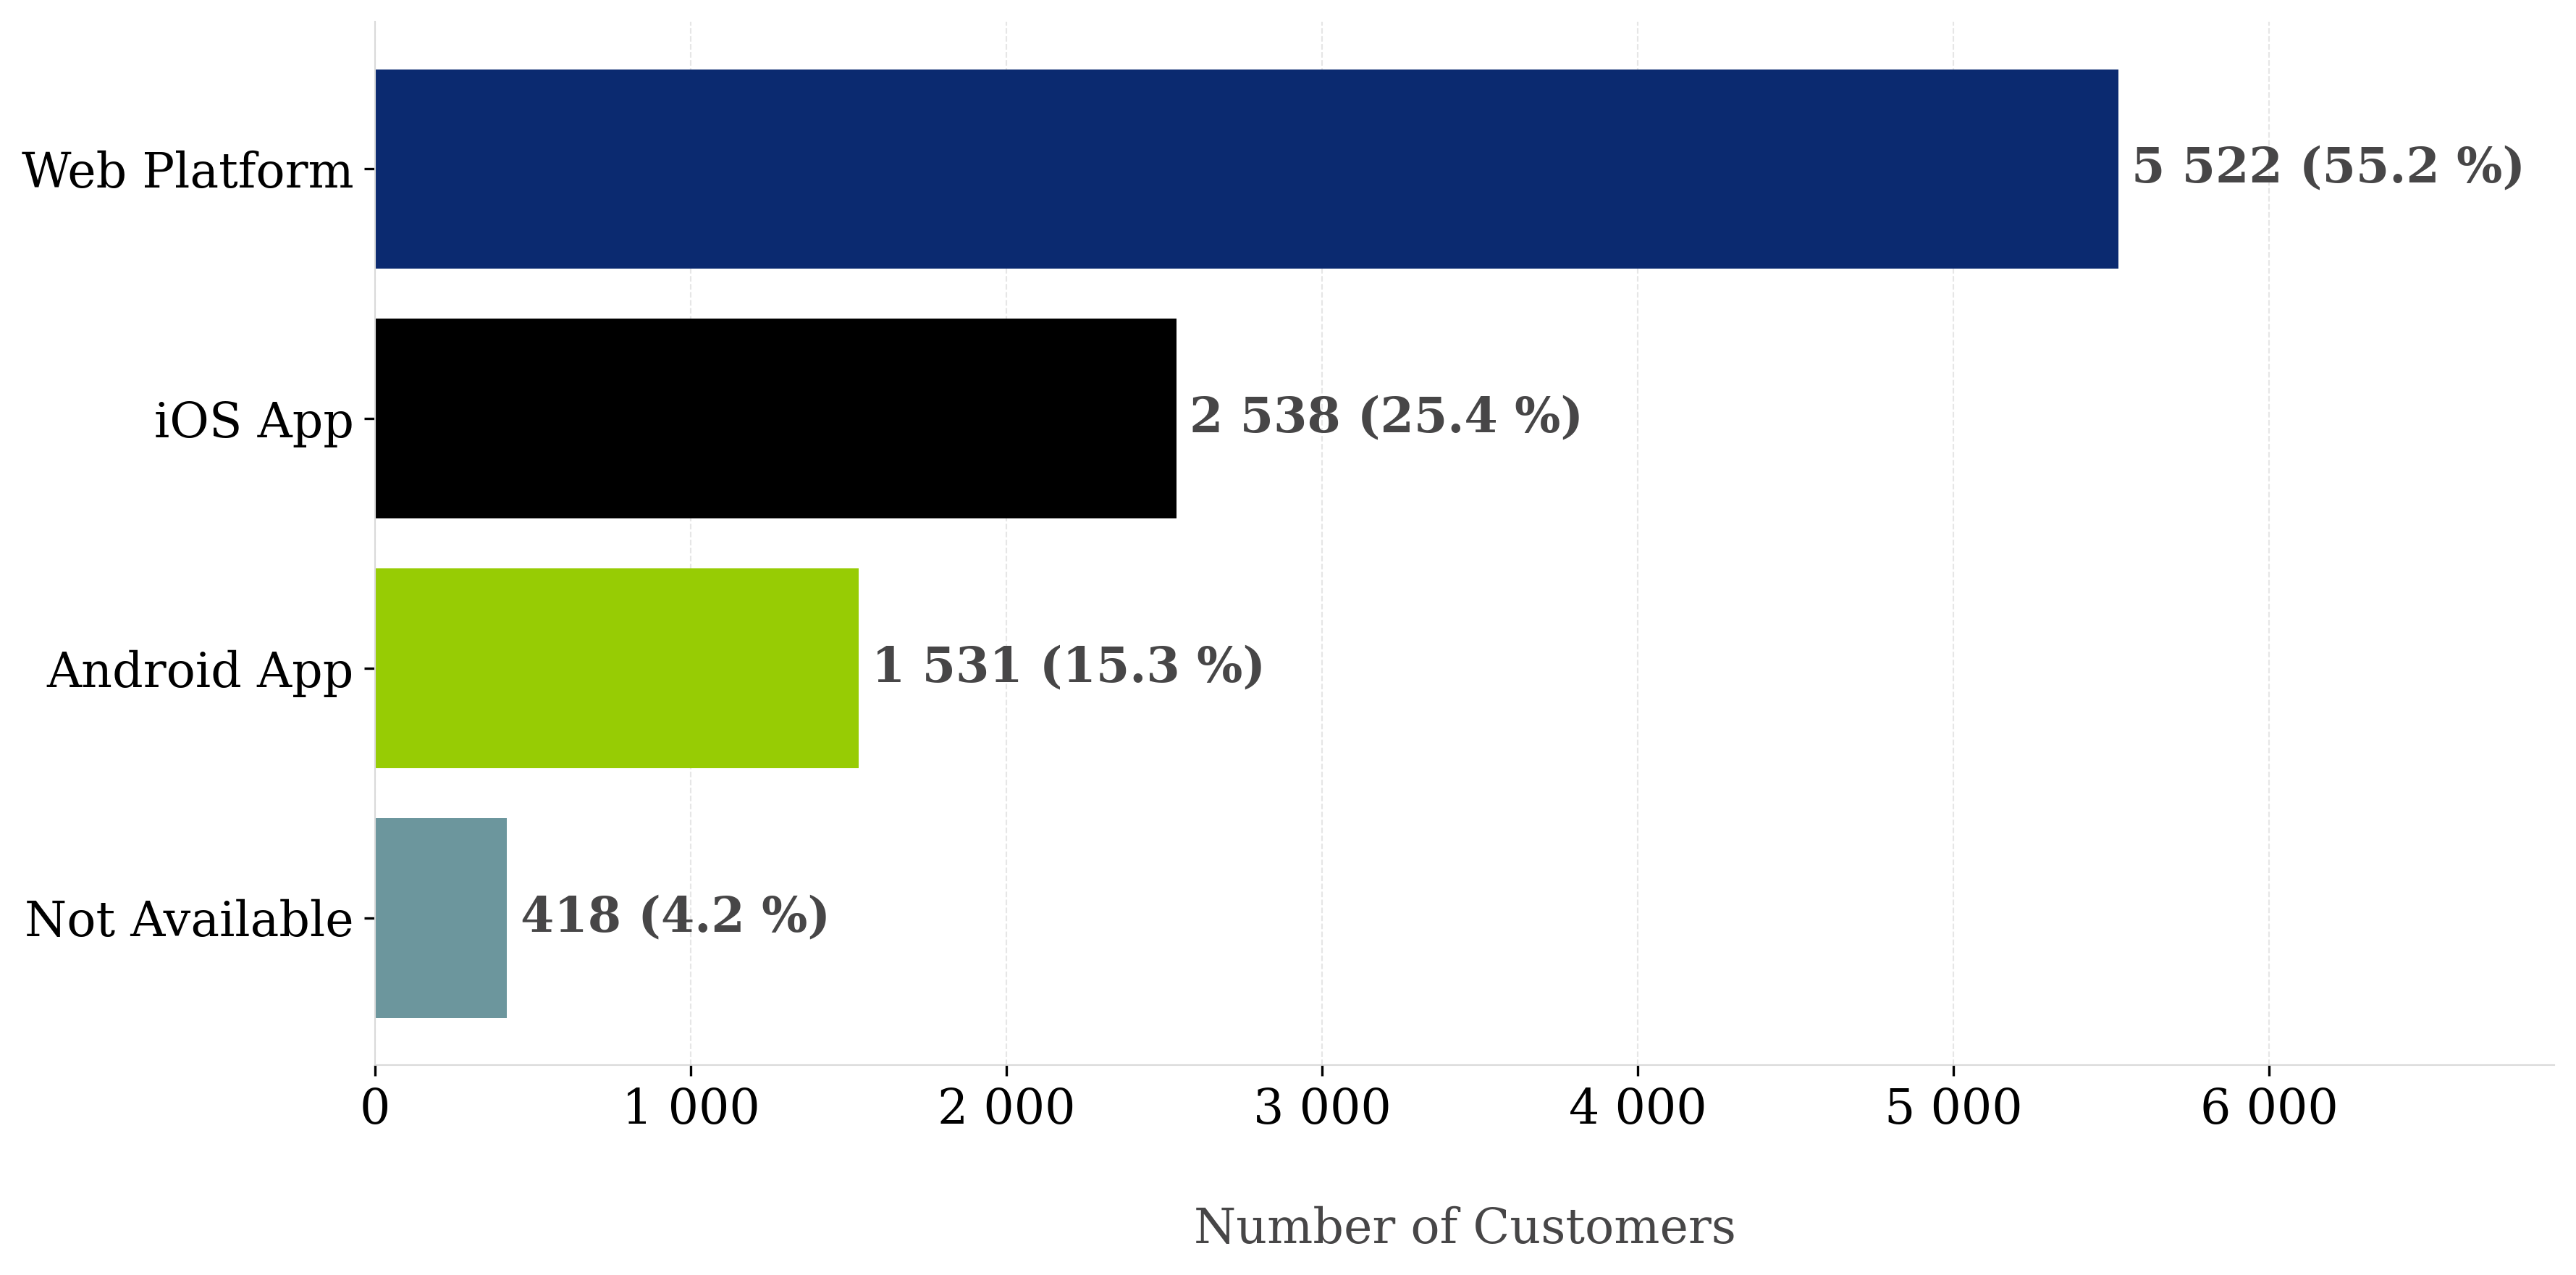
\includegraphics[width=\textwidth]{\ChartsDir/rq21-customer-app-usage}
	\caption{\rqshorttext{customers-mobile-app} Customer App Usage}
	\label{chart:customer-app-usage}
	\source
\end{chart}

The analysis reveals a significant use of mobile apps, with~\bfmtnump[2]{40.69}\%~of customers using either iOS (\bfmtnump[2]{25.36}\%) app\footnote{\url{https://apps.apple.com/cz/app/nfctron/id1595341751}}
or Android (\bfmtnump[2]{15.33}\%) app\footnote{\url{https://play.google.com/store/apps/details?id=com.nfctron.mobile}}.
The web platform remained the most used way of interaction, used by~\bfmtnump[2]{55.17}\%~of customers.
A small portion (\bfmtnump[2]{4.14}\%) of customers had no recorded platform preference whatsoever.

\begin{keytakeaways}
	\begin{itemize}
		\item Only~\bfmtnump[1]{18.2}\%~of online ticket holders preloaded their credit before the event.
		\item Online ticket purchasers dominated the attendance (\bfmtnump[2]{89.66}\%~of all customers).
		\item Mobile app usage was significant, with~\bfmtnump[2]{40.69}\%~of customers using an app.
		\item iOS app usage (\bfmtnump[2]{25.36}\%) was notably higher than Android (\bfmtnump[2]{15.33}\%).
	\end{itemize}
\end{keytakeaways}


%%% Customer / Payment Behavior Analysis
%%% --------------------------------------------------------------

\subsection{Payment Behavior Analysis}
\label{subsec:analysis-customer-payment-behavior}
This subsection focuses mainly on the payment segmentation and behavior of festival attendees.

By segmenting the customers based on their payment data,
such as their card-issuing banks
\footnote{Card Issuing bank is the bank responsible for issuing payment cards to customers; Issuers manage cardholder accounts, authorize transactions, and handle billing\cite{jc_what_are_card_schemes_and_how_do_they_work}} and used
payment card schemes\footnote{Card Scheme, such as Mastercard or Visa, are a payment network provider who processes card payments globally\cite{jc_what_are_card_schemes_and_how_do_they_work}}, the analysis should find interesting
patterns and answer the defined research questions.

\makerqbox{customers-bank-cards}

The analysis of bank refunds reveals the distribution among Czech banking institutions shown in~\autoref{chart:bank-refunds} below.

\begin{chart}[h]
	\centering
	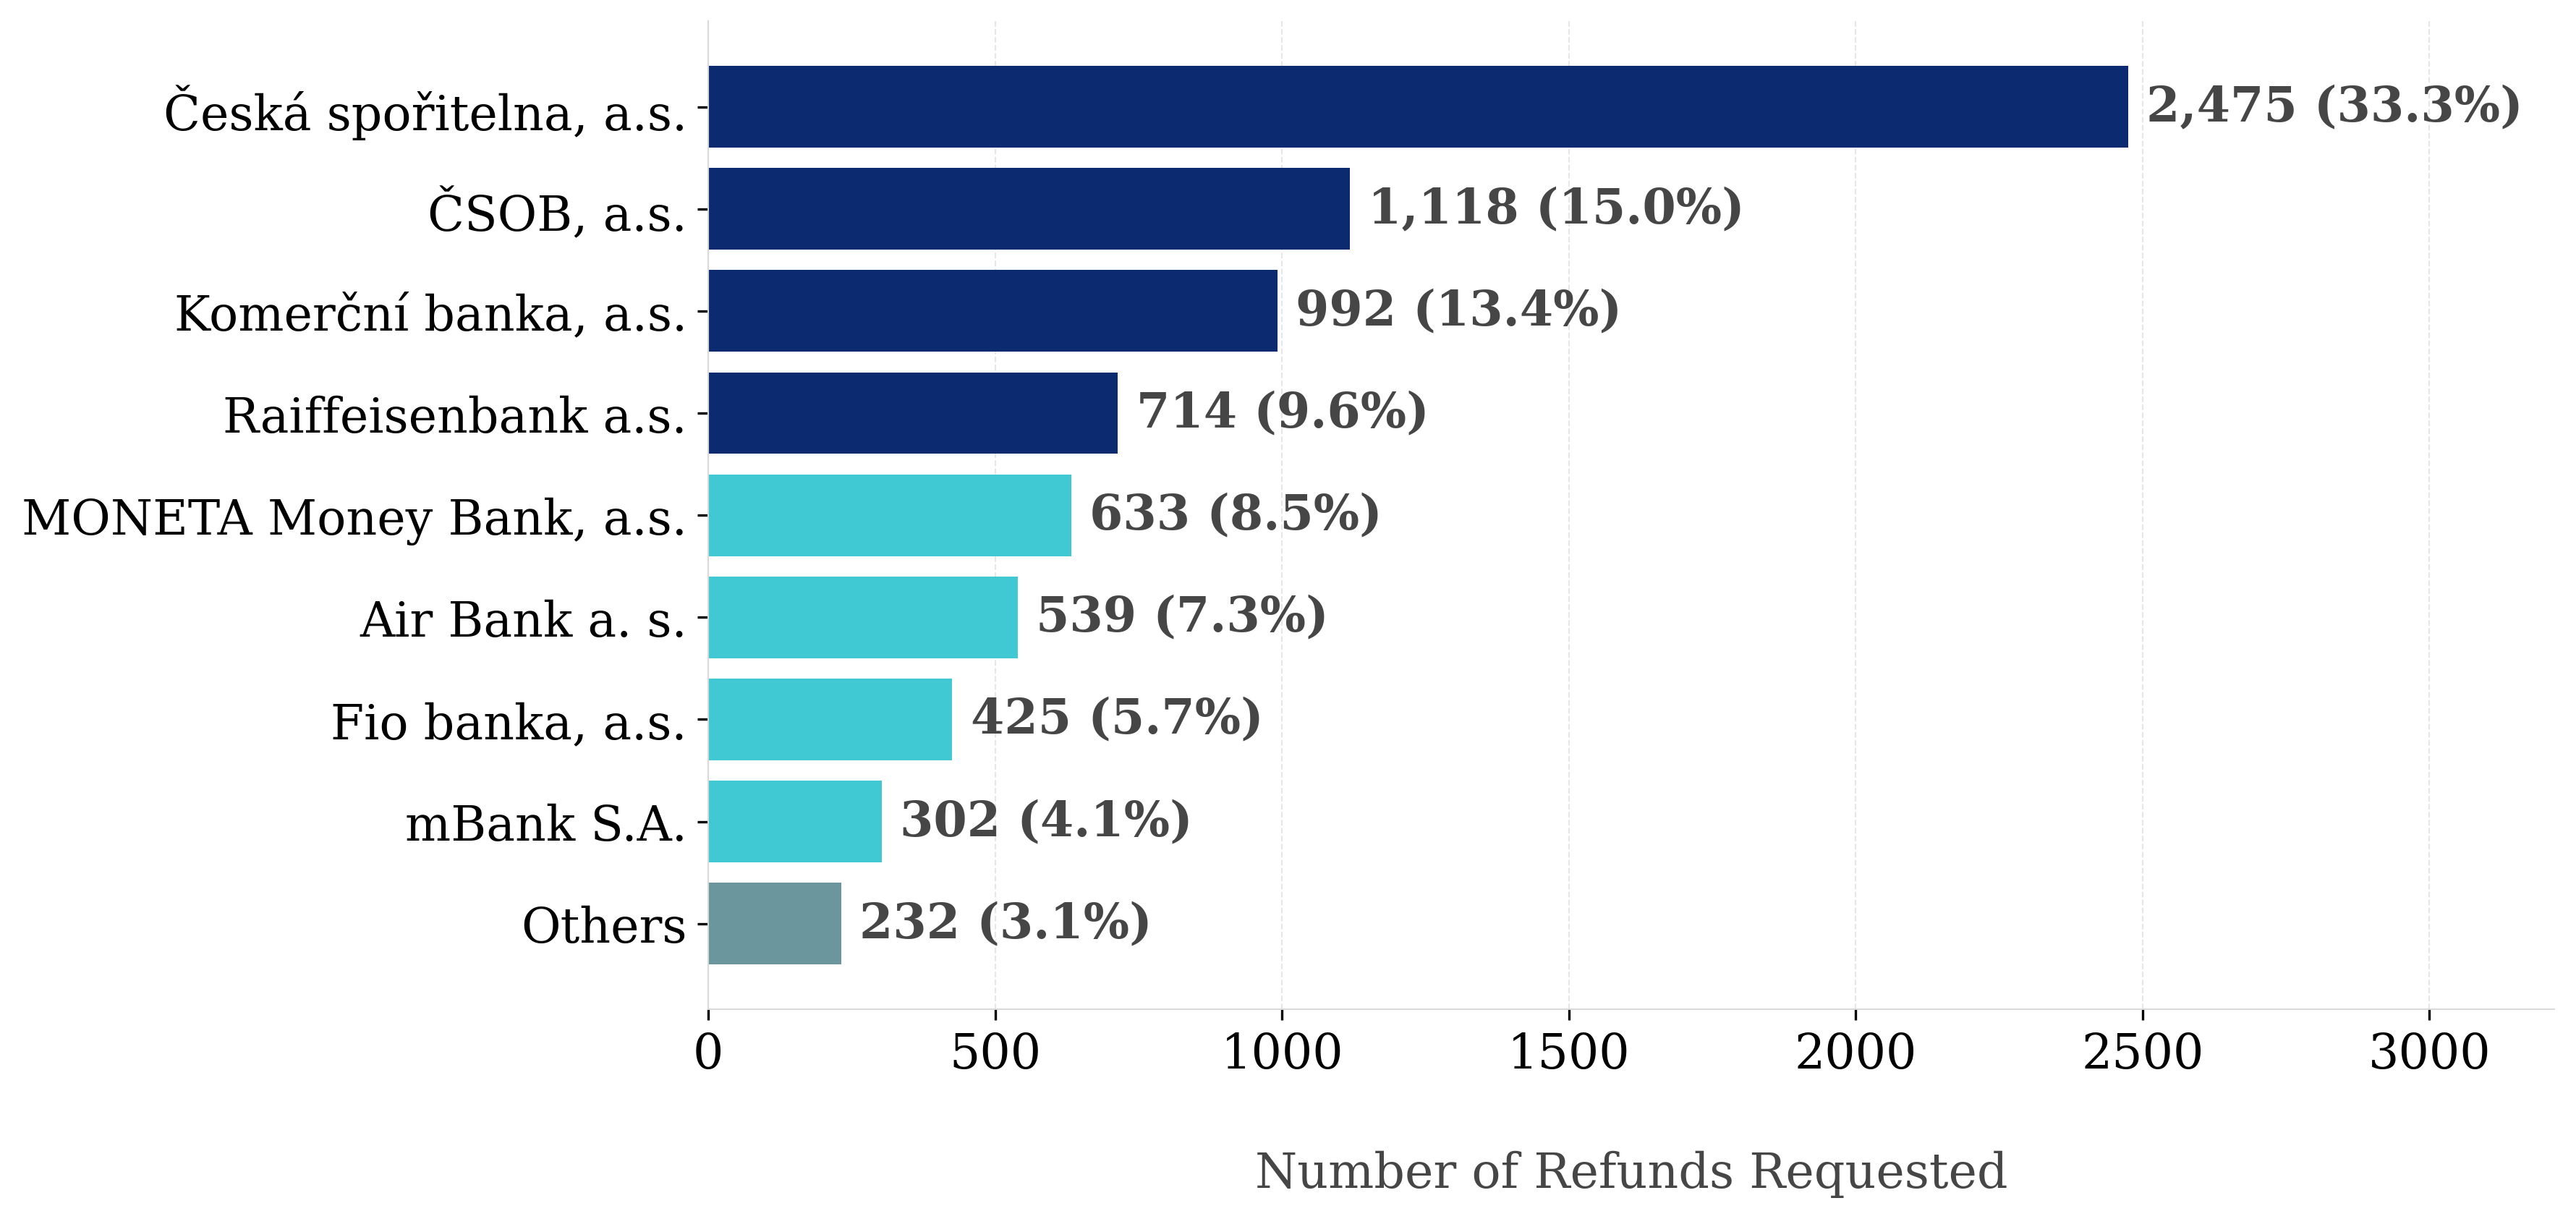
\includegraphics[width=\textwidth]{\ChartsDir/rq22-bank-refunds}
	\caption{\rqshorttext{customers-bank-cards} Bank Refunds Distribution}
	\label{chart:bank-refunds}
	\source
\end{chart}

Out of the~\bfmtnum{7430}~online credit refunds that were requested, the data shows that \textbf{Česká spořitelna} was the leading bank, accounting for~\bfmtnump[1]{33.3}\%~of all refunds.
Followed by \textbf{ČSOB} and \textbf{Komerční banka} with~\bfmtnump[1]{15}\%~and~\bfmtnump[1]{13.4}\%~share respectively.

\makerqbox{customers-card-schemes}

\begin{chart}[h]
	\centering
	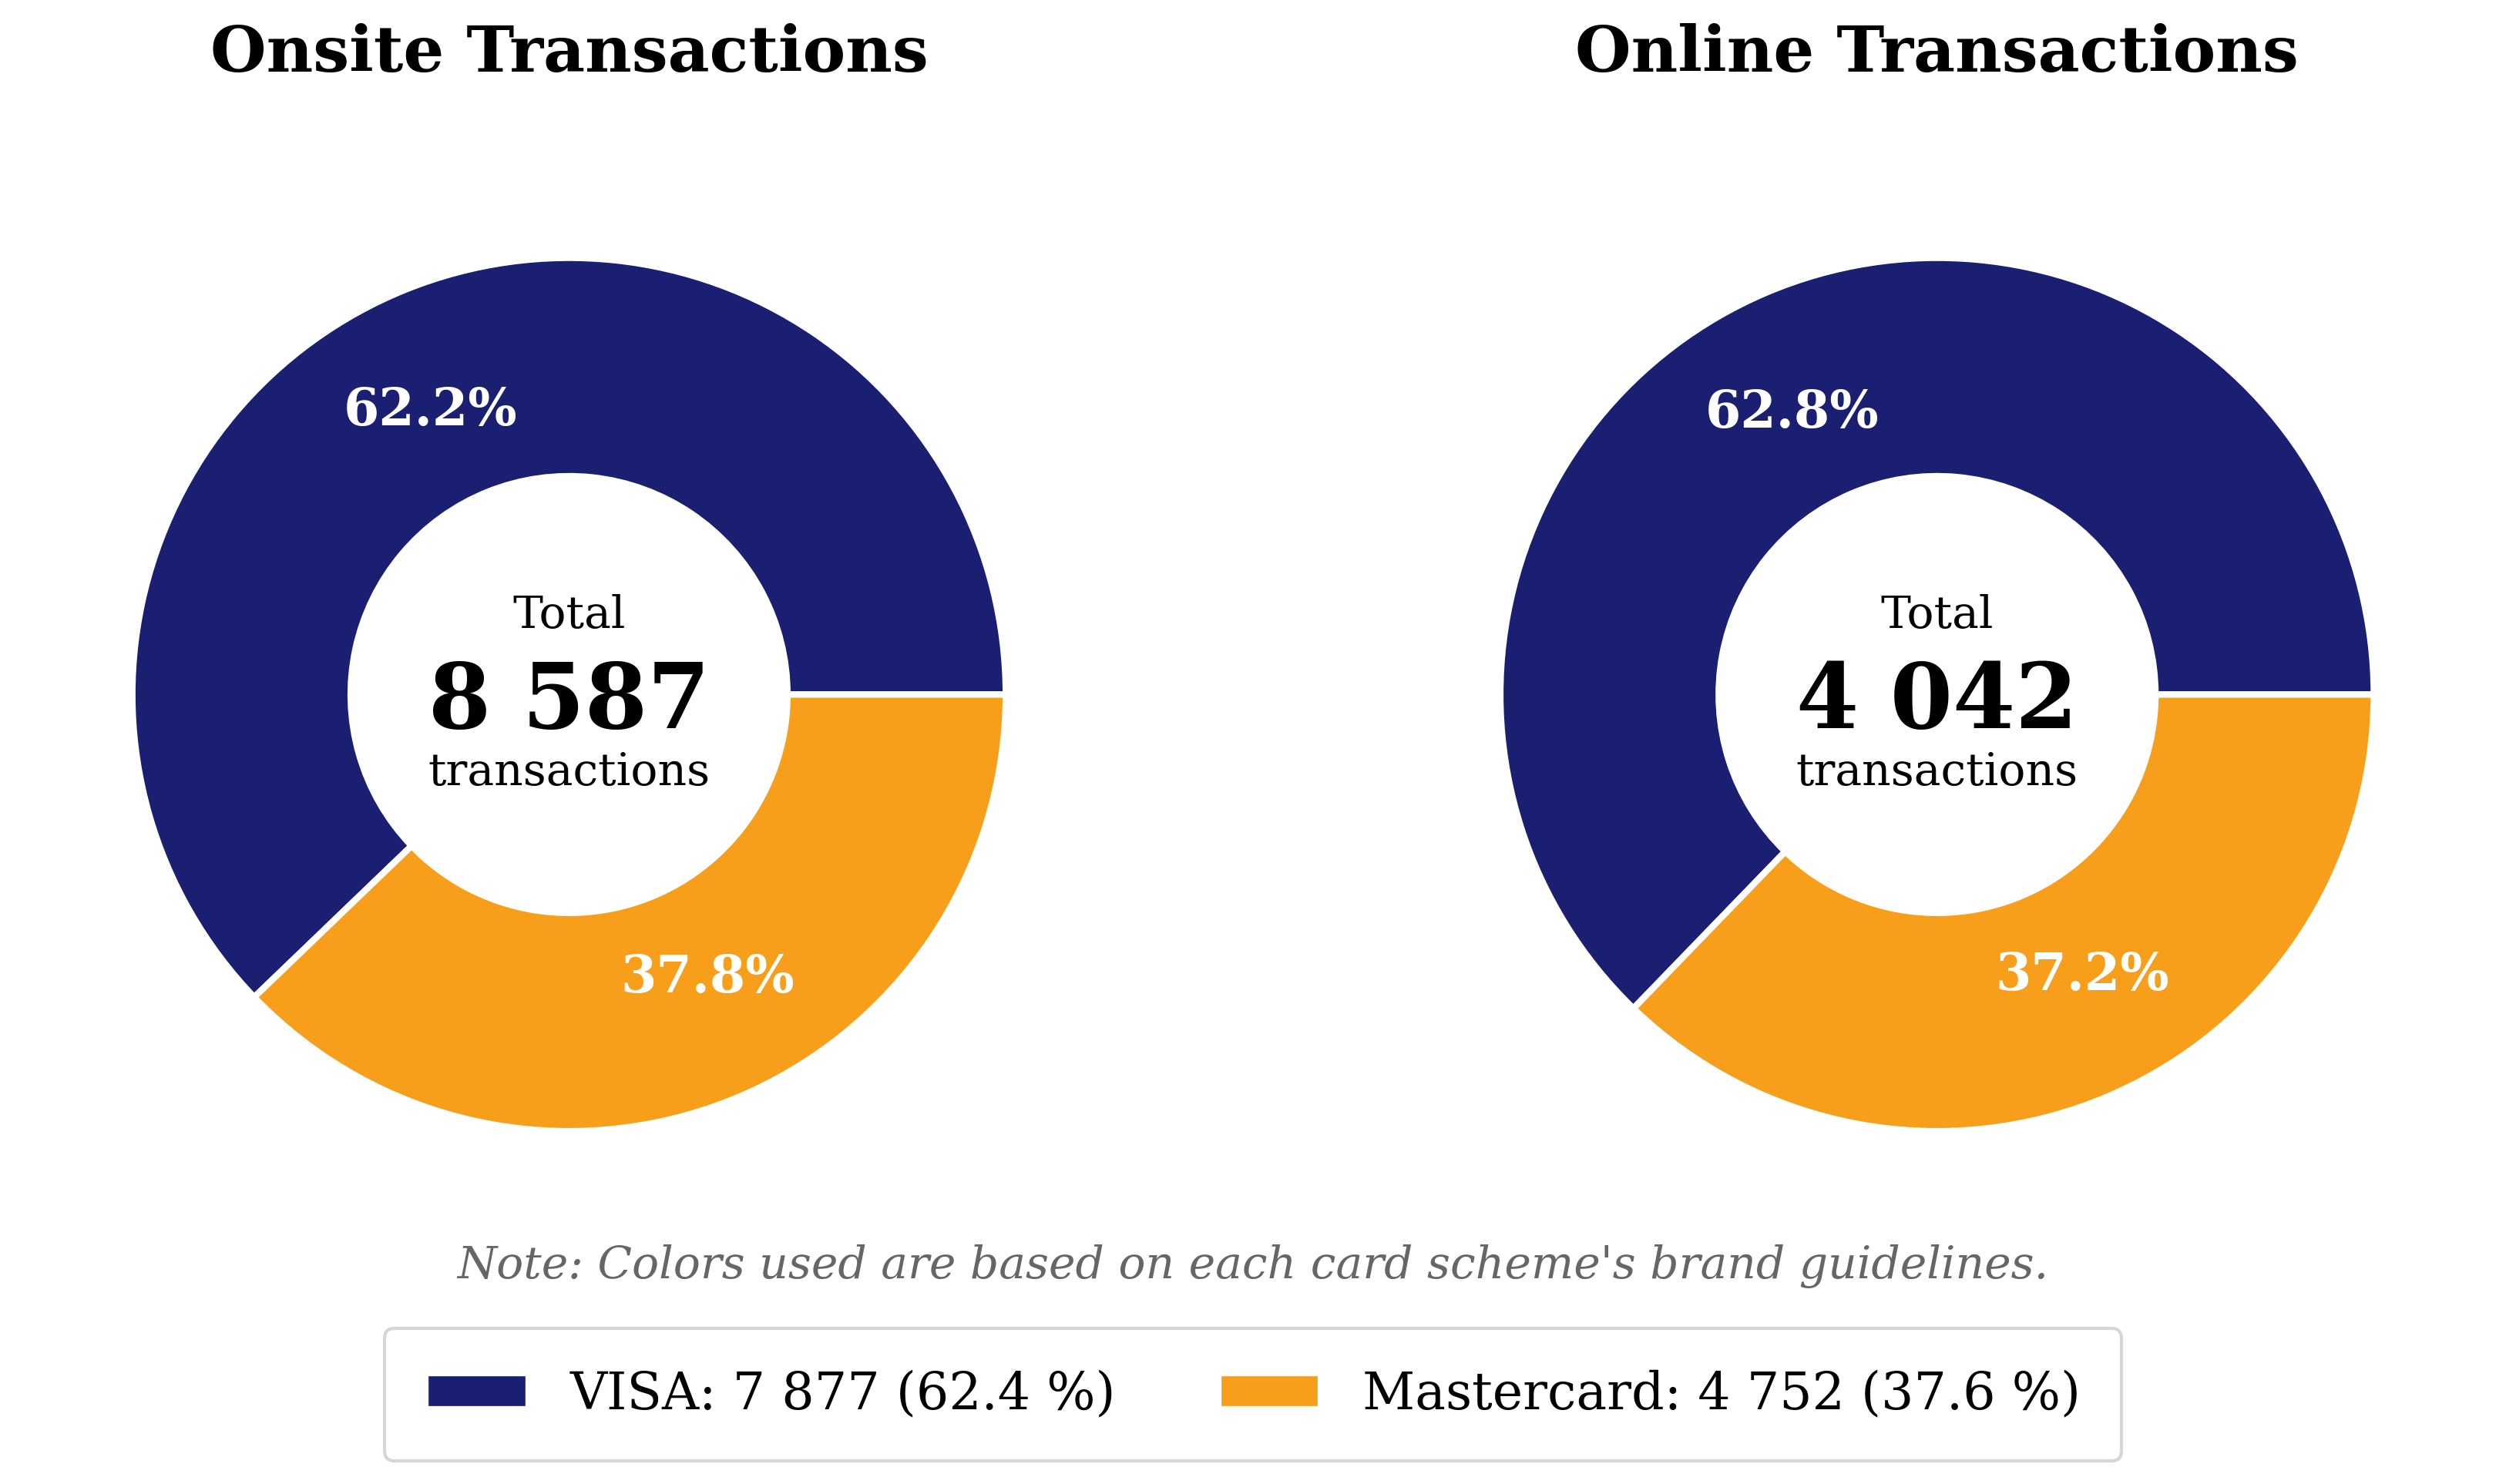
\includegraphics[width=\textwidth]{\ChartsDir/rq23-card-schemes}
	\caption{\rqshorttext{customers-card-schemes} Card Schemes Distribution}
	\label{chart:card-schemes}
	\source
\end{chart}

Out of total \bfmtnum{12626}~card transactions done both online (online ticket purchases, credit top-ups in advance) and onsite (onsite top-ups at festival, onsite physical ticket purchases), only two card schemes were identified:
\begin{itemize}
	\item \textbf{VISA} cards were used in~\bfmtnump[1]{62.4}\%~of transactions, making them the dominant card scheme.
	\item \textbf{Mastercard} cards followed at~\bfmtnump[1]{37.6}\%~of transactions.
\end{itemize}

This distribution rather nicely follows the Czech market trend, where VISA is the most used card scheme with \bfmtnum{65}\%~market share and Mastercard with \bfmtnum{35}\%~market share\cite{spbk_czech_profil_karty}.

\pagebreak[4]

\makerqbox{customers-top-up-frequency}

Analyzing onsite top-up frequency behavior at the festival reveals the distribution of top-up counts among customers, as shown in~\autoref{chart:top-up-behavior} below.

\begin{chart}[h]
	\centering
	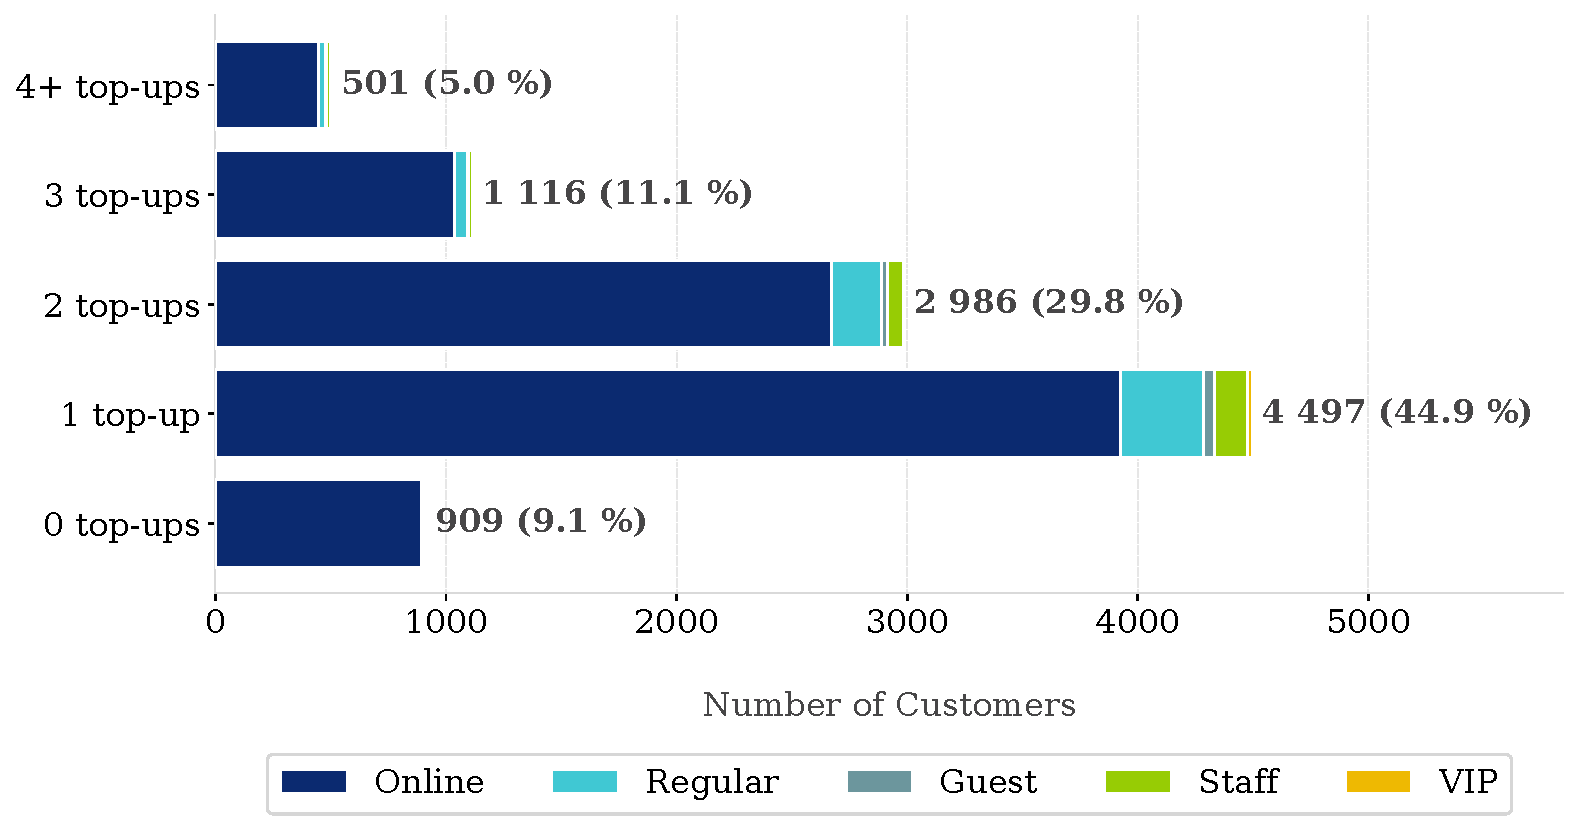
\includegraphics[width=\textwidth]{\ChartsDir/rq27-topup-frequency}
	\caption{\rqshorttext{customers-top-up-frequency} Top-up Behavior Analysis}
	\label{chart:top-up-behavior}
	\source
\end{chart}

The analysis of top-up behavior reveals that most customers (\bfmtnump[1]{44.9}\%) topped up only once during the festival.
A significant portion (\bfmtnump[1]{29.8}\%) topped up twice, while only a small fraction of customers (\bfmtnump[0]{5}\%) topped up more than three times.

An interesting finding is that around~\bfmtnump[0]{9}\%~of customers did not top up at onsite at all.
This meant for Online customers that they preloaded their credit before the event and did not need nor required to top up during the festival.
For other on-site registered customers, it meant they did not use their chip bracelet for payments at all, but only as an entry ticket or for access control purposes.

\begin{keytakeaways}
	\begin{itemize}
		\item The most common bank for refunds was \textbf{Česká spořitelna} (\bfmtnump[1]{33.3}\%).
		\item \textbf{VISA} cards were more used (\bfmtnum{62}\%) compared to \textbf{Mastercard} (\bfmtnum{37}\%).
		\item The majority of customers (\bfmtnump[1]{74.7}\%) topped up their credit 1 or 2 times during the event.
		\item Very few customers (\bfmtnum{5}\%) needed four or more top-ups.
	\end{itemize}
\end{keytakeaways}

%%% Customer / Purchase Pattern Analysis
%%% --------------------------------------------------------------

\subsection{Purchase Pattern Analysis}
\label{subsec:analysis-customer-purchase-pattern}

This section examines customer purchase behaviors throughout the festival, focusing on beverage preferences across different times of day and common product combinations.

%%% Customer / Purchase Pattern Analysis / Beverage Preferences

\subsubsection{Beverage Preferences Throughout the Day}
\label{subsubsec:analysis-beverage-preferences}

\makerqbox{customers-drink-preferences}

To analyze beverage preferences throughout the day, sales data was aggregated by hour and beverage category.
A~\autoref{chart:beverage-preferences}~shows the distribution of alcoholic and non-alcoholic beverage sales over the course of the day.

\begin{chart}[h]
	\centering
	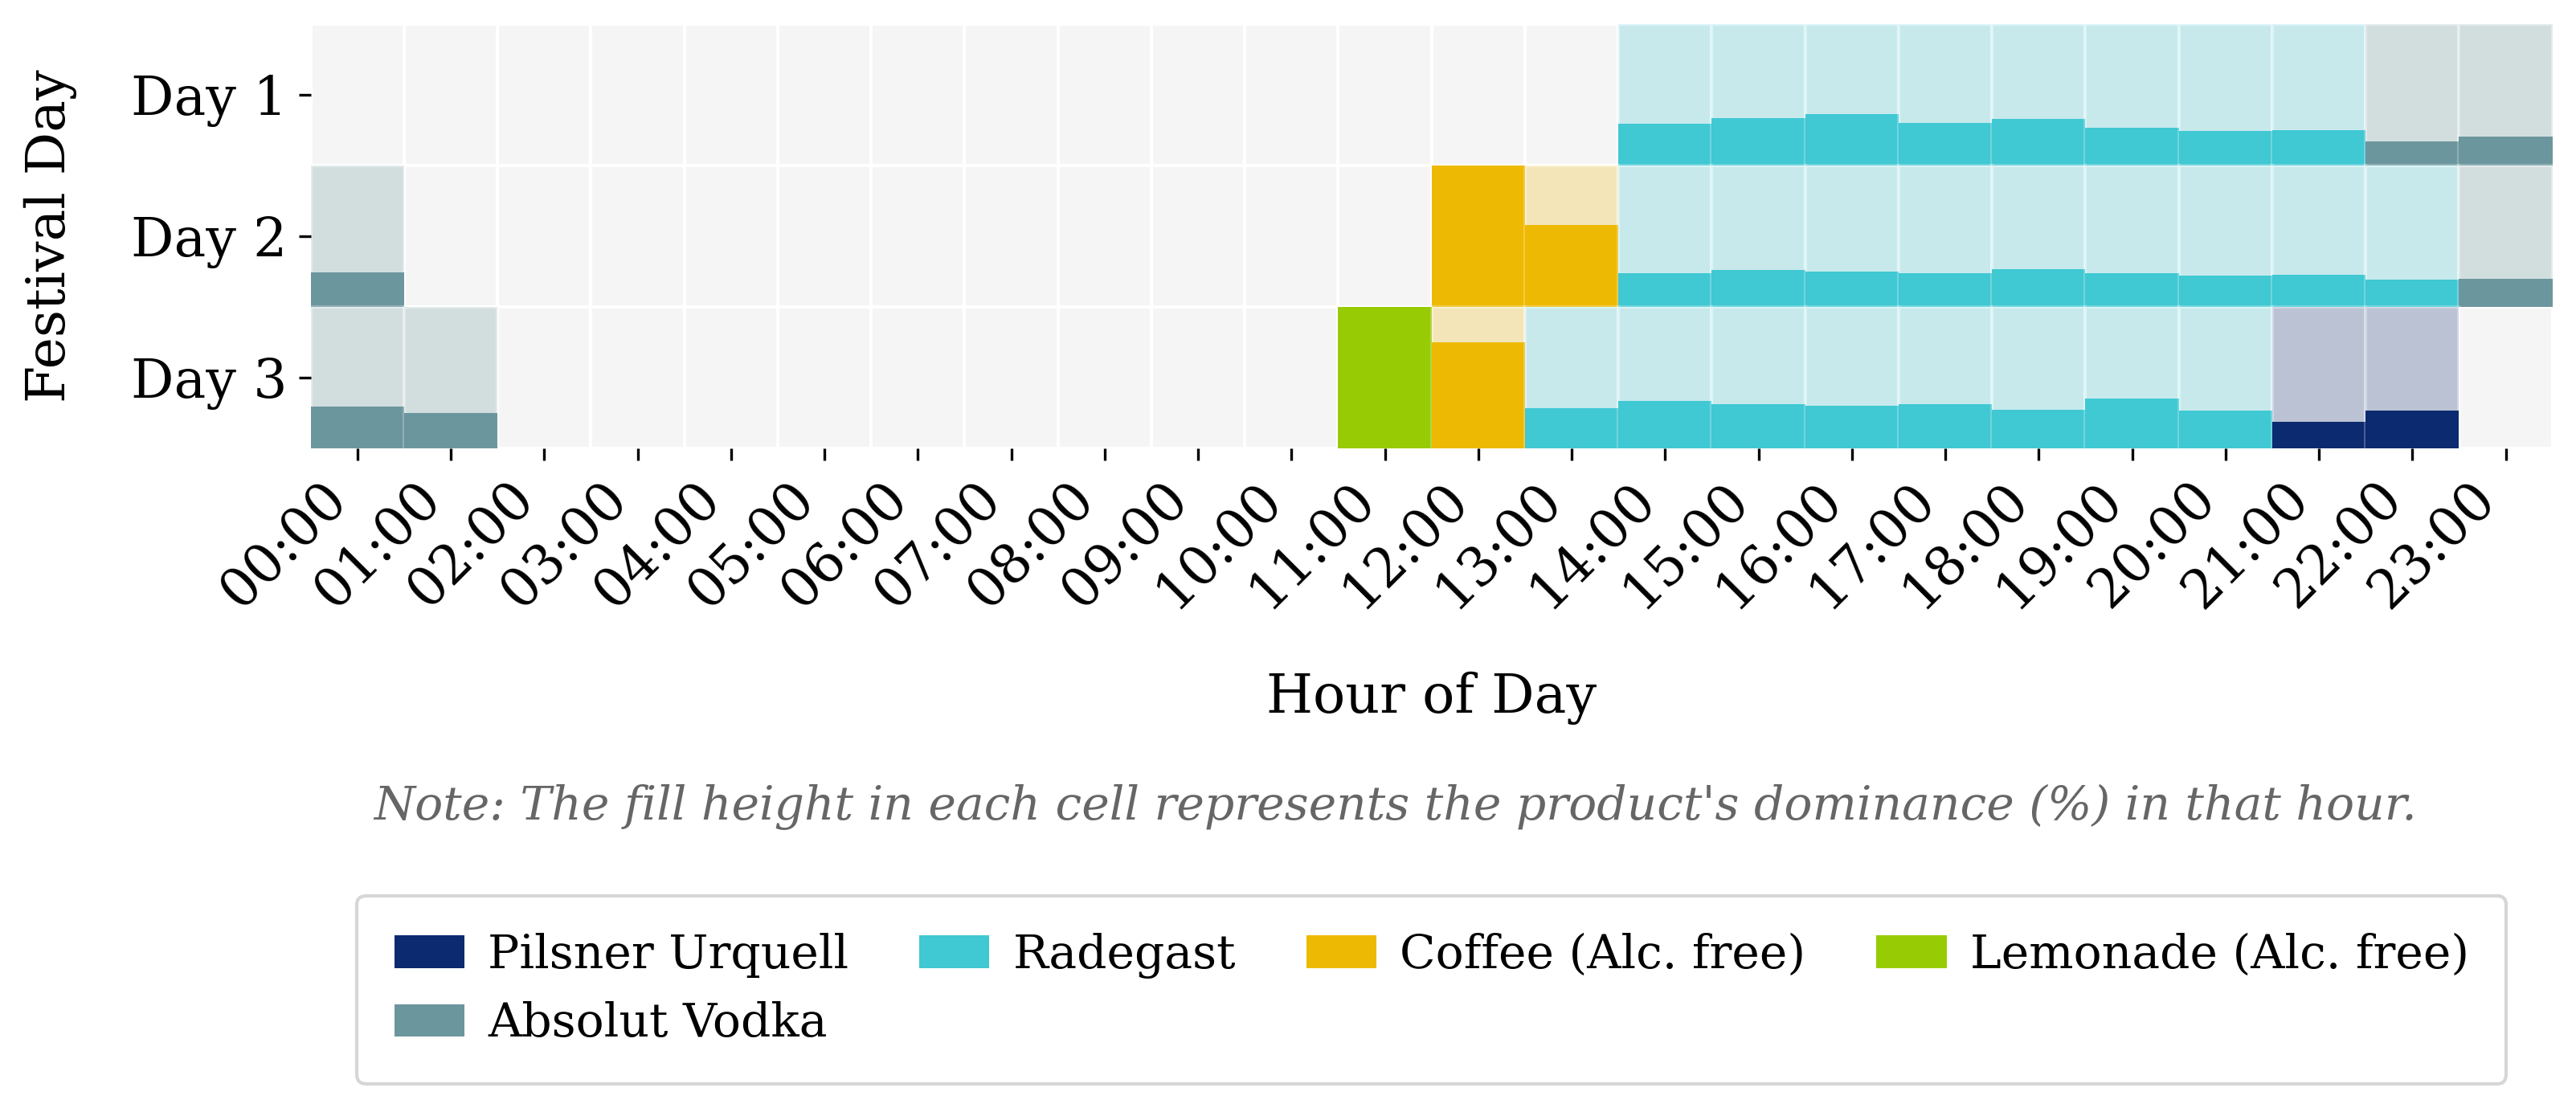
\includegraphics[width=\textwidth]{\ChartsDir/rq28-beverage-preferences}
	\caption{\rqshorttext{customers-drink-preferences} Beverage Preferences Throughout the Day}
	\label{chart:beverage-preferences}
	\source
\end{chart}

These results reveal that non-alcoholic beverages, such as Coffee and Lemonades, were most popular around noon.
Afternoon hours saw a shift towards light alcoholic beverages, with beer sales peaking in the late afternoon and early evening.

The beer preferences also show and confirm previous findings that Radegast was the most popular beer brand, with Pilsner Urquell following closely behind, especially at the end of the festival on Day 3.

Late evening hours saw a shift towards spirits and shots, with Absolut Vodka emerging as the most popular choice.

Hours without any preferences indicate that no sales were recorded during those times, or that the sales were too low (\(\leq 10\)~products sold in an hour) to be considered significant.

This showed no sales data throughout the night and early morning, which is expected.
However, one interesting observation is the lack of sales at the end of the festival on Day 3 after 22:00, which would indicate the festival's closing time.

\begin{infobox}{Why would a festival close at 22:00 on a Saturday?}
	The festival ended prematurely on Day 3 due to an unexpected change in weather, which later resulted in evacuation of the festival grounds.
\end{infobox}

This information was not possible to extract from the data alone, but it was a known fact from the festival organizer.

\begin{keytakeaways}
	\begin{itemize}
		\item Non-alcoholic beverages were most popular around noon.
		\item Beer sales peaked in the late afternoon and early evening.
		\item Radegast was the most popular beer brand throughout the festival.
		\item Absolut Vodka was the most popular spirit in the late evening.
		\item The festival ended prematurely on Day 3 due to an unexpected change in weather.
	\end{itemize}
\end{keytakeaways}

%%% Customer / Purchase Pattern Analysis / Common Product Combinations

\subsubsection{Common Product Combinations}
\label{subsubsec:analysis-common-combinations}

\makerqbox{customers-common-combinations}

Identifying frequently purchased product combinations can provide valuable insights into customer preferences and behavior.
Two analyses were performed: one with returnable cups and one without, as the high frequency of cup purchases can obscure other meaningful patterns.

The initial results are shown in~\autoref{chart:common-combos-with-cups}~below and as expected, returnable cups appear prominently in the most popular combinations as it was necessary to purchase them for drinks.

\begin{chart}[h]
	\centering
	\small
	% table
	% @formatter:off
	\begin{tabularx}{\textwidth}{
		|>{\columncolor{unicorn_blue!5}}X
		|>{\columncolor{unicorn_blue!5}}X
		|>{\columncolor{unicorn_blue!5}}r
		|>{\columncolor{unicorn_blue!5}}r|
	}
		\hline
		\rowcolor{unicorn_blue}
		\textbf{\color{white}Product A}
		& \textbf{\color{white}Product B}
		& \textbf{\color{white}Count}
		& \textbf{\color{white}\%~of~total }
		\\
		\hline
		\csvreader[
		head to column names,
		late after line={\\\hline},
		filter={\thecsvinputline<9}
		]{\DataDir/rq29-product-combos-with-returnable.csv}{
			product1=\producta,
			product2=\productb,
			combination_count=\combos,
			percentage_of_all_transactions=\percentage
		}{
			\producta
			& \productb
			& \num[group-separator={,}]{\combos}
			& \num[round-precision=2]{\percentage}\%
		}
		\hline
	\end{tabularx}
	% @formatter:on
	% space
	\par\vspace*{0.5em}
	% chart
	
\includegraphics[width=\textwidth]{\ChartsDir/rq29-product-combos-with-returnable}
	\caption{\rqshorttext{customers-common-combinations} Most Common Product Combinations with Cups}
	\label{chart:common-combos-with-cups}
	\source
\end{chart}

In the chart above and in the following one below, the percentages and counts shown by each product are its appearance in the total number of transactions.

\begin{infobox}{How to read the chart?}
	For example, the most common combination was \textbf{Kelímek – záloha} and \textbf{Radegast}, which appeared in~\bfmtnump[2]{4.69}\%~of all transactions.
	Radegast appeared in~\bfmnum{20700}~transactions (\bfmtnump[1]{18.6}\%) and Kelímek~–~záloha in~\bfmtnum{29100}~transactions (\bfmtnump[1]{26.3}\%).
\end{infobox}

To gain additional insights, the analysis was repeated while excluding returnable cups, as shown in~\autoref{chart:common-combos-without-cups}~below.

\begin{chart}[h]
	\centering
	\small
	% table
	% @formatter:off
	\begin{tabularx}{\textwidth}{
		|>{\columncolor{unicorn_blue!5}}X
		|>{\columncolor{unicorn_blue!5}}X
		|>{\columncolor{unicorn_blue!5}}r
		|>{\columncolor{unicorn_blue!5}}r|
	}
		\hline
		\rowcolor{unicorn_blue}
		\textbf{\color{white}Product A}
		& \textbf{\color{white}Product B}
		& \textbf{\color{white}Count}
		& \textbf{\color{white}\%~of~total}
		\\
		\hline
		\csvreader[
		head to column names,
		late after line= \\,
		filter={\thecsvinputline<9}
		]{\DataDir/rq29-product-combos-without-returnable.csv}{
			product1=\producta,
			product2=\productb,
			combination_count=\combos,
			percentage_of_all_transactions=\percentage
		}{
			\producta
			& \productb
			& \num[group-separator={,}]{\combos}
			& \num[round-precision=2]{\percentage}\%
		}
		\hline
	\end{tabularx}
	% @formatter:on
	% space
	\par\vspace*{0.5em}
	% chart
	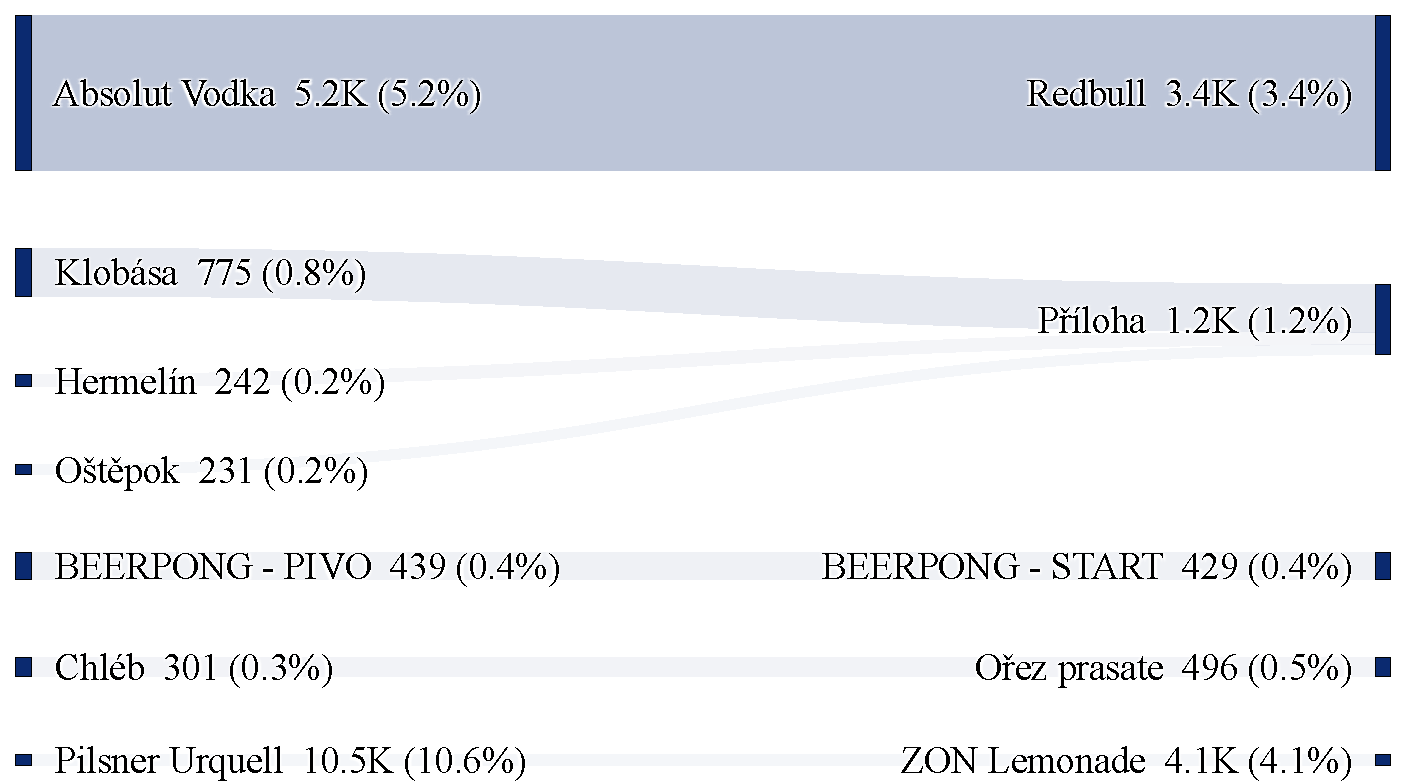
\includegraphics[width=\textwidth]{\ChartsDir/rq29-product-combos-without-returnable}
	\caption{\rqshorttext{customers-common-combinations} Most Common Product Combinations without Cups}
	\label{chart:common-combos-without-cups}
	\source
\end{chart}

This revealed the most popular product combination, without returnable cups included, was the \textbf{Absolut Vodka} and \textbf{Redbull} accounting to total of~\bfmtnump[2]{2.48}\%~of all transactions.

There was also a notable high combination of non-beverage products, such as \textbf{Klobása}, \textbf{Hermelín}, or \textbf{Oštěpok} in combination with \textbf{Příloha}, making it a seemingly popular food choice.

Interpretation of the results could have been done in many ways, for example, using a network graph to visualize the relationships between products.
This, as exciting as it sounded, was not in the end the most suitable way to present the results in a clear and concise manner.

\begin{keytakeaways}
	\begin{itemize}
		\item The most common product combination was \textbf{Absolut Vodka} and \textbf{Redbull} (\bfmtnump[2]{2.48}\%~of all transactions).
		\item The most common non-beverage combination was \textbf{Klobása} and \textbf{Příloha}.
		\item Returnable cups were, not surprisingly, a significant part of the most common combinations.
	\end{itemize}
\end{keytakeaways}

\subsection{Summary}
\label{subsec:analysis-customer-summary}

This section provided a thorough evaluation of festival attendees' habits, preferences, and segmentation.
It provided practical information about visitor interactions with the festival by analyzing trends in attendance, payment methods, purchase preferences, and event product combinations that contributed most to overall sales.

All previously defined questions were answered and presented in a simple and understandable way, providing hopefully valuable insights for the festival organizer.

%%% Section: Conclusion
%%% --------------------------------------------------------------


\section{Conclusion}
\label{sec:analysis-conclusion}

The analyses in this chapter provide a comprehensive look at the festival's behavior, including data-oriented insights on operational effectiveness, financial performance, and customer behavior.
By fully addressing every research question, the results provide an in-depth knowledge of the festival dynamics and offer practical suggestions for upcoming seasons.

Analysis of cash flow dynamics and income sources revealed important revenue-generating systems and their interactions.
Concurrent with this, performance indicators showed the system's ability to control transactional spikes and the ability to handle higher transaction
volumes\footnote{This was not surprising, as the system is designed and should be able to handle such transaction volumes in much larger quantities than at this festival}.

Analyzing the customer behavior revealed notable trends in attendance and buying preferences.

Furthermore, the analysis of beverage consumption highlighted how different beverage brands performed throughout the festival.
The distinctive trends in beverage preferences and their correlation with specific times of day highlight the possibility to adapt offers to satisfy customer needs.
It also showed the importance of having consistent product assortment configuration to be able to answer such questions.

This chapter laid the basis for the forthcoming dashboard development, which will try to demonstrate these findings in a more interactive way.

